\documentclass[12pt, a4paper]{report}

\usepackage[utf8]{inputenc}
\usepackage[french, arabic, main=english]{babel}
\usepackage{csquotes}
\usepackage[LAE, T1]{fontenc}
\usepackage{array}
\usepackage{amsmath, amssymb, amsfonts, amsthm}
\usepackage{bbm}
\usepackage[dvipsnames,svgnames]{xcolor}
\usepackage{fancyhdr}
\usepackage{graphicx}
\graphicspath{{assets/images}{assets/pdf}{assets/python}}
\usepackage[inline]{enumitem}
\usepackage{import}
\usepackage{colonequals}
\usepackage{hyperref}
\hypersetup{%
    colorlinks=true,
    linkcolor=DarkBlue,
    urlcolor=blue,
    citecolor=DarkGreen,
    pdfauthor={Mohammed Belgoumri},
    pdfkeywords={this is a kw}
}
\usepackage{cleveref}
\usepackage[top=2.5cm,bottom=2.5cm,right=2.5cm,left=2.5cm]{geometry}
\usepackage{appendix}
\usepackage{wrapfig}
\usepackage{cprotect}
\import{preambule}{tikz}

\newlength\figureheight
\newlength\figurewidth

\usepackage[backend=biber, style=apa]{biblatex}
\addbibresource{references.bib}

\usepackage{etoolbox}

\usepackage{caption}

\import{preambule}{codestyle}
%% Algorithm style
\usepackage[ruled,linesnumbered,nosemicolon]{algorithm2e}
\SetFuncArgSty{}
\definecolor{codegreen}{rgb}{0,0.6,0}
\newcommand{\mycomntsty}[1]{\texttt{\textcolor{codegreen}{#1}}}
\newlength{\commentWidth}
\setlength{\commentWidth}{7cm}
\SetCommentSty{mycomntsty}
\newcommand{\atcp}[1]{\tcp*[r]{\makebox[\commentWidth]{#1\hfill}}}
% no line break version of \atcp
\newcommand{\atcpl}[1]{\tcp*[f]{\makebox[\commentWidth]{#1\hfill}}}

\usepackage{arabtex}
\usepackage{utf8}
\setcode{utf8}

\usepackage{afterpage}
\usepackage{float}
\usepackage{subcaption}



\usepackage{stmaryrd}
\usepackage{bookmark}
\usepackage{booktabs}
\usepackage{stackengine}
\usepackage{adjustbox}
\usepackage{footnote}
\makesavenoteenv{tabular}
\makesavenoteenv{table}


\setlength{\parskip}{.4cm}
\import{preambule}{theorems}

% Fix the problem of \times (caused by babel or arabtex)
\renewcommand{\times}{\mathbin{\mathsf{x}}}


% Number sets
\newcommand{\complexes}{\mathbb{C}}
\newcommand{\reals}{\mathbb{R}}
\newcommand{\rationals}{\mathbb{Q}}
\newcommand{\integers}{\mathbb{Z}}
\newcommand{\naturals}{\mathbb{N}}
\newcommand{\field}{\mathbb{K}}


% Problems/ complexity classes
\newcommand{\TSP}{\textsf{TSP}}
\newcommand{\classP}{\textsf{P}}
\newcommand{\classNP}{\textsf{NP}}
\newcommand{\classNPO}{\textsf{NPO}}

% Math operators
\newcommand{\argmin}{\operatornamewithlimits{argmin}}
\newcommand{\argmax}{\operatornamewithlimits{argmax}}
\newcommand{\diff}[1]{\mathrm{d}#1}
\newcommand{\pdiff}[1]{\partial#1}


% default greeks
\let\uglyepsioln\epsilon
\let\epsilon\varepsilon

\let\roundphi\phi
\let\phi\varphi

% Landau notation
\newcommand{\bigO}[1]{\mathcal{O}\left(#1\right)}

% Probability
\newcommand{\prob}{\operatornamewithlimits{\mathbb{P}}}
\newcommand{\esp}{\operatornamewithlimits{\mathbb{E}}}

% Linear algebra
\newcommand{\tr}{\operatorname{tr}}


% ML
\newcommand{\softmax}{\operatorname{softmax}}
\newcommand{\relu}{\operatorname{ReLU}}

%citation style
\let\barecite\cite
\let\cite\parencite

\import{preambule}{abbreviations}
\usepackage[T1]{fontenc}
\usepackage[english]{babel} 
\usepackage{graphicx}
\usepackage{amsmath, amssymb}
\usepackage{hyperref}
\usepackage{geometry}
\usepackage{fancyhdr}
\usepackage{tocloft} 
\usepackage{listings}
\usepackage{float}
\usepackage{algorithm}
\usepackage{enumitem}
\usepackage{algpseudocode}
\usepackage{comment}
\usepackage{booktabs}
\usepackage{array} 
\usepackage{graphicx}  
\usepackage{array} 
\usepackage{pdflscape}
\usepackage{tabularx}
\usepackage{multirow}
\usepackage{amssymb}
\usepackage[ruled,vlined]{algorithm2e} 

% Add these packages for references
\usepackage[backend=biber,    % biber is the modern alternative to bibtex
            style=numeric,    % or 'authoryear', 'ieee', etc.
            sorting=none,     % or 'nyt' (name, year, title)
            natbib=true]{biblatex} % for \citet and \citep commands
\addbibresource{biblio.bib}  % your bibliography file

% !TEX root = main.tex
\begin{document}

\setcounter{tocdepth}{2}
\afterpage{
  \newgeometry{top=0.6in,bottom=0.6in,right=1in,left=1in}
  \begin{titlepage}
    \pagenumbering{gobble}
    \phantomsection\addcontentsline{toc}{chapter}{Cover page}

    \centering
    {\small République Algérienne Démocratique et Populaire}\\
    \RL{الجمهورية الجزائرية الديـموقراطية الشعبية}\\
    {\small Ministère de l'Enseignement Supérieur et de la Recherche Scientifique}\\
    \RL{وزارة التعليم العالي والبحث العلمي}\\
    \rule{\linewidth}{0.3mm} \\[0.4cm]

    \begin{minipage}{5cm}
      \begin{flushleft}
        
\includegraphics[width=4.9cm]{assets/images/esi_logo.png}
      \end{flushleft}
    \end{minipage}\hfill
    %%
    \begin{minipage}{10cm}
      \begin{flushright}
        \RL{المدرسة الوطنية للإعلام الآلي}\\
        (\RL{المعهد الوطني للتكوين في الإعلام الآلي سابقا})\\
        {\small École nationale Supérieure d'Informatique}\\[0.1cm]
        {\small ex. INI (Institut National de formation en Informatique)}\\[0.1cm]
      \end{flushright}
    \end{minipage}\hfill\\
    %%
    \vspace{20mm}
    %%
    {\large \bfseries Graduation Thesis}\\[0.5cm]
    {\large \bfseries For the Award of the State Engineer’s Degree in Computer Science }\\[0.5cm]
    {\large \bfseries specialization :  Software Engineering Systems and Computer Systems \\ }

    \vspace{10mm}

    % Title
    \rule{\linewidth}{0.3mm} \\[0.4cm]
    {
    \Large \bfseries
    Implementation of a communication system between drones and ground sensors for road traffic monitoring
    }
    %%
    \rule{\linewidth}{0.3mm} \\[1cm]

    \vspace{10mm}

    % Author and supervisor
    \noindent
    \begin{minipage}{0.6\textwidth}
      \vspace{-7mm}
      \begin{flushleft} \large
        \emph{Realized by :}\\
        \textsc{IFOURAH} Younes \\
        % \href{mailto:ky_ifourah@esi.dz}{\verb!ky\_ifourah@esi.dz!}
      \end{flushleft}
    \end{minipage}
    %%
    \begin{minipage}{0.35\textwidth}
      \begin{flushright} \large
        \begin{flushleft} \large
          \emph{Supervised by:} \\
          {
          M. \textsc{Balla} Amar\\[0.1cm]
          % \href{mailto:a_balla@esi.dz}{\verb!a\_balla@esi.dz!}\\
          M. \textsc{Boujit} Saadi\\[0.1cm]
          % \href{mailto:saadi.boudjit@univ-rouen.fr}{\verb!saadi.boudjit@univ-rouen.fr!}\\[0.1cm]
          Mme. \textsc{Bouzefrane} Samia\\[0.1cm]
          % \href{mailto:samia.bouzefrane@lecnam.net}{\verb!samia.bouzefrane@lecnam.net!}\\[0.1cm]
          Mme. \textsc{Boussaha} Ryma\\[0.1cm]
          % \href{mailto:r_boussaha@esi.dz}{\verb!r\_boussaha@esi.dz!}\\
          }
        \end{flushleft}
      \end{flushright}
    \end{minipage}\\[1cm]

    % \begin{minipage}{.7\linewidth}
    %   \begin{center}
    %     \begin{flushleft}
    %       \emph{Soutenu le 22 juin 2023, devant le jury composé de:}\\
    %       Dr. \textsc{Chebieb} AbdelKrim (ESI): Président\\
    %       Dr. \textsc{Hamani} Nacer (ESI): Rapporteur\\
    %       Dr. \textsc{Charabi} Leila (ESI): Examinateur\\
    %     \end{flushleft}
    %   \end{center}
    % \end{minipage}

    \vfill

    {\large 2024 / 2025}
  \end{titlepage}
  \restoregeometry
}
\renewcommand{\headrulewidth}{0pt}
\fancypagestyle{plain}{\fancyhf{}\cfoot{\thepage}}
\vfill{}
\begin{center}
    {
        \Large\bfseries
        Dédicace  % Changed from \RL{dedication} to normal French
    }
\end{center}

À mes parents,
Merci pour votre amour inconditionnel, votre patience et les valeurs profondes que vous m’avez transmises. Vous m’avez appris à croire en moi, à faire preuve de rigueur, à persévérer même dans les moments les plus difficiles. Votre présence à mes côtés a été le socle sur lequel j’ai pu bâtir ce parcours. Ce travail est en grande partie le fruit de votre dévouement.

À mon grand-père, paix à son âme,
Son souvenir continue d’illuminer mon chemin. Sa sagesse, sa bonté et ses paroles résonnent encore en moi, comme une source de réconfort et de force dans les épreuves. Ce travail est aussi un hommage à sa mémoire.

À ma famille,
Merci pour votre tendresse, vos encouragements et vos prières silencieuses qui m’ont toujours accompagné. Votre soutien discret mais constant a été essentiel à chaque étape de cette aventure.

À mes amis,
Pour les sourires partagés, les échanges sincères et les instants de légèreté qui ont su alléger la charge des moments plus rudes. Votre présence a donné à ce parcours une chaleur irremplaçable.

À mes enseignants,
De l’école aux études supérieures, merci d’avoir éveillé en moi la curiosité, le goût de l’effort et le désir d’apprendre toujours davantage. Votre confiance m’a souvent donné la force de dépasser mes limites.

\vfill{}
\pagebreak
\vfill{}
\begin{center}
    {
        \Large\bfseries
        Remerciements  % Removed \RL
    }
\end{center}

Je tiens à remercier chaleureusement ma directrice de projet pour son accompagnement attentif, la pertinence de ses retours et la clarté de ses conseils. Son encadrement m’a permis d’avancer avec méthode et de donner plus de profondeur à ce travail.

Je suis également très reconnaissant envers ma co-encadrante pour son soutien constant, ses conseils avisés et ses encouragements tout au long du projet. Sa disponibilité et sa bienveillance ont été d’une aide précieuse.

Mes remerciements vont aussi à l’équipe administrative et technique, dont le soutien logistique m’a permis de travailler dans de très bonnes conditions, avec les ressources nécessaires à la réalisation de mes expérimentations.

Ces années d’études resteront pour moi une période marquante, rythmée par des rencontres humaines et professionnelles enrichissantes. Je garderai en mémoire les échanges avec mes camarades, les enseignements reçus, ainsi que toutes les personnes croisées au quotidien.

Enfin, je remercie du fond du cœur ma famille et mes amis, pour leur présence constante, leur soutien moral et leur compréhension tout au long de ce parcours.

À toutes celles et ceux qui, de près ou de loin, ont contribué à la concrétisation de ce travail : un grand merci.

\vfill{}
\pagebreak
\vfill{}
\begin{center}
    {
        \Large\bfseries
        Resume  % Removed \RL
    }
\end{center}

Ce mémoire de fin d'études explore la mise en œuvre d'un système de communication novateur entre drones et capteurs au sol pour la surveillance du trafic routier. Face aux limitations des systèmes de surveillance traditionnels, l'intégration des Véhicules Aériens Sans Pilote (UAVs) offre des solutions prometteuses pour une gestion du trafic plus efficace.

Le document débute par une analyse approfondie des architectures des UAVs (multirotors, voilures fixes, hybrides) et de leurs caractéristiques opérationnelles (poids, endurance, portée, altitude). Il explore ensuite les protocoles de communication spécifiques aux UAVs tels que MAVLink, UranusLink et UAVCAN, en mettant en avant leurs avantages et leurs limitations, notamment en termes de sécurité et d'efficacité des ressources. Les différentes architectures de communication en essaim (centralisée, décentralisée à groupe unique, multi-groupes et multi-couches) ainsi que les protocoles de routage associés (basés sur la topologie, la position ou l'intelligence en essaim) sont également détaillés, soulignant leur impact sur la scalabilité et la robustesse.

Une partie substantielle du travail est consacrée à l'intégration de l'Intelligence Artificielle (IA) et des techniques d'apprentissage automatique (ML) pour optimiser les performances des UAVs. Cela inclut l'amélioration de la planification de trajectoire, de la gestion des missions, de la perception et de l'extraction de caractéristiques à travers des méthodes d'apprentissage supervisé, non supervisé et par renforcement (comme les Deep Q-Networks et Deep Deterministic Policy Gradient). Le mémoire aborde également les défis de sécurité cruciaux dans les réseaux d'UAVs, en identifiant les menaces (écoute clandestine, brouillage, attaques de l'homme du milieu, attaques par rejeu, portes dérobées, déni de service) et en présentant les solutions existantes pour garantir l'intégrité et la confidentialité des communications.

En conclusion, ce travail souligne que malgré les avancées significatives, des défis subsistent concernant l'endurance opérationnelle, la stabilité des communications et les cadres réglementaires. L'innovation continue dans les systèmes énergétiques, les protocoles réseau et le développement de politiques sera cruciale pour l'adoption généralisée des UAVs dans les infrastructures de transport intelligentes du futur.

\vfill{}
\pagebreak

\begin{abstract}
    \thispagestyle{plain}
    \pagenumbering{roman}
    \setcounter{page}{2}
    \phantomsection\addcontentsline{toc}{chapter}{\abstractname}


    Aphasia is a language disorder caused by brain damage (most commonly a stroke).
    Broca's aphasia is a form of aphasia that impairs language production.
    It is caused by an injury to Broca's Area, an area of the frontal lobe of the brain; responsible for language decoding.
    A person suffering from Broca's aphasia may find it difficult to articulate words and sentences.
    However, they generally can understand what is said to them.
    This form of aphasia is associated with a lower quality of life and a higher risk of depression and suicide.

    Speech therapy is the most commonly prescribed remedy to people with Broca's aphasia.
    Despite its effectiveness, it remains an expensive, time-consuming, and effort-heavy process.
    This makes it inaccessible to a significant number of people with aphasia.

    The use of natural language processing-based techniques to improve these people's quality of life
    is an emerging research avenue that has enjoyed the attention of many researchers in recent years.

    In this graduation project,
    we are interested in the use of machine translation and automatic speech recognition
    to partially automate the rehabilitation of people with aphasia.

    To this end, we conduct a bibliographic study in which introduce aphasia, its causes, consequences,
    the problems of classical treatment methods, and a literature review the existing works
    pertaining to machine translation and automatic speech recognition.

    We then design a system that corrects french aphasic speech
    by combining a translation model with a speech recognition model, the former of which we implement.
    We finish by presenting the results of our work:
    a corpus for automatic speech recognition,
    and a translation model with a {bleu} score of \(79.61\%\).
    %%
    \\ [2cm]
    %%
    \rule{\linewidth}{1pt}

    \textbf{Keywords --- } Broca aphasia, Machine learning, Natural language processing, Machine translation, Automatic speech recognition, Transformer.\\
    \rule{\linewidth}{1pt}
\end{abstract}


\begin{otherlanguage}{french}
    \begin{abstract}
        \thispagestyle{plain}
        \pagenumbering{roman}
        \setcounter{page}{1}
        \phantomsection\addcontentsline{toc}{chapter}{\abstractname}

        Ceci est un résumé en français.

        %%
        \ \\[2cm]
        %%
        \rule{\linewidth}{1pt}

        \textbf{Mots clés --- } Aphasie de Broca, Transformeur.\\
        \rule{\linewidth}{1pt}
    \end{abstract}

\end{otherlanguage}



% \renewcommand{\abstractname}{\RL{مـلـخـص}}
% \afterpage{
%     \newgeometry{top=-2cm}
%     \begin{abstract}
%         \thispagestyle{plain}
%         \pagenumbering{roman}
%         \setcounter{page}{3}
%         \phantomsection\addcontentsline{toc}{chapter}{\textRL{مـلـخـص}}
%         \begin{RLtext}
%             الـحـبـسـة إضـطـرابٌ لـغـوي نـاتـج عن تـلـف فـي الـدمـاغ، غـالـبـا نـتـيـجـة سـكـتـة دمـاغـيـة.
%             حـبـسـة بـروكـا حـبـسـة تـنـتـج عـن إصـابـة فـي مـنـطـقـة بـروكـا،
%             وهـي مـنـطـقـة فـي الـفـص الجـبـهي الأيـسـر للـدمـاغ تـعـنـى بـإنـتـاج الكـلام.
%             قـد يـجـد الـمـصـاب بـحـبـسـة بـروكـا صـعـوبـة فـي تـكـويـن الـجـمـل والـكـلـمـات،
%             إلا أنـه عـادة يـفـهـم مـا يـقـال.
%             تـرتـبـط هـذه الحـبـسـة بـتـدنـي مـسـوى الـعيـش وارتـفتاع  خـطر الاكـتـئـاب والانـتـحـار.

%             عـلاج الـنـطق هـو أكـثـر الـعـلاجـات وصـفـا للمـصـابـيـن بـحـبـسـة بـروكـا.
%             رغـم نـجـاعـتـه، فـهو يـظـل مـكـلـفـا للـوقـت والـمـال والـجـهـد،
%             مـا يـحـول دون تـوفـره لعـدد كـبـيـر مـمـن يـحـتـاجـونـه.

%             تـوظـيـف تـقـنـيـات مـعـالـجـة اللـغـة الـطـبـيـعـيـة لـتـحـسـيـن حـيـاة الـمـصـابـيـن بـحـبـسـة بـروكـا
%             مـجـال بـحـث حـظي بـاهـتـمـام الـعـديـد مـن الـبـاحـثـيـن فـي الأعـوام الأخـيـرة.

%             فـي مـشـروع الـتـخـرج هـذا، نـهـتـم بـاسـتـعـمـال الـتـرجـمـة الآلـية والـتـعرف الآلـي عـلى الكـلام
%             لتـأديـة جـزء مـن عـلاج الـنـطق لـحـبـسـة بـروكـا أوتـومـاتـيـكـيـا.
%             مـن أجـل ذلك، نـعـرض دراسـة بـيـبـلـيـوغـرافـيـة
%             نـعـرف فـيـهـا بـحـبـسـة بـروكـا أسـبـابـا ونـتـائـج،
%             ثـم نـتـطرق لـعـيـوب الـعـلاجـات الـمـعـتـادة.
%             وللأعـمـال الـتـي سـبـق إنـجـازهـا فـي مـجـالـي الـتـرجـمـة الآلـية والـتـعرف الآلـي عـلى الكـلام.

%             نـأتـي بـعـدهـا إلـى تـصـمـيـم نـظام لـتـصـحـيـح الـكـلام الـمـحـتـبـس بـاللـغـة الـفـرنـسـيـة
%             يـجـمـع بـيـن نـمـوذجـيـن، أحـدهـمـا للـتـعرف الآلـي عـلى الكـلام والآخـر للـتـرجـمـة الآلـيـة
%             ونـعـرض إنـجـاز هـذا الأخـيـر.
%             نـخـتـم أخـيـرا بـعـرض نـتـائـج هـذا الـعـمـل مـتـمـثـلـة فـي مـجـمـوعـة بـيـانـات للـتـعرف الآلـي عـلى الكـلام
%             ونـمـوذج للـتـرجـمـة الآلـيـة تـقـيـيـمـه بـمـقـيـاس \LR{{bleu}} يـسـاوي \(79.61\%\).
%         \end{RLtext}
%         \hspace*{0mm}\rule{\linewidth}{1pt}
%         \begin{RLtext}
%             \textbf{الـكـلـمـات الـمـفـتـاحـيـة ـــ } حـبـسـة بـروكـا،
%             تـعـلم الآلـة،
%             مـعـالـجـة اللـغـة الـطـبـيـعـيـة،
%             تـرجـمـة آلـيـة،
%             تـعرف آلـي عـلى الكـلام،
%             شـبـكـة عـصـبـيـة غـيـر تـرتـيـبـيـة.\\
%         \end{RLtext}
%         \rule{\linewidth}{1pt}
%     \end{abstract}
%     \restoregeometry
% }
\afterpage{
    \newgeometry{bottom=3cm}
    \tableofcontents
    \addcontentsline{toc}{chapter}{Contents}
    \listoffigures
    \addcontentsline{toc}{chapter}{List of figures}
    
    % \lstlistoflistings
    % \addcontentsline{toc}{chapter}{List of \lstlistlistingname}
    % \listofalgorithms
    % \addcontentsline{toc}{chapter}{List of Algorithms}
}

\restoregeometry
\pagenumbering{arabic}
% \setcounter{page}{1}
\chapter*{General introduction}
\addcontentsline{toc}{chapter}{General introduction}
\label{chap.intro}

The introduction goes here.

\chapter{UAV Topologies, standards and Communication Protocols}
\section{Introduction}



In recent years, Unmanned Aerial Vehicles (UAVs) have evolved from specialized military tools into versatile platforms used in a wide range of civilian and commercial applications. This rapid development has resulted in a variety of UAV types, each designed for specific missions and operational needs. To better understand the technological landscape of UAVs, it is essential to examine their structural configurations, classification methods, and communication systems. This chapter presents an overview of UAV architectures from both design and performance perspectives. It also explores the key standards and communication protocols that enable their operation. The objective is to provide a clear picture of the current technological state of UAVs and their potential for integration into advanced systems.


%\subsection{History of Drones} 
\section{UAV Classification}


%%%%%%%%%%%%%%%%%%%%%%%%%%%%%%%%%%%%%%%%%%%%%%%%%%%%%%%%%%%%%%%%%%%%%%
%%%%%%%%%%%%%%%%%%%%%%%%%%%%%%%%%%%%%%%%%%%%%%%%%%%%%%%%%%%%%%%%%%%%%%
%%%%%%%%%%%%%%%%%%%%%%%%%%%%%%%%%%%%%%%%%%%%%%%%%%%%%%%%%%%%%%%%%%%%%%


Unmanned Aerial Vehicles (UAVs) have recently exhibited significant diversity in terms of design, functionality, and mission-specific adaptability. As their use expands across both civilian and military sectors, a robust classification framework becomes essential for understanding and optimizing their deployment. UAVs can be broadly categorized based on two major axes: \textbf{performance metrics} and \textbf{design architectures}.

\vspace{0.5cm}

\textit{Performance-based classification} involves measurable operational characteristics such as \textit{weight}, \textit{endurance}, \textit{range}, \textit{speed}, \textit{altitude}, \textit{wing loading}, and \textit{engine type}. These parameters are critical in determining how well a UAV meets specific mission requirements, such as long-range reconnaissance or high-speed target tracking.

\vspace{0.5cm}

In contrast, \textit{design-based classification} provides a structural perspective, focusing on aspects such as the \textit{aerodynamic configuration}, the \textit{number and arrangement of rotors or motors}, and the overall \textit{geometrical form}. This classification helps in understanding the UAV's flight behavior, stability, payload capacity, and maneuverability in various environments.


\begin{figure}[H]  % 'h' means place the figure "here" if possible
    \centering
    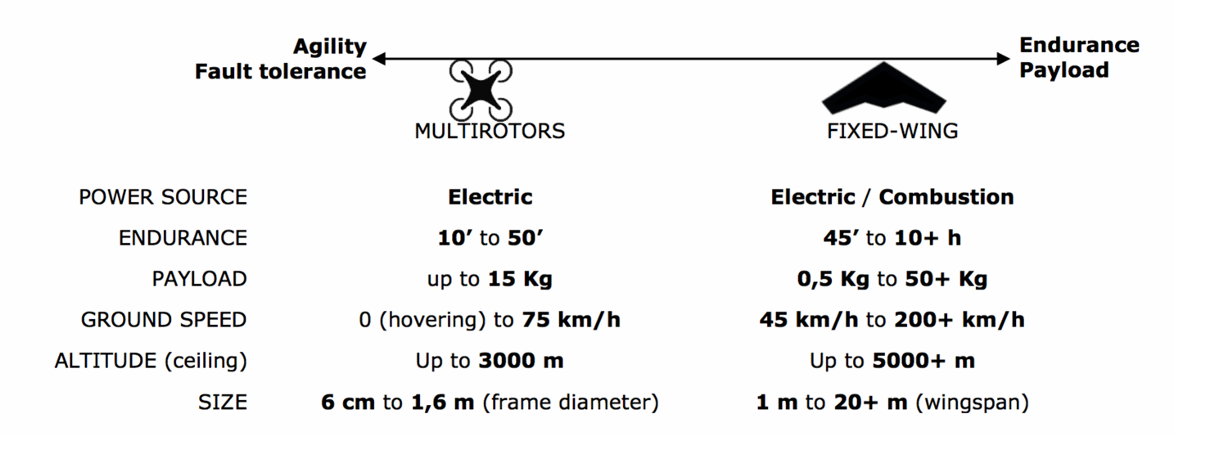
\includegraphics[width=0.7\textwidth]{Figures/Chapter1/Section1/1.png} % Adjust width as needed
    \caption{ Capabilities of fixed-wing/multi-rotors (adapted from: \cite{khan2024smarttraffic})}
    \label{fig:method3_architecture} % Reference label
\end{figure}


%%%%%%%%%%%%%%%%%%%%%%%%%%%%%%%%%%%%%%%%%%%%%%%%%%%%%%%%%%%%%%%%%%%%%%


\subsection{Design-Based Classification}

Design architecture plays a pivotal role in UAV functionality. UAVs can be structurally categorized into the following primary types. Figure~\ref{fig:uav_design_types} provides an overview of the primary UAV types based on design architecture.

\begin{figure}[H]  % 'h' means place the figure "here" if possible
    \centering
    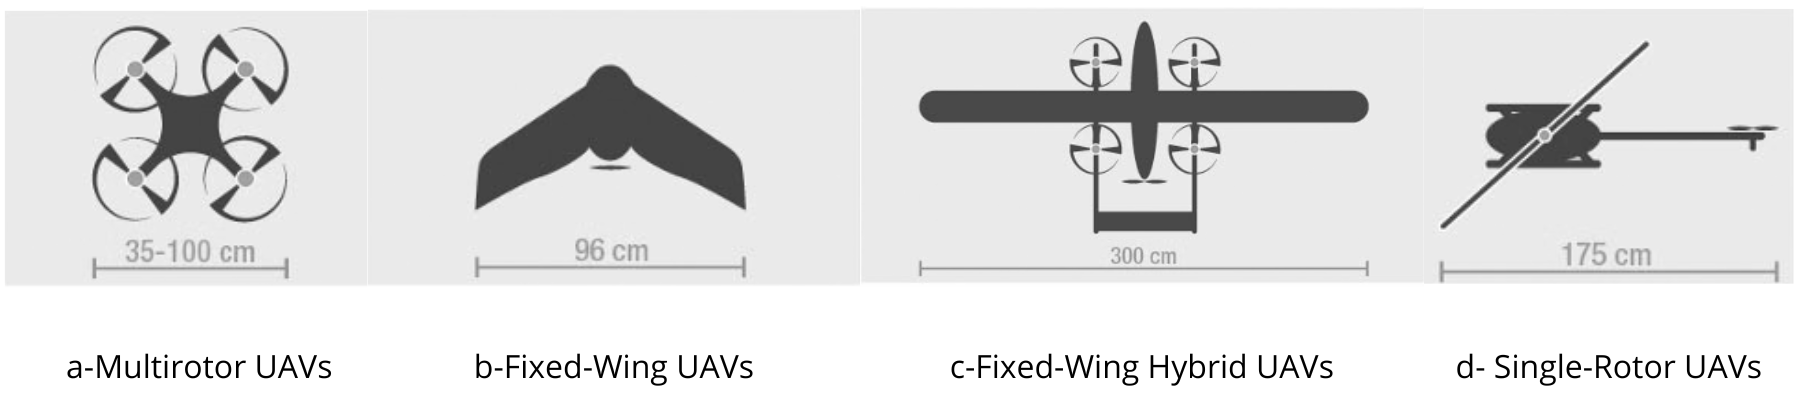
\includegraphics[width=0.7\textwidth]{Figures/Chapter1/Section1/11.png} % Adjust width as needed
    \caption{ Illustration of UAV Types Classified by Design )}
    \label{fig:uav_design_types}
\end{figure}


\begin{itemize}
    \item \textbf{Multirotor UAVs:} This category includes the most common drones used in commercial and consumer applications, featuring multiple rotors that allow for vertical lift, precise control, and stable hovering. Multirotor UAVs are typically employed in aerial photography, inspection, and surveillance tasks. The main types of multirotors are as follows:

    \begin{figure}[H]  % 'h' means place the figure "here" if possible
        \centering
        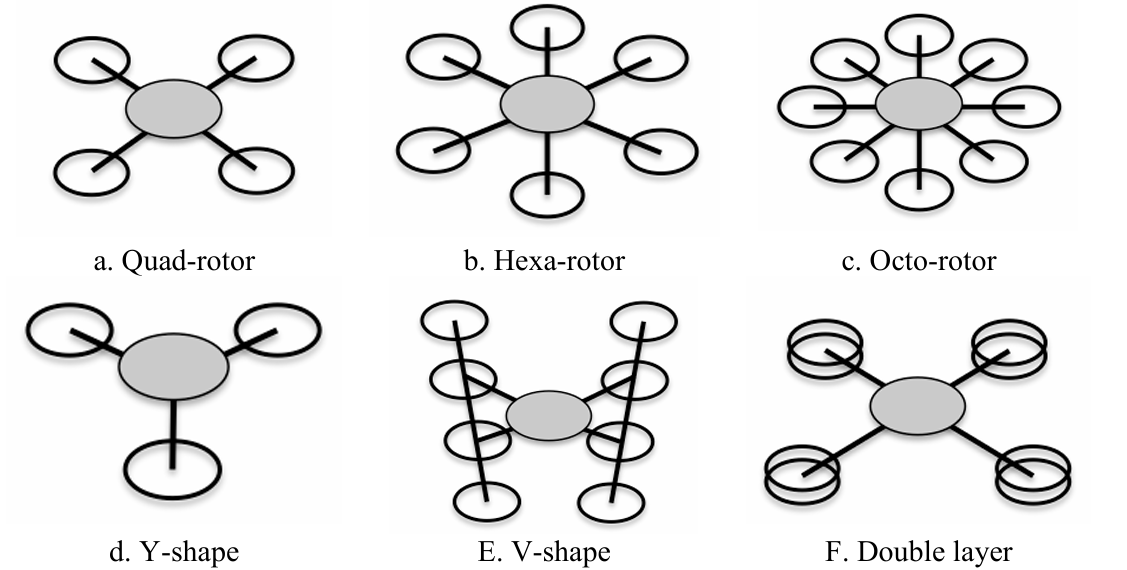
\includegraphics[width=0.7\textwidth]{Figures/Chapter1/Section1/2.png} % Adjust width as needed
        \caption{  Multi-rotors Layout  (adapted from: \cite{chen2016state})}
        \label{fig:method3_architecture} % Reference label
    \end{figure}
    
\begin{itemize}
    \item \textbf{Quad-rotor (4 Rotors):} Most common and cost-effective, offering stability for light-to-medium payloads. Limited redundancy single motor failure can destabilize flight. \cite{idk}
    
    \item \textbf{Hexa-rotor (6 Rotors):} Improved redundancy and payload capacity over quadcopters. Can tolerate one rotor failure but consumes more power. \cite{idk}
    
    \item \textbf{Octo-rotor (8 Rotors):} Highest redundancy and payload capacity, suited for critical missions. Sacrifices flight time due to high power demand. \cite{idk}
    
    \item \textbf{Y-shape Layout:} Three-rotor design for space efficiency. Lower redundancy and stability compared to quad/hexa configurations. \cite{idk}
    
    \item \textbf{V-shape Layout:} Aerodynamic efficiency for longer flight times. Compromises redundancy and stability. \cite{idk}
    
    \item \textbf{Double Layer Configuration:} Stacked rotors enhance lift in compact designs. Increases complexity and power usage. \cite{idk}
\end{itemize}
    
    \item \textbf{Fixed-Wing UAVs:} Fixed-wing UAVs generate lift via rigid wings, offering high efficiency for long-distance missions like mapping and surveying \cite{ucgun2021uavcharging}. They excel in speed and endurance but require runways for takeoff/landing, lacking VTOL capabilities. Compared to multirotors, they cover larger areas faster, making them ideal for large-scale data collection. Typical applications include military, agricultural, and scientific operations requiring extended flight times and higher payloads.

    % \begin{figure}[H]  % 'h' means place the figure "here" if possible
    %     \centering
    %     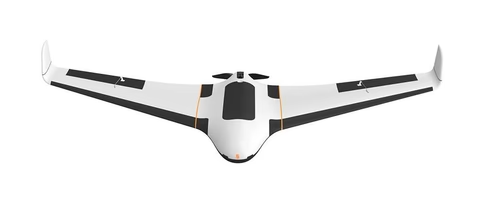
\includegraphics[width=0.7\textwidth]{Figures/Chapter1/Section1/3.png} 
    %     \caption{  Fixed-Wing UAVs (adapted from: site web uavsystemsinternational.com)}
    %     \label{fig:method3_architecture} % Reference label
    % \end{figure}

    \item \textbf{Fixed-Wing Hybrid UAVs:} Fixed-wing hybrid UAVs merge fixed-wing efficiency with rotary-wing VTOL capabilities, enabling flexible operation without runways. Their dual design allows long-range flight and quick deployment in confined spaces, ideal for search-and-rescue or surveillance. However, they are more complex and heavier than pure fixed-wing or multirotor UAVs.

    \item \textbf{Single-Rotor UAVs:} Single-rotor UAVs, like helicopters, use a main rotor for lift and a tail rotor for stability. They are more energy-efficient than multirotors, especially for heavy payloads, but have higher complexity and maintenance costs. Their advantages include longer flight times, better wind resistance, and suitability for cargo transport, surveying, and industrial inspections.
    
\end{itemize}

This classification provides a clear understanding of the different UAV types and their specific use cases based on design. Whether the goal is to achieve high endurance, heavy payload capabilities, or versatility in flight control, selecting the appropriate UAV design is essential for optimizing performance in various applications.



%%%%%%%%%%%%%%%%%%%%%%%%%%%%%%%%%%%%%%%%%%%%%%%%%%%%%%%%%%%%%%%%%%%%%%


\subsection{Performance-Based Classification}

Complementing the structural design perspective, UAVs can also be evaluated based on core operational parameters:

\begin{enumerate}
    \item \textbf{Weight:} Influences lift requirements, battery life, and legal classifications.

    UAVs span a wide spectrum of weights from micro UAVs under 5 kg to large strategic drones like the \textit{Global Hawk}, which exceeds 11 tonnes. Based on their take-off weight, UAVs can be classified into five categories:

    % \begin{itemize}
    %     \item \textbf{Micro UAVs (MAV):} Under 5 kg. Examples include the Dragon Eye, FPASS, Pointer, and SilentEyes.
    %     \item \textbf{Lightweight UAVs:} Between 5 kg and 50 kg.
    %     \item \textbf{Medium UAVs:} From 50 kg to 200 kg, such as the Raven up to the Phoenix.
    %     \item \textbf{Heavy UAVs:} Between 200 kg and 2000 kg, covering platforms like the Outrider to the Fire Scout.
    %     \item \textbf{Super Heavy UAVs:} Over 2 tonnes. This includes high-performance UAVs like the X-45, Predator B, Darkstar, and Global Hawk.
    % \end{itemize}

    \begin{table}[h]
        \centering
        \label{tab:uav_weights}
        \begin{tabular}{|l|l|l|}
        \hline
        \textbf{Category} & \textbf{Weight Range} & \textbf{Examples} \\ \hline
        Micro UAVs (MAV) & <5 kg & Dragon Eye, FPASS, Pointer \\ \hline
        Lightweight UAVs & 5-50 kg & - \\ \hline
        Medium UAVs & 50-200 kg & Raven, Phoenix \\ \hline
        Heavy UAVs & 200-2000 kg & Outrider, Fire Scout \\ \hline
        Super Heavy UAVs & >2000 kg & Global Hawk, X-45, Predator B \\ \hline
        \end{tabular}
        \caption{UAV Weight Classifications and Implications}
    \end{table}

    These categories influence design decisions across multiple domains: \textit{heavier UAVs require greater lift and thrust}, often leading to increased wingspan and a shift in engine technology (e.g., electric motors for light UAVs, turbojets or turbofans for super heavy ones).

    \item \textbf{Endurance and Range:} Critical for determining the mission duration and operational area.

    Endurance and range are often interdependent and essential for mission planning, especially in military and surveillance operations. UAVs can be grouped based on their time aloft:


    \begin{table}[h]
        \centering
        \label{tab:uav_endurance}
        \begin{tabular}{|l|l|l|}
        \hline
        \textbf{Category} & \textbf{Duration} & \textbf{Examples} \\ \hline
        Short Endurance & <5 hours & "Over-the-hill" reconnaissance UAVs \\ \hline
        Medium Endurance & 5-24 hours & Shadow 600, Predator \\ \hline
        Long Endurance & $\geq$24 hours & Global Hawk (1500-22000 km range) \\ \hline
        \end{tabular}
        \caption{UAV Endurance Classifications}
    \end{table}


    
    % \begin{itemize}
    %     \item \textbf{Short Endurance:} Less than 5 hours. Typically used for brief tactical missions like "over-the-hill" reconnaissance.
    %     \item \textbf{Medium Endurance:} Between 5 and 24 hours. Includes UAVs like the Shadow 600 and Predator this is the most common endurance class.
    %     \item \textbf{Long Endurance:} 24 hours or more. These UAVs are capable of extended surveillance with ranges starting at 1500 km and reaching up to 22000 km, as demonstrated by the Global Hawk.
    % \end{itemize}

    These parameters directly impact logistical planning, including launch site placement and refueling intervals.

    \item \textbf{Maximum Altitude:} Defines the UAV’s vertical operational limit, often constrained by regulatory frameworks.

    Maximum flight ceiling is critical in both civilian airspace integration and military stealth operations. UAVs are divided into:


    \begin{table}[h]
        \centering
        \label{tab:uav_altitude}
        \begin{tabular}{|l|l|l|}
        \hline
        \textbf{Category} & \textbf{Altitude Range} & \textbf{Examples} \\ \hline
        Low Altitude & Below 1,000 m & FPASS, Pointer, Dragon Eye \\ \hline
        Medium Altitude & 1,000-10,000 m & (Most common UAVs) \\ \hline
        High Altitude & Above 10,000 m & X-45, Predator B, Global Hawk \\ \hline
        \end{tabular}
        \caption{UAV Altitude Classifications}
    \end{table}



    % \begin{itemize}
    %     \item \textbf{Low Altitude:} Below 1000 meters. Examples include micro UAVs like the FPASS, Pointer, and Dragon Eye. These are mostly experimental or limited in use.
    %     \item \textbf{Medium Altitude:} Between 1000 m and 10000 m. The majority of UAVs fall into this category.
    %     \item \textbf{High Altitude:} Above 10000 m. This includes advanced UAVs like the X-45, Predator B, Darkstar, and Global Hawk. Operating at this altitude raises airspace integration concerns, necessitating advanced collision avoidance systems.
    % \end{itemize}

    \item \textbf{Wing Loading:} Affects aerodynamic performance, especially in varying weather conditions.

    Wing loading is defined as the UAV's weight divided by its wing area. It influences flight stability, speed, and maneuverability:

    \begin{table}[h]
        \centering
        \label{tab:uav_propulsion}
        \begin{tabular}{|l|l|l|}
        \hline
        \textbf{Propulsion} & \textbf{Application} & \textbf{Advantages} \\ \hline
        Electric & <50 kg UAVs & Zero emissions, simple control \\ \hline
        Piston & 50-2000 kg UAVs & Fuel flexibility, proven reliability \\ \hline
        Turbofan/Turbojet & >2000 kg UAVs & Supersonic capability, high altitude \\ \hline
        Turboprop & 500-5000 kg UAVs & Efficient cruise performance \\ \hline
        \end{tabular}
        \caption{UAV Propulsion Systems by Performance Characteristics}
    \end{table}

    High wing loading tends to enhance performance in strong winds but may reduce lift efficiency at lower speeds.

    \item \textbf{Engine Type:} Determines propulsion efficiency, noise levels, and maintenance needs.

    UAV engines vary widely based on mission needs. Common engine types include:

    \begin{table}[h]
        \centering
        \label{tab:uav_propulsion}
        \begin{tabular}{|l|l|l|}
        \hline
        \textbf{Propulsion} & \textbf{Application} & \textbf{Advantages} \\ \hline
        Electric & <50 kg UAVs & Zero emissions, simple control \\ \hline
        Piston & 50-2000 kg UAVs & Fuel flexibility, proven reliability \\ \hline
        Turbofan/Turbojet & >2000 kg UAVs & Supersonic capability, high altitude \\ \hline
        Turboprop & 500-5000 kg UAVs & Efficient cruise performance \\ \hline
        \end{tabular}
        \caption{UAV Propulsion Systems by Performance Characteristics}
    \end{table}

    \textit{Engine type is often interrelated with weight, endurance, and range.} Proper selection can significantly improve mission performance and energy efficiency.

    % \item \textbf{Power/Thrust Loading:} Indicates the UAV's ability to accelerate and maintain flight under load.

    This ratio reflects how efficiently a UAV can generate thrust relative to its weight. High thrust loading implies better climb rates and maneuverability, crucial in tactical and high-speed operations. Conversely, low thrust loading may indicate endurance-focused platforms optimized for loitering rather than agility.
\end{enumerate}

UAV performance depends on weight, endurance, altitude, wing loading, and propulsion. These factors determine mission capabilities, from short-range electric drones to long-endurance turbine-powered systems. Each design choice involves trade-offs between speed, stability, and efficiency.

%%%%%%%%%%%%%%%%%%%%%%%%%%%%%%%%%%%%%%%%%%%%%%%%%%%%%%%%%%%%%%%%%%%%%%


\subsection{Discussion}

The two classification approaches design-based  and performance-based offer complementary perspectives for UAV analysis. Design determines fundamental capabilities, while performance metrics define operational limits. Hybrid designs bridge gaps but introduce trade-offs in complexity.

\vspace{0.5cm}

Design dictates how a UAV flies, while performance defines how well it executes missions. Together, they form a framework for selecting UAVs tailored to specific applications, balancing structural advantages with operational requirements.

\subsubsection{}


%%%%%%%%%%%%%%%%%%%%%%%%%%%%%%%%%%%%%%%%%%%%%%%%%%%%%%%%%%%%%%%%%%%%%%
%%%%%%%%%%%%%%%%%%%%%%%%%%%%%%%%%%%%%%%%%%%%%%%%%%%%%%%%%%%%%%%%%%%%%%
%%%%%%%%%%%%%%%%%%%%%%%%%%%%%%%%%%%%%%%%%%%%%%%%%%%%%%%%%%%%%%%%%%%%%%


\section{UAV Characteristics}

Unmanned Aerial Vehicles (UAVs) come in a variety of configurations and are designed for different purposes, including surveillance, reconnaissance, and commercial applications. The performance of a UAV depends on several characteristics such as speed, flight time, payload capacity, range, and altitude. These parameters play a crucial role in determining the UAV's efficiency, mission capability, and operational limits. This section discusses the key characteristics of UAVs, providing an overview of the factors that influence their behavior and utility.


%%%%%%%%%%%%%%%%%%%%%%%%%%%%%%%%%%%%%%%%%%%%%%%%%%%%%%%%%%%%%%%%%%%%%%


\subsection{Speed and Flight Time}

The speed and flight time of UAVs are critical factors that determine their performance during operations. Smaller UAVs typically have a lower maximum speed, often less than 15 m/s, while larger UAVs can reach speeds up to 100 m/s. Speed plays an essential role in optimizing the energy consumption of UAVs, especially when following a specific trajectory designed for spectral or energy efficiency. As discussed in \cite{ref52}, there is a trade-off between a UAV's turning agility and its speed, which should be considered when planning flight paths.

\vspace{0.5cm}

Flight time, on the other hand, refers to the maximum duration a UAV can remain airborne before its battery is drained. Factors such as the UAV's size, weight, and external weather conditions significantly affect battery life. Larger UAVs generally have the capability to fly for several hours, while smaller UAVs may only remain in the air for 20–30 minutes. The autopilot system and GPS functionality can also influence flight time. With the growing demand for UAVs in various industries, improving their flight time is essential. Thus, ongoing research focuses on overcoming the limitations of battery life, which is crucial for the wide-scale deployment of UAVs in both military and commercial sectors.


%%%%%%%%%%%%%%%%%%%%%%%%%%%%%%%%%%%%%%%%%%%%%%%%%%%%%%%%%%%%%%%%%%%%%%


\subsection{Payload}

The payload capacity of a UAV refers to its ability to carry various loads, such as sensors, cameras, and other equipment. Payloads typically range from a few grams to hundreds of kilograms, depending on the UAV's size and design. The payload directly impacts the UAV's performance, as carrying heavier loads generally reduces its flight time, increases battery consumption, and requires a larger frame. For instance, UAVs often carry sensors and video cameras for surveillance, reconnaissance, or commercial purposes.

\vspace{0.5cm}

Additionally, UAVs can transport cellular user equipment (UE), such as mobile phones or tablets, with a weight of less than 1 kg. It is important to note that while heavier payloads can reduce flight time, UAVs with larger surface areas and additional motors can store more power, potentially extending flight duration. Therefore, the design of the UAV and the quality of the payload play a crucial role in determining its operational efficiency and endurance.


%%%%%%%%%%%%%%%%%%%%%%%%%%%%%%%%%%%%%%%%%%%%%%%%%%%%%%%%%%%%%%%%%%%%%%


\subsection{Range and Altitude}

The range and altitude of a UAV are key performance indicators that affect its operational capabilities. Range refers to the distance over which a UAV can be controlled remotely, varying from just a few meters for small drones to several hundred kilometers for larger UAVs. Altitude, on the other hand, defines the maximum height a UAV can achieve during flight. UAVs are typically categorized based on their operating altitude into two primary categories: low altitude platforms (LAPs) and high altitude platforms (HAPs).

\vspace{0.5cm}

\textbf{Low Altitude Platforms (LAPs):} LAPs are designed to support cellular communication systems and are typically deployed for quick and cost-effective operations. They offer line-of-sight (LoS) paths, which significantly enhance communication performance \cite{ref54}. These platforms are ideal for short-range missions and are often used in urban environments or areas with limited infrastructure.

\vspace{0.5cm}

\textbf{High Altitude Platforms (HAPs):} In contrast, HAPs, such as balloons, provide broader coverage and are used for more extensive communication or Internet connectivity services. The deployment of HAPs is more complex and generally requires advanced technology and infrastructure. While HAPs are capable of covering vast areas, they are typically utilized in more specialized applications, including large-scale communications or satellite-like coverage.

\vspace{0.5cm}

% Table \ref{tab:uav_categories} and Figure \ref{fig:uav_projects} further illustrate the differences between UAV types based on their altitude and operational range.


%%%%%%%%%%%%%%%%%%%%%%%%%%%%%%%%%%%%%%%%%%%%%%%%%%%%%%%%%%%%%%%%%%%%%%


\subsection{UAV Principal Movements}

UAVs rely on specific movements to navigate and perform tasks effectively. These movements are influenced by the design of the UAV and its control systems. The principal movements of UAVs can be broadly categorized as follows:

\vspace{0.5cm}

\textbf{1. Pitch:} The pitch movement refers to the rotation of the UAV around its lateral axis, which runs from one side of the aircraft to the other. A positive pitch angle results in the UAV's nose rising, while a negative pitch angle causes the nose to descend. This movement is crucial for controlling the altitude and vertical trajectory of the UAV.

\vspace{0.5cm}

\textbf{2. Roll:} Roll is the rotation of the UAV around its longitudinal axis, which runs from the nose to the tail of the aircraft. When the UAV rolls, one wing moves upward while the other moves downward, allowing the UAV to bank and change direction. Roll is essential for maintaining stability and adjusting the UAV's course during flight.

\vspace{0.5cm}

\textbf{3. Yaw:} Yaw refers to the rotation of the UAV around its vertical axis, which runs perpendicular to both the pitch and roll axes. A positive yaw rotates the UAV to the right, while a negative yaw rotates it to the left. Yaw is primarily responsible for controlling the UAV's heading and orientation.

% \textbf{4. Climb:} Climbing refers to the upward movement of the UAV, which is controlled by adjusting the pitch angle and increasing the thrust. This movement allows the UAV to gain altitude and is essential for reaching the desired flight height.

% \textbf{5. Descent:} Descent involves the downward movement of the UAV, often achieved by decreasing thrust and adjusting the pitch angle. This movement is necessary when the UAV needs to lower its altitude or land.

% \textbf{6. Hovering:} Hovering is the ability of a UAV to maintain a stationary position in the air. This is achieved by making fine adjustments to pitch, roll, yaw, and thrust. UAVs capable of hovering are particularly useful for tasks like aerial surveillance or photography, where precise positioning is crucial.

    \begin{figure}[H]  % 'h' means place the figure "here" if possible
        \centering
        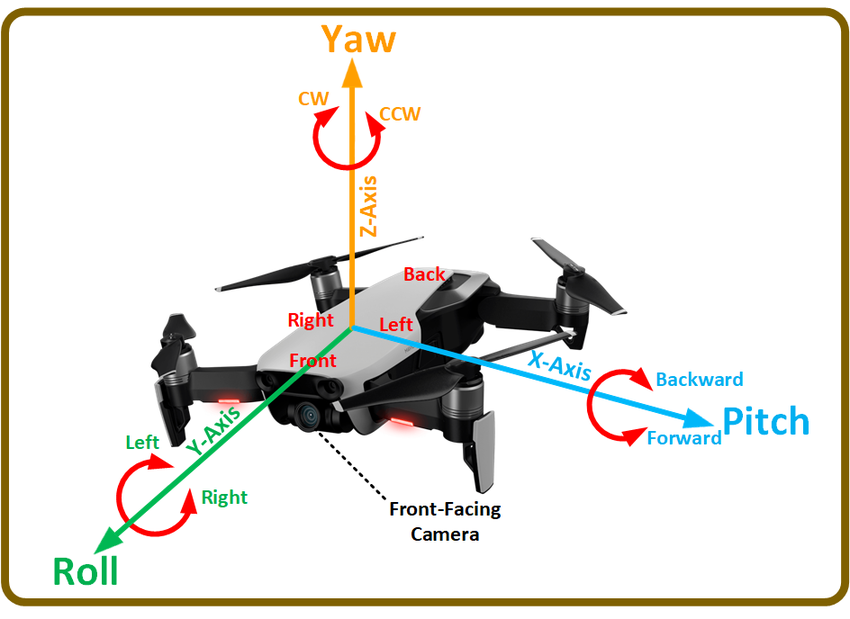
\includegraphics[width=0.7\textwidth]{Figures/Chapter1/Section2/1.png} 
        \caption{  Principal Movements of a UAV in 3D Space (adapted from: \cite{almahamid2024viznav})}
        \label{fig:method3_architecture} % Reference label
    \end{figure}


% These movements are essential for UAVs to navigate through their environment, maintain stability, and complete missions effectively. The ability to control these movements accurately is vital for ensuring the success of UAV operations, especially in dynamic and complex environments.

\vspace{0.5cm}

The characteristics of UAVs-such as speed, flight time, payload capacity, range, altitude, and principal movements are fundamental to their overall design and performance. Each characteristic impacts the UAV's ability to carry out specific tasks, whether it's surveillance, communication, or commercial applications. Understanding and optimizing these factors is essential for advancing UAV technology and ensuring the successful deployment of UAVs across various industries. As research continues to improve UAV designs, advancements in battery life, payload efficiency, and flight stability are expected to enhance the capabilities of UAVs, enabling them to perform more complex and longer-duration missions.


%%%%%%%%%%%%%%%%%%%%%%%%%%%%%%%%%%%%%%%%%%%%%%%%%%%%%%%%%%%%%%%%%%%%%%
%%%%%%%%%%%%%%%%%%%%%%%%%%%%%%%%%%%%%%%%%%%%%%%%%%%%%%%%%%%%%%%%%%%%%%
%%%%%%%%%%%%%%%%%%%%%%%%%%%%%%%%%%%%%%%%%%%%%%%%%%%%%%%%%%%%%%%%%%%%%%


\section{Communication protocols for UAVs}

Communication between the UAV and the Ground Control Station (GCS) relies on established communication protocols. However, existing protocols are not well-suited to the UAV environment. Due to the limited resources and the highly dynamic nature of unmanned systems, these protocols often fail to function efficiently according to \cite{larrieu2014model}.

\vspace{0.5cm}

This issue becomes even more critical when considering security measures, as UAVs typically operate with constraints such as limited battery life, restricted real-time processing power, and autonomous control requirements. Limited energy resources, communication bandwidth, and computational capacity make traditional protocols like TLS and Kerberos impractical for UAV networks.

\vspace{0.5cm}

Various communication protocols have been specifically developed for Unmanned Aerial Vehicles (UAVs). In this section, we will discuss these protocols in detail.


\subsection{UranusLink Protocol}


 UranusLink supports both unreliable and reliable packet‑oriented communication, defining the packet structure and the format in which data is transmitted. The protocol’s overall mechanism and detailed description are provided by Kriz et al.~\cite{kriz2015uranuslink}. In this study, we adopt their packet structure, as illustrated in Table~\ref{tab:uranuslink_pivoted}. Each packet comprises six fields: \textbf{Preamble} (PRE), \textbf{Sequence Number} (SQN), \textbf{Message Identification} (MID), \textbf{Data Length} (LEN), \textbf{Data}, and \textbf{Checksum} (CS).



\begin{table}[h]
\centering
\begin{tabular}{|c|c|c|c|c|c|c|}
\hline
\textbf{PRE} & \textbf{SQN} & \textbf{MID} & \textbf{LEN} & \textbf{DATA} & \textbf{CS} \\
\hline
1 B & 2 B & 1 B & 1 B & 1–252 B & 1 B \\
\hline
\end{tabular}
\caption{UranusLink packet structure. (adapted from \cite{kriz2015uranuslink})}
\label{tab:uranuslink_pivoted}
\end{table}

The UranusLink protocol is tailored for radio communications, where data loss and corruption are frequent.  Each packet begins with a \textbf{preamble (PRE)} byte \texttt{0xFD}, which seldom occurs in payloads, ensuring reliable packet boundary detection.  Following this is an even-valued \textbf{sequence number (SQN)}, used to detect lost or out of order packets any packet with an SQN lower than the last accepted is discarded and a \textbf{checksum (CS)} to validate integrity.  The sizes of PRE and CS balance robustness against overhead, taking link conditions and capacity into account.

\vspace{0.5cm}

The \textbf{MID} field specifies how to interpret the payload.  Currently there are eight UAV to ground and sixteen ground‑to‑UAV message types; the two critical ones establish and maintain the connection in each direction.  

\vspace{0.5cm}

Two UAV modes are supported: \textbf{flight mode}, in which the rotors spin, and \textbf{configuration mode}, used on the ground.  A “robot mode switch” message triggers transitions, and only these mode‑switch packets are acknowledged other messages are sent unacknowledged to minimize overhead.  The ground station tracks SQNs of mode switch requests so it can determine the UAV’s current mode even if acknowledgments are lost.

\vspace{0.5cm}

Compared to MAVLink which can incur up to 33 \% extra overhead and offers no built‑in security UranusLink achieves much lower overhead while providing essential reliability and mode‑switch acknowledgment.



\subsection{UAVCAN protocol}

UAVCAN is an open‑source, masterless publish–subscribe protocol for secure connectivity over CAN buses in aerospace and robotics.  It carries long payloads in a single CAN frame (e.g.\ GNSS fixes, 3D vectors), supports multiple nodes and interfaces for high‑safety applications, and offers standard services such as network discovery, node configuration and firmware upgrade, status monitoring, time synchronization, and adaptive node‑ID allocation.  Lightweight and real‑time–capable, UAVCAN is ideal for resource‑constrained UAVs and is released under the MIT license \cite{kriz2015uranuslink}.

\vspace{0.5cm}

Based on the CAN bus, originally created for automotive multiplex wiring, UAVCAN enables host‑free communication between devices and microcontrollers \cite{kriz2015uranuslink}.  Each node is assigned a unique ID in the range 1–127 (ID 1 typically denotes the autopilot; 126–127 are for debugging).  To avoid mismatches, any MAVLink component communicating over UAVCAN must use the same Component ID (COMPID) as its UAVCAN Node ID commonly both set to 1 so that every MAVLink message’s COMPID field matches its UAVCAN node ID \cite{kriz2015uranuslink}.




\subsection{MAVLink protocol}


MAVLink is an open and efficient communication protocol tailored for lightweight, real-time interactions between Unmanned Aerial Vehicles (UAVs) and Ground Control Stations (GCSs). Developed by Lorenz Meier and first released in 2009 under the LGPL license, MAVLink 1.0 quickly became popular thanks to its streamlined design and operational simplicity \cite{allouch2019mavsec, koubaa2017mavlink}. A significant evolution of the protocol occurred in 2017 with the introduction of MAVLink 2.0, which is currently the preferred version. It maintains backward compatibility with MAVLink 1.0 while offering improvements in extensibility, robustness, and security features.

\vspace{0.5cm}

MAVLink messages are broadly categorized into two types: those originating from the GCS to issue commands or control instructions to UAVs, and those transmitted by UAVs to the GCS, typically conveying telemetry data such as geographical coordinates, altitude, system heartbeat, and operational status. To meet the demands of real-time systems, MAVLink was designed with minimal communication overhead to ensure high efficiency \cite{allouch2019mavsec}. The following sections provide a comparative overview of the header structures used in MAVLink 1.0 and its successor, MAVLink 2.0.



\subsubsection{MAVLink 1.0 header protocol}


The comprehensive survey by Koubaa et al. \cite{koubaa2017mavlink} remains the only detailed study focused on the MAVLink protocol’s architecture and operational principles. As part of their contribution, the authors present the header structure for MAVLink 1.0. Below, we describe the structure of a MAVLink 1.0 frame, which consists of eight primary fields, as illustrated in Figure~\ref{fig:mavlink-v1-packet}.

The first byte, labeled \textbf{STX}, has a fixed value of \texttt{0xFE}, which identifies the start of a MAVLink 1.0 message frame. The second field, \textbf{LEN}, encoded in one byte, indicates the length of the payload. The third field, \textbf{SEQ}, is also one byte and stores a sequence number ranging from 0 to 255. Once 255 is reached, it rolls over to 0. This sequence number helps in detecting lost packets.

To distinguish between multiple UAVs managed by a single Ground Control Station, the fourth field, \textbf{SYS ID}, is used. This field also spans one byte, limiting the addressable systems to 254 UAVs, since ID 255 is typically reserved for the GCS. The fifth field, \textbf{COMP ID}, identifies the specific component (e.g., autopilot, gimbal) transmitting the message. Finally, the sixth byte marks the beginning of the payload section, which contains the message-specific data.

\begin{figure}[ht]
\centering
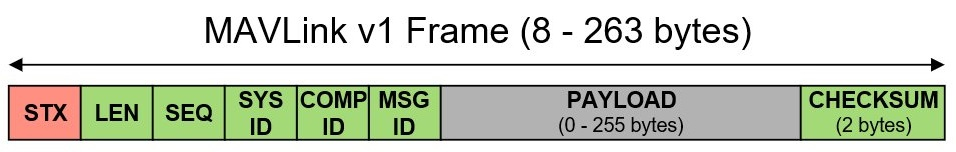
\includegraphics[width=0.9\textwidth]{Figures/Chapter1/Section4/1.jpg} % Save image locally
\caption{Structure of a MAVLink 1.0 packet \cite{mavlinkio}.}
\label{fig:mavlink-v1-packet}
\end{figure}





\begin{table}[ht]
\renewcommand{\arraystretch}{1.3} % Slightly more vertical space for centering
\centering
\caption{MAVLink 1.0 header structure and byte size. (adapted from \cite{koubaa2017mavlink})}
\begin{tabular}{|>{\centering\arraybackslash}m{2.5cm}|
                >{\centering\arraybackslash}m{2cm}|
                >{\arraybackslash}m{7cm}|}
\hline
\textbf{Field} & \textbf{Size} & \textbf{Description} \\
\hline
STX & 1 B & \vspace{0pt}Start-of-frame indicator (0xFE in MAVLink 1.0). \\
\hline
LEN & 1 B & \vspace{0pt}Payload length (0–255 bytes). \\
\hline
SEQ & 1 B & \vspace{0pt}Packet sequence number (0–255, wraps after 255). Used to detect packet loss. \\
\hline
SYS ID & 1 B & \vspace{0pt}System identifier (e.g., UAV ID). Value 255 is typically used by the GCS. \\
\hline
COMP ID & 1 B & \vspace{0pt}Component identifier (e.g., autopilot or camera module). \\
\hline
Message ID & 1 B & \vspace{0pt}Indicates the type of MAVLink message. \\
\hline
Payload & 0–255 B & \vspace{0pt}Actual message data depending on message type. \\
\hline
Checksum (CRC) & 2 B & \vspace{0pt}Verifies the integrity of the packet (LSB to MSB order). \\
\hline
\end{tabular}
\label{tab:mavlink_header}
\end{table}





In summary, the MAVLink 1.0 protocol employs a lightweight and efficient packet structure that balances low bandwidth usage with sufficient message integrity. The use of fixed-length headers, flexible payloads up to 255 bytes, and a robust CRC-based checksum mechanism ensures reliable communication between UAVs and ground stations. Understanding the role of each header field, especially the \texttt{Message ID}, is essential for correctly interpreting messages and extracting relevant data from the payload.



\subsubsection{MAVLink 2.0 Protocol}

MAVLink 2.0 was introduced in early 2017 \cite{allouch2019mavsec, khan2020emerging}, offering enhancements over MAVLink 1.0 while maintaining backward compatibility. This section presents the MAVLink 2.0 header structure and compares it with MAVLink 1.0. The MAVLink 2.0 header is shown in Fig.~\ref{fig:mavlink-v2-packet}, and Table~\ref{tab:mavlink2_additional_fields} explains the additional fields in the MAVLink 2.0 header compared to MAVLink 1.0.

\vspace{0.5cm}

MAVLink 2.0 retains all fields from MAVLink 1.0 but adds new fields and expands some existing ones. The first byte (0xFD) marks the start of the message, differing from MAVLink 1.0's 0xFE. The payload length field remains unchanged. Two flags appear before the sequence number (SEQ): the incompatibility flag, which indicates if the packet is signed, and the compatibility flag, which does not affect the message structure.

\begin{figure}[ht]
\centering
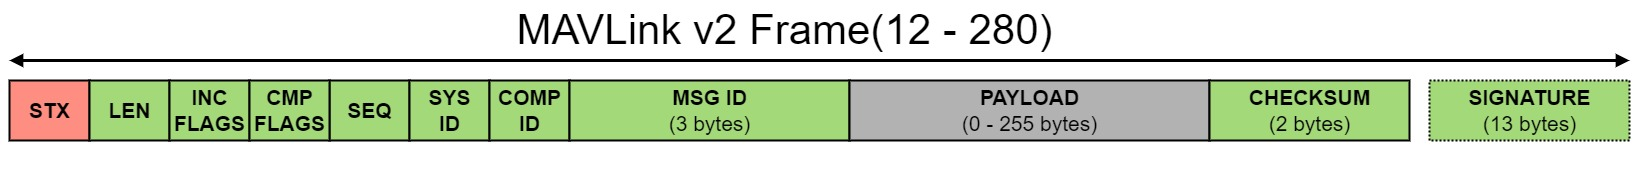
\includegraphics[width=0.8\textwidth]{Figures/Chapter1/Section4/2.jpg}
\caption{MAVLink 2.0 Header Structure.}
\label{fig:mavlink-v2-packet}
\end{figure}


\begin{table}[H]
\renewcommand{\arraystretch}{1.3} % Slightly more vertical space for centering
\centering
\caption{Additional MAVLink 2.0 Header Fields (compared to MAVLink 1.0).}
\begin{tabular}{|>{\centering\arraybackslash}m{2.5cm}|
                >{\centering\arraybackslash}m{2cm}|
                >{\arraybackslash}m{7cm}|}
\hline
\textbf{Field} & \textbf{Size} & \textbf{Description} \\
\hline
STX & 1 B & \vspace{0pt}Start-of-frame indicator (0xFD in MAVLink 2.0). \\
\hline
Incompatibility Flag & 1 B & \vspace{0pt}Indicates whether the message is signed (e.g., 0x01 indicates signed message). \\
\hline
Compatibility Flag & 1 B & \vspace{0pt}Indicates compatibility options that can be ignored by parsers if not recognized. \\
\hline
MSGID & 3 B & \vspace{0pt}Message identifier, expanded from 8 bits in MAVLink 1.0 to 24 bits in MAVLink 2.0, allowing up to 16,777,215 different message types. \\
\hline
Signature & 13 B & \vspace{0pt}Used for message authentication, ensuring integrity and authenticity, including LinkID, Timestamp, and the actual Signature field. \\
\hline
\end{tabular}
\label{tab:mavlink2_additional_fields}
\end{table}

The SEQ (sequence number), system ID, and COMPID fields in MAVLink 2.0 are identical to those in MAVLink 1.0. The MSGID field is expanded from 8 to 24 bits, increasing the number of possible messages to over 16 million. The payload field can carry up to 255 bytes. The checksum in MAVLink 2.0 remains the same as in MAVLink 1.0.

\vspace{0.5cm}

MAVLink 2.0 introduces a 13-byte field for message authentication, improving security over MAVLink 1.0. The message signature is appended when the incompatibility flag is set to 0x01. This addition significantly enhances security by ensuring message integrity and authenticity.

\vspace{0.5cm}

The 13-byte message signature contains the following fields:
\begin{itemize}
    \item \textbf{LinkID:} A one-byte field representing the link (channel) used to send the packet. The link refers to any telemetry device (e.g., Wi-Fi). Each channel used to send information has a unique LinkID.
    \item \textbf{Timestamp:} Encoded as 6 bytes in 10-microsecond units, the timestamp represents the time since January 1, 2015 GMT. The timestamp increases with each message sent over the channel and helps prevent replay attacks.
    \item \textbf{Signature:} This field covers the full message, the secret key, and the timestamp. It is encrypted into 6 bytes for the message. The first 6 bytes (48 bits) of a SHA-256 hash applied to the MAVLink 2.0 message are included in the signature. A 32-byte shared symmetric key is stored on both ends, i.e., the autopilot and the ground station or the MAVLink API.
\end{itemize}

Messages are discarded if: (1) they are received earlier than a previous packet from the same tuple (LinkID, SystemID, ComponentID); (2) the signature does not match; or (3) the timestamp exceeds one minute compared to the local system time \cite{koubaa2017mavlink}.




\subsection{ Disscussion}


UAV operations depend critically on communication protocols that remain vulnerable despite widespread use. Current protocols like MAVLink, UranusLink, and UAVCan (compared in Table~\ref{tab:uav_protocol_comparison}) each compromise between functionality, maturity, and crucial security features.




\begin{table}[H]
\centering
\renewcommand{\arraystretch}{1.0} % Reduced from 1.3
\setlist[itemize]{nosep,leftmargin=*,topsep=0pt,partopsep=0pt} % Compact lists
\begin{tabular}{|>{\centering\arraybackslash}m{3cm}|
                >{\arraybackslash}m{6cm}|
                >{\arraybackslash}m{6cm}|}
\hline
\textbf{Protocol} & \textbf{Pros} & \textbf{Limitations} \\ 
\hline
UranusLink & 
\begin{itemize}
    \item Open-source
    \item Lightweight
    \item Aerospace/robotic focus
    \item Redundant transports
\end{itemize} & 
\begin{itemize}
    % \item Unstable version
    \item Limited language support
    \item No concurrency
    \item Not scalable
    \item Lacks security
\end{itemize} \\ 
\hline
UAVCan & 
\begin{itemize}
    \item Open-source
    \item Lightweight
    \item Low latency
    \item Data loss recovery
\end{itemize} & 
\begin{itemize}
    \item Limited language support
    \item No concurrency
    \item Not scalable
\end{itemize} \\ 
\hline
MAVLink & 
\begin{itemize}
    \item Widely accepted
    \item Scalable
    \item Multi-language
    \item Concurrent systems
    \item Proven performance
\end{itemize} & 
\begin{itemize}
    \item No payload security
    \item Weak encryption
    \item Small data only
    \item Open format
\end{itemize} \\ 
\hline
\end{tabular}
\caption{Comparison of UAV Communication Protocols}
\label{tab:uav_protocol_comparison}
\end{table}





As evidenced in Table~\ref{tab:uav_protocol_comparison}, current UAV protocols prioritize lightweight operation and low latency at the expense of robust security - particularly MAVLink, whose widespread use in critical operations contrasts sharply with its lack of payload encryption and authentication \cite{khan2020emerging}. These security gaps create attack vectors for message spoofing, data interception, and even UAV hijacking, with potentially catastrophic consequences for sensitive operations ranging from military reconnaissance to emergency response missions. The protocol limitations underscore an urgent need for security-enhanced communication frameworks that maintain performance while addressing these vulnerabilities.






%%%%%%%%%%%%%%%%%%%%%%%%%%%%%%%%%%%%%%%%%%%%%%%%%%%%%%%%%%%%%%%%%%%%%%
%%%%%%%%%%%%%%%%%%%%%%%%%%%%%%%%%%%%%%%%%%%%%%%%%%%%%%%%%%%%%%%%%%%%%%
%%%%%%%%%%%%%%%%%%%%%%%%%%%%%%%%%%%%%%%%%%%%%%%%%%%%%%%%%%%%%%%%%%%%%%


\section{UAVs Architectures}



The communication architecture is essential for enabling intelligent control and autonomous collaboration in UAV swarms. Initially, centralized architectures an extension of traditional single-UAV systems were used, with a single ground station managing all UAV communication. However, as swarm size and mission complexity grew, decentralized architectures emerged as more scalable alternatives, reducing dependency on central nodes \cite{Cao2012}. Many studies have since explored different swarm communication models. This section reviews the main architectures, summarizing their characteristics, strengths, and limitations.




%%%%%%%%%%%%%%%%%%%%%%%%%%%%%%%%%%%%%%%%%%%%%%%%%%%%%%%%%%%%%%%%%%%%%%


\subsection{Centralized Communication Architecture}
\label{sec:centralized}

The \textbf{centralized communication architecture}, adapted from single-UAV systems, was later applied to UAV swarms. As shown in \textbf{Figure~\ref{fig:centralized communication architecture}}, it relies on a central node, such as fixed network infrastructure, connecting all UAVs through direct one-to-one links without intermediary relays. This setup offers routing simplicity, stability, and efficient performance at small scales. It is best suited for missions with limited swarm size, coverage, and complexity. A notable implementation is the \textbf{"UAV-GCS Centralized Data-Oriented Communication Architecture"} used in crowd surveillance \cite{Chen2020}.


\begin{figure}[H]
\centering
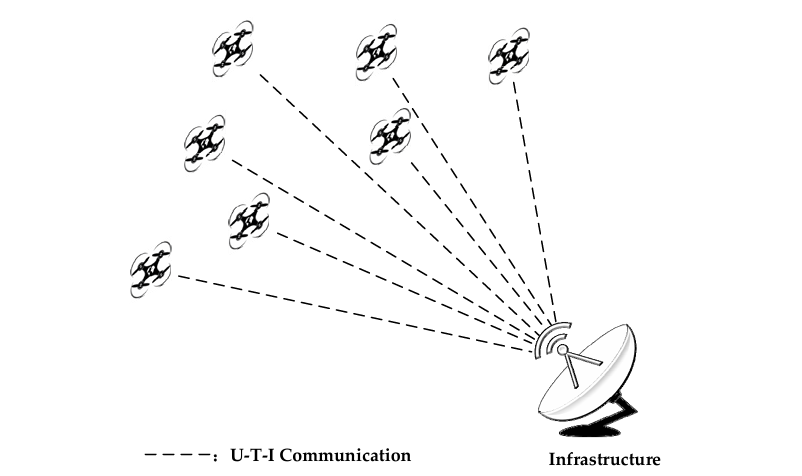
\includegraphics[width=0.8\textwidth]{Figures/Chapter1/Section5/1.png}
\caption{centralized communication architecture \cite{Chen2020}}
\label{fig:centralized communication architecture}
\end{figure}

Despite its simplicity, this architecture presents key limitations. All inter-UAV communication must pass through the infrastructure, making the \textbf{UAV-to-Infrastructure (U-T-I)} distance typically longer than the \textbf{UAV-to-UAV (U-T-U)} distance, resulting in increased latency. Moreover, the high mobility of UAVs and growing coverage requirements render the system unstable. A major weakness is its \textbf{Single Point of Failure (SPOF)} if the ground station or satellite fails, the entire network collapses. As a result, centralized architectures are unsuitable for large-scale or high-risk missions.



%%%%%%%%%%%%%%%%%%%%%%%%%%%%%%%%%%%%%%%%%%%%%%%%%%%%%%%%%%%%%%%%%%%%%%


\subsection{Decentralized Communication Architecture}

Given the high operational speeds of UAVs and the extensive coverage demands of missions, network connectivity often fluctuates as UAVs dynamically join and leave the network. This variability makes ad hoc networking ideal for UAV swarms. In decentralized architectures, UAVs establish real-time, self-organizing connections, eliminating the need for fixed infrastructure and overcoming traditional communication range limitations \cite{Chen2020}.



\subsubsection{Single-Group Swarm Ad Hoc Network}

In a single-group swarm ad hoc network (~\ref{fig:single-group_swarm_Ad_hoc_network}), communication occurs independently of fixed infrastructure, with a gateway UAV linking the swarm to external systems and other UAVs acting as relay nodes to distribute data. This structure supports real-time information sharing among swarm members, improving operational efficiency. The gateway UAV uses two transceivers: a short-range, low-power unit for intra-swarm communication and a long-range, high-power system for external links \cite{Chen2020}. This design enables the use of lightweight transceivers in regular UAVs, extending coverage and accommodating smaller UAVs. However, the system requires uniform flight patterns, making it well-suited for homogeneous small UAV groups. When applied to heterogeneous swarms with different UAV types, variations in operational characteristics prevent close formation flying, leading to the development of more adaptable multi-group and multi-layer architectures for complex mission needs.


\begin{figure}[ht]
\centering
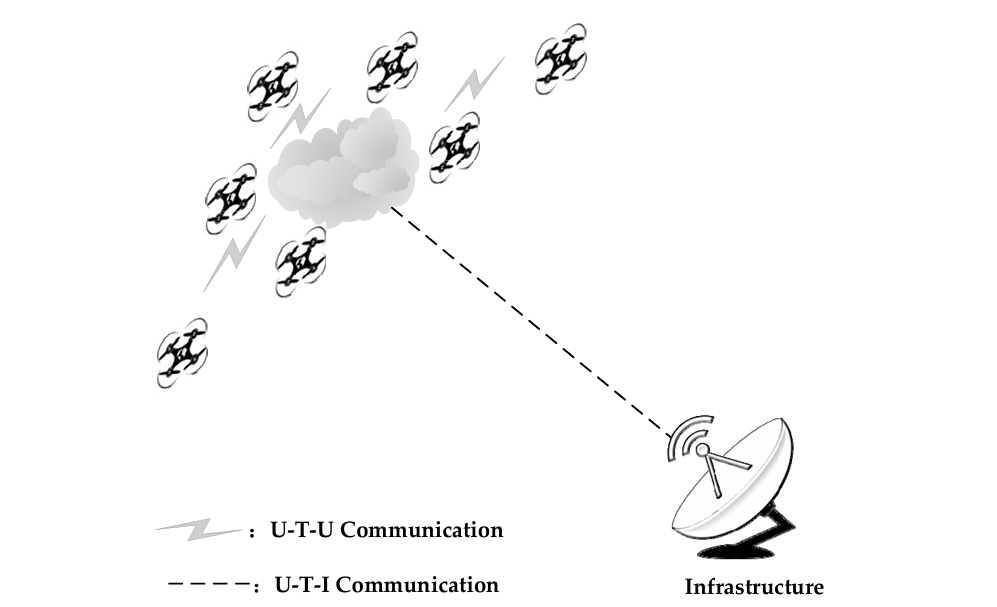
\includegraphics[width=0.8\textwidth]{Figures/Chapter1/Section5/2.png}
\caption{single-group swarm Ad hoc network \cite{Chen2020}}
\label{fig:single-group_swarm_Ad_hoc_network}
\end{figure}


% \vspace{0.5cm}

Several intra-swarm communication  configurations (~\ref{fig:intra-swarm communication architecture}) have emerged:
\begin{itemize}
\item \textbf{Ring Architecture}: Forms a closed communication loop where any UAV can serve as gateway, providing redundancy but limited scalability
\item \textbf{Star Architecture}: Centralizes communication through a gateway UAV, creating a single point of failure vulnerability
\item \textbf{Meshed Architecture}: Combines ring and star advantages, allowing any UAV to function as a gateway with multiple routing paths
\end{itemize}

While meshed architecture has become the standard for its flexibility, mission diversity increasingly requires swarms to incorporate varied UAV sizes and capabilities, pushing the development of more advanced network topologies.





\begin{figure}[ht]
\centering
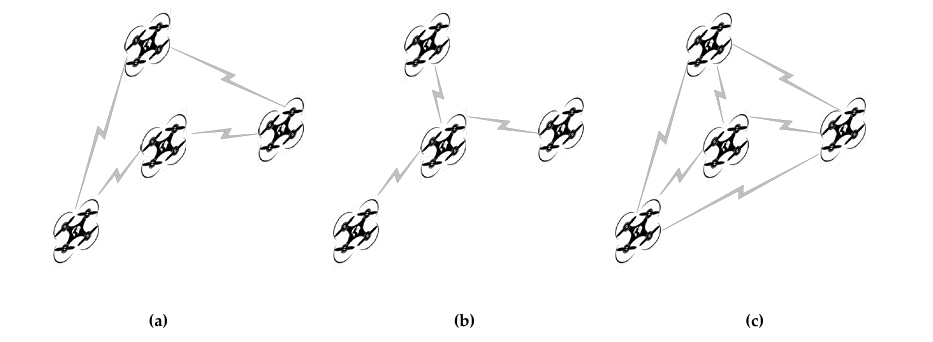
\includegraphics[width=0.7\textwidth]{Figures/Chapter1/Section5/3.png}
\caption{intra-swarm communication architecture: (a): ring rchitecture, (b) star architectue, (c): meshedarchitecture. \cite{Chen2020}}
\label{fig:intra-swarm communication architecture}
\end{figure}


\subsubsection{Multi-Group Swarm Ad hoc Network}

The \textit{multi-group swarm Ad hoc network} (Figure~\ref{fig:multi-group swarm Ad hoc network}) combines elements of both centralized and \textit{single-group swarm Ad hoc network} architectures to address the limitations of the latter. Each group, depending on its mission, operates in an Ad hoc manner for intra-group communication, while inter-group communication (Group-to-Group or G-T-G) relies on the infrastructure, with gateway UAVs handling communication with the central infrastructure. This architecture is semi-centralized, and while it can accommodate diverse UAV types for complex missions, it still suffers from high latency in G-T-G communications. The \textit{multi-group swarm Ad hoc network} is particularly suitable for applications like multi-theater joint operations in military scenarios, where a central control center coordinates UAV swarms that approach the mission area from various directions~\cite{kaleem2019uav}.


\begin{figure}[ht]
\centering
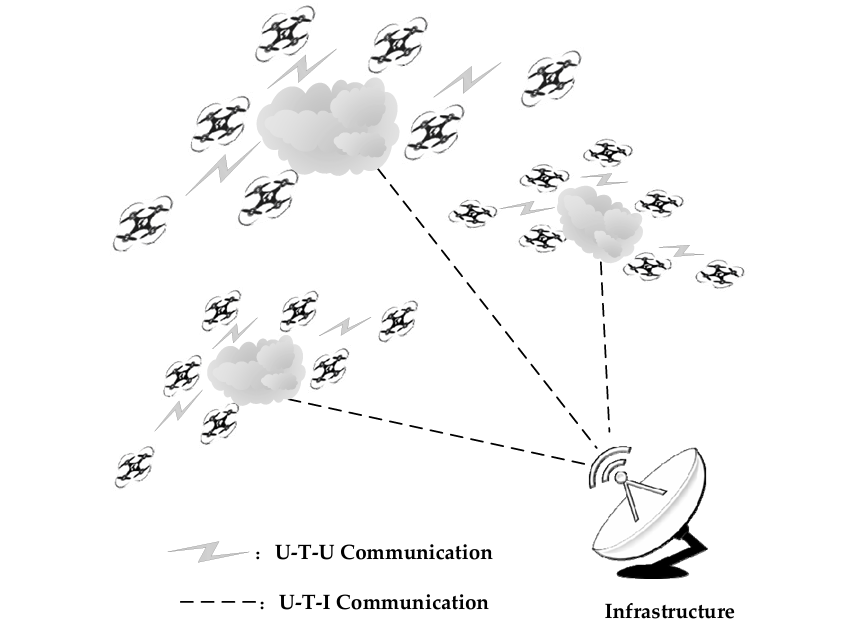
\includegraphics[width=0.6\textwidth]{Figures/Chapter1/Section5/4.png}
\caption{multi-group swarm Ad hoc network \cite{Chen2020}}
\label{fig:multi-group swarm Ad hoc network}
\end{figure}



\subsubsection{Multi-layer Swarm Ad hoc Network}


The \textit{multi-layer swarm Ad hoc network} architecture, as depicted in Figure~\ref{fig:multi-layer swarm Ad hoc network}, is a more advanced version of the \textit{multi-group swarm Ad hoc network}. In this architecture, UAVs of the same type form an Ad hoc network at the first layer, enabling intra-group communication. At the second layer, gateway UAVs facilitate Group-to-Group (G-T-G) communication between different UAV groups. The third layer consists of the gateway UAVs communicating with the infrastructure. Notably, UAVs in the same group can communicate directly without infrastructure relay, while inter-group communication passes through the gateway UAV \cite{Chen2020} Data packets move through the first and second layers sequentially, ensuring there is no single point of failure (SPOF). This multi-layer structure offers increased robustness compared to other architectures.


\begin{figure}[ht]
\centering
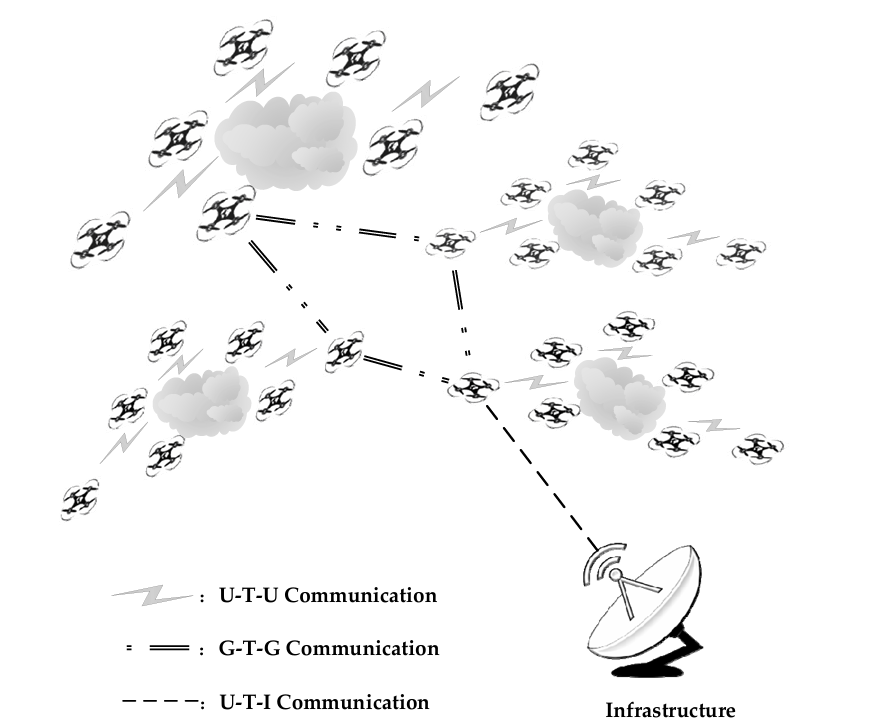
\includegraphics[width=0.6\textwidth]{Figures/Chapter1/Section5/5.png}
\caption{multi-layer swarm Ad hoc network \cite{Chen2020}}
\label{fig:multi-layer swarm Ad hoc network}
\end{figure}


The \textit{multi-layer swarm Ad hoc network} architecture adapts to changes in UAV numbers, enabling quick network reconstruction. It is ideal for complex missions with dynamic network topologies and frequent UAV communication. Future improvements may include adding more layers to enhance task coverage and network robustness.


%%%%%%%%%%%%%%%%%%%%%%%%%%%%%%%%%%%%%%%%%%%%%%%%%%%%%%%%%%%%%%%%%%%%%%


\subsection{Discussion}


UAV swarm communication architecture has advanced significantly, with various options for different mission scenarios. Centralized architecture suits small, simple missions with long-range communication to infrastructure \cite{Chen2020}. Decentralized architecture extends coverage via multi-hop networks and gateway UAVs for UAV-to-infrastructure communication. The \textit{single-group swarm Ad hoc network} works for homogenous UAVs, while the \textit{multi-group} and \textit{multi-layer swarm Ad hoc network} architectures are better for diverse UAV types, though the former may face delays in inter-group communication. The \textit{multi-layer swarm Ad hoc network} is more robust, eliminating single point of failure (SPOF).




\begin{table}[H]
\centering
\renewcommand{\arraystretch}{1.0}
\setlist[itemize]{nosep,leftmargin=*,topsep=0pt,partopsep=0pt}
\begin{tabular}{|>{\centering\arraybackslash}m{3.5cm}|
                >{\centering\arraybackslash}m{2.2cm}|
                >{\centering\arraybackslash}m{2.2cm}|
                >{\centering\arraybackslash}m{2.2cm}|
                >{\centering\arraybackslash}m{2.2cm}|
                >{\centering\arraybackslash}m{2.2cm}|}
\hline
\textbf{Features} & \textbf{Centralized} & \textbf{Decentralized} & \textbf{Single-Group} & \textbf{Multi-Group} & \textbf{Multi-Layer} \\
\hline
Multi-hop Communication & x & \checkmark & \checkmark & \checkmark & \checkmark \\
\hline
UAVs Relay Traffic      & x & \checkmark & \checkmark & \checkmark & \checkmark \\
\hline
Different Types of UAVs & x & \checkmark & x & \checkmark & \checkmark \\
\hline
Self-configuration      & x & \checkmark & \checkmark & \checkmark & \checkmark \\
\hline
Limited Coverage        & \checkmark & x & x & x & x \\
\hline
Single Point of Failure & \checkmark & x & x & x & x \\
\hline
Robustness              & x & \checkmark & \checkmark & \checkmark & \checkmark \\
\hline
\end{tabular}
\caption{Summary of UAV Swarm Communication Architectures (\checkmark = supported, x = not supported) \cite{Chen2020}}
\label{tab:swarm_architecture_summary}
\end{table}


UAV swarm communication architectures must balance high coverage and connectivity. Coverage is key for intelligence gathering, while connectivity ensures real-time communication. However, dynamic environments make maintaining connectivity challenging due to signal attenuation. To avoid disruption, UAVs must stay within a suitable distance for effective communication. Nature-inspired behaviors can improve positioning, and advancements in 4G and 5G networks offer potential solutions for better connectivity across wide areas.



%%%%%%%%%%%%%%%%%%%%%%%%%%%%%%%%%%%%%%%%%%%%%%%%%%%%%%%%%%%%%%%%%%%%%%
%%%%%%%%%%%%%%%%%%%%%%%%%%%%%%%%%%%%%%%%%%%%%%%%%%%%%%%%%%%%%%%%%%%%%%
%%%%%%%%%%%%%%%%%%%%%%%%%%%%%%%%%%%%%%%%%%%%%%%%%%%%%%%%%%%%%%%%%%%%%%


\section{Routing Protocols}


This section reviews common UAV swarm communication routing technologies, classifies routing protocols based on their underlying techniques, and provides a detailed overview of each category, highlighting their pros and cons. Building on prior comparisons of current architectures where the multi-layer swarm Ad hoc network showed the best overall performance it emphasizes the critical role of routing in ensuring reliable U-T-U communication, despite challenges like UAV mobility, unstable links, limited resources, and varying QoS needs. Traditional Ad hoc protocols require adaptation, making the design of suitable routing protocols a key research focus.


%%%%%%%%%%%%%%%%%%%%%%%%%%%%%%%%%%%%%%%%%%%%%%%%%%%%%%%%%%%%%%%%%%%%%%

\subsection{Routing Technologies}

Routing technologies form the foundation for implementing routing protocols, which are often built by enhancing or combining these basic techniques. Since UAV swarm Ad hoc networks evolve from traditional Ad hoc networks, conventional routing methods can still be applied after suitable analysis and adaptation. The six common routing technologies used include store-carry-forward, greedy forwarding, path discovery, single-path, multi-path, and predictive routing \cite{Chen2020}.


\begin{figure}[ht]
\centering
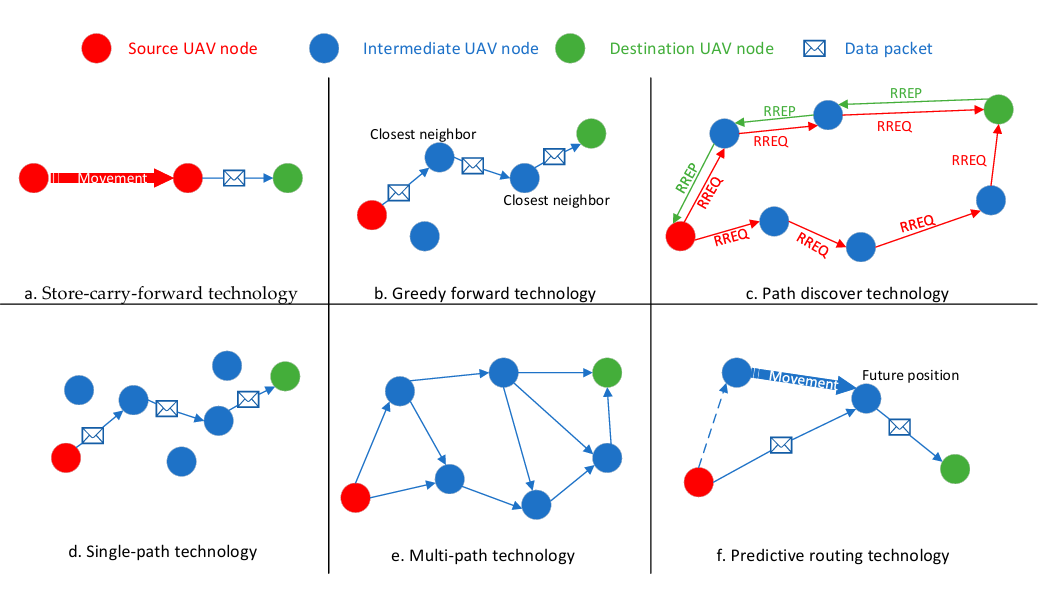
\includegraphics[width=0.9\textwidth]{Figures/Chapter1/Section6/1.png}
\caption{The rationales for common routing technologies of UAV ad hoc network.\cite{Chen2020}.}
\label{fig:The rationales for common routing technologies of UAV ad hoc network.}
\end{figure}



\begin{enumerate}
    \item \textbf{Store-carry-forward:} When no relay is available, the node stores and carries the data until it finds one. Suitable for intermittent networks but causes high delays.

    \item \textbf{Greedy forward:} Selects the neighbor closest to the destination as the next hop. Works well in dense UAV deployments but may fail if no closer neighbor exists requiring backup strategies.

    \item \textbf{Path discovery:} Uses flooding (RREQ) to find routes, improving path availability when location info is lost. However, it consumes significant bandwidth.

    \item \textbf{Single-path:} Sends data through one route, conserving bandwidth but lacking robustness no backup path if a failure occurs.

    \item \textbf{Multi-path:} Maintains several routes to improve reliability. If one path fails, others can take over. However, shared path failures can cause loops.

    \item \textbf{Predictive routing:} Estimates future positions based on current motion to choose the next hop. Ideal for high-mobility UAV swarms.
\end{enumerate}



%%%%%%%%%%%%%%%%%%%%%%%%%%%%%%%%%%%%%%%%%%%%%%%%%%%%%%%%%%%%%%%%%%%%%%

\subsection{The Classification of Routing Protocols}

Early research on UAV swarm communication focused on adapting traditional Ad hoc routing protocols. However, these proved largely unsuitable due to the unique characteristics of UAVs such as high mobility and varying mission requirements. As a result, researchers both enhanced existing protocols and developed new ones specifically for UAV swarms \cite{koubaa2017mavlink, Chen2020}. These routing protocols are now broadly categorized into three main types, each with several subtypes, as shown in ~\ref{fig:routing-protocols-classification}

\begin{figure}[ht]
\centering
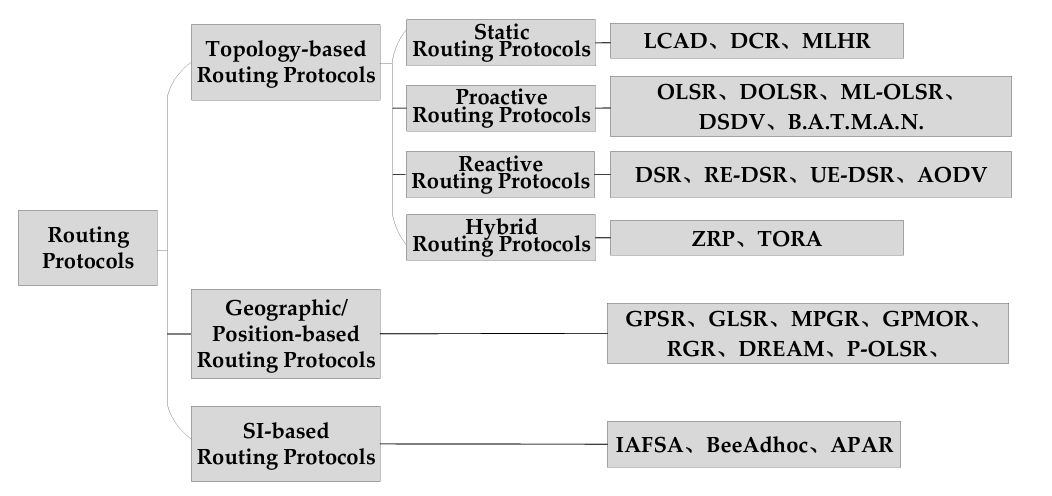
\includegraphics[width=0.7\textwidth]{Figures/Chapter1/Section6/2.png}
\caption{Classification of all routing protocols \cite{Chen2020}.}
\label{fig:routing-protocols-classification}
\end{figure}


%%%%%%%%%%%%%%%%%%%%%%%%%%%%%%%%%%%%%%%%%%%%%%%%%%%%%%%%%%%%%%%%%%%%%%

\subsection{Topology-Based Routing Protocols}

Topology-based routing protocols rely on IP addresses and known link information to forward packets efficiently. They are typically categorized into static, proactive, reactive, and hybrid protocols.

\subsubsection{Static Routing Protocols}


Static routing protocols use fixed routing tables and are suitable for stable topologies without task updates. Due to their lack of adaptability, their use in dynamic UAV swarms is limited. Notable examples include:

\begin{itemize}
    \item \textbf{Load Carry and Deliver (LCAD)}: Proposed by Le et al., LCAD uses a centralized system where a UAV carries and delivers data to its destination. It maximizes throughput and reduces hops but suffers from significant delays with increased communication distance.
    
    \item \textbf{Data Centric Routing (DCR)}: Designed for one-to-many transmission, DCR works well in “single-group swarm Ad hoc networks” with a gateway UAV distributing information. It’s ideal for small, planned UAV networks with minimal coordination between nodes.
    
    \item \textbf{Multilevel Hierarchical Routing (MLHR)}: Derived from vehicular networks, MLHR organizes UAVs into hierarchical layers, with gateway UAVs handling group-to-group communication ~\ref{fig:Multilevel Hierarchical Routing in a UAV swarm Ad hoc network}. It improves scalability and communication efficiency through geographic clustering.
\end{itemize}


\begin{figure}[ht]
\centering
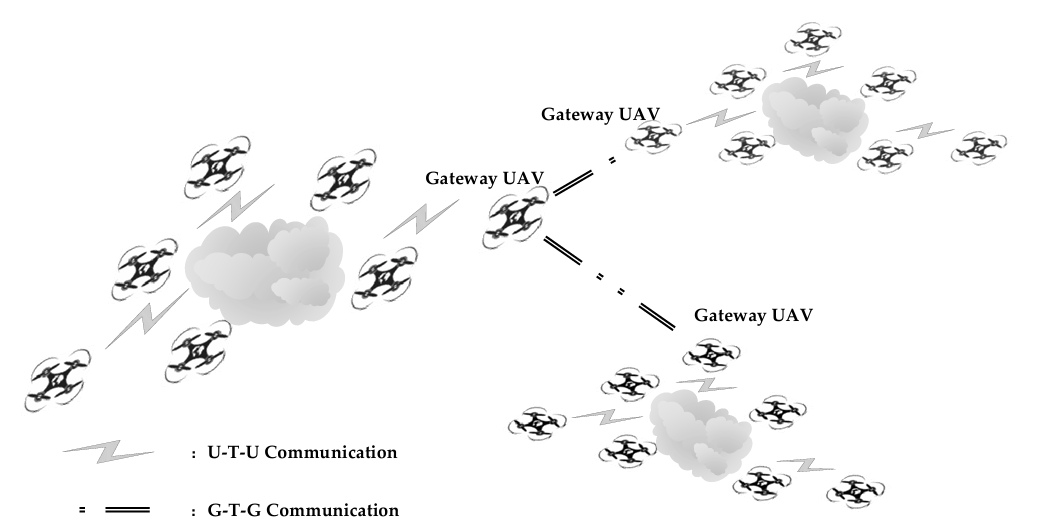
\includegraphics[width=0.7\textwidth]{Figures/Chapter1/Section6/3.png}
\caption{Multilevel Hierarchical Routing in a UAV swarm Ad hoc network}
\label{fig:Multilevel Hierarchical Routing in a UAV swarm Ad hoc network}
\end{figure}


\subsubsection{Proactive Routing Protocols}


Proactive routing protocols (PRPs) periodically update routing tables to reflect network topology, ensuring minimal route delays. While ideal for real-time applications, their frequent updates can be inefficient for fast-moving UAVs, especially in large-scale networks \cite{Chen2020}. Popular PRPs include Optimized Link State Routing (OLSR), Destination Sequenced Distance Vector (DSDV), and their variations.

\begin{itemize}
    \item \textbf{Optimized Link State Routing (OLSR)}: OLSR is a link-state protocol optimized for flat topologies~\cite{singh2015experimental}. It reduces overhead by selecting multiple point relays (MPR) for forwarding control packets, making it suitable for UAV ad hoc networks with dynamic topologies. Variants like Directional OLSR (DOLSR) and Mobility and Load-aware OLSR (ML-OLSR) further reduce latency and improve delivery rates.
    
    \item \textbf{Destination Sequenced Distance Vector (DSDV)}: In DSDV, routing tables are periodically updated, with either full or incremental dumps of routing information. While effective in stable networks, DSDV faces challenges in rapidly changing UAV networks, increasing bandwidth usage and overhead. It has been compared with other protocols in UAV networks.
    
    \item \textbf{B.A.T.M.A.N.}: This protocol proactively identifies the best next hop for each destination and maintains information about all nodes~\cite{sandhu2012performance}. B.A.T.M.A.N. performs similarly to OLSR in smaller networks but outperforms it in larger, bandwidth-constrained networks~\cite{sandhu2012performance}.
\end{itemize}



\subsubsection{Reactive Routing Protocols}

Reactive Routing Protocols (RRPs), also known as on-demand protocols, initiate route discovery only when needed, resulting in smaller routing information caches~\cite{Chen2020}. While RRPs generally have lower control overhead compared to PRPs, they suffer from high transmission delays due to the route discovery process. Popular RRPs include Dynamic Source Routing (DSR), Ad hoc On-Demand Distance Vector (AODV), and others.

\begin{itemize}
    \item \textbf{Dynamic Source Routing (DSR)}: DSR is widely used for ad hoc networks, requiring no specific infrastructure. It stores the complete list of routing nodes in each data packet, allowing the network to maintain performance despite topology changes. DSR has been adapted for UAV networks, with variants like Restrict DSR (RE-DSR) to limit hop counts and UAV Energy DSR (UE-DSR) for small UAVs in reconnaissance missions.
    
    \item \textbf{Ad hoc On-Demand Distance Vector (AODV)}: AODV reduces overhead by maintaining only destination addresses in routing tables. If a path is unavailable, the source node broadcasts Route Request (RREQ) to find a route. Once discovered, the Route Reply (RREP) is sent back to the source. Studies have explored AODV for UAV networks, with improvements aimed at minimizing hops and optimizing route reliability.
\end{itemize}


\subsubsection{Hybrid Routing Protocols}

To address the high overhead of control messages in PRPs and the delay in route discovery of RRPs, Hybrid Routing Protocols (HRPs) were introduced. HRPs divide large networks into zones, using PRP within zones and RRP between them ~\cite{Chen2020}. This strategy reduces routing overhead and delays but is challenged by the dynamic nature of UAV networks. Notable HRPs include Zone Routing Protocol (ZRP) and Temporarily Ordered Routing Algorithm (TORA).

\begin{itemize}
    \item \textbf{Zone Routing Protocol (ZRP)}: ZRP utilizes routing zones, applying PRP within zones and RRP for inter-zone communication. This reduces control packet overhead and delays compared to traditional PRPs and RRPs. ZRP's performance remains stable under high network load, but its fixed zone radius limits adaptability. Research focuses on improving ZRP with adaptive zones. Liu et al. proposed a clustering algorithm for UAV networks, while Zang et al. addressed cluster updates with mobility prediction.
    
    \item \textbf{Temporarily Ordered Routing Algorithm (TORA)}: TORA is a hybrid, distributed protocol designed for high adaptability. It minimizes control message spread by limiting updates to neighboring nodes and using longer routes to recover from link failures. TORA constructs a directed acyclic routing structure with "height" values to forward traffic effectively.
\end{itemize}

%%%%%%%%%%%%%%%%%%%%%%%%%%%%%%%%%%%%%%%%%%%%%%%%%%%%%%%%%%%%%%%%%%%%%%

\subsection{Geographic/Position-Based Routing Protocols}

Due to the high mobility in UAV ad hoc networks, maintaining routing tables becomes challenging, and traditional protocols introduce significant overhead. To address this, researchers have proposed position-based routing protocols that use location services, such as Reactive Location Services (RLS), Grid Location Services (GLS), and Hierarchical Location Services (HLS), which are well-suited for dynamic UAV networks ~\cite{Chen2020}.

\begin{itemize}
    \item \textbf{Greedy Perimeter Stateless Routing (GPSR)}: A position-based protocol that outperforms proactive and reactive protocols in UAV networks. It is especially effective in dense UAV deployments but requires further reliability improvements.
    
    \item \textbf{Geographic Load Share Routing (GLSR)}: An extension of GPSR, GLSR selects the next hop based on the "distance of advance" to improve path reliability.
    
    \item \textbf{Mobility Prediction-based Geographic Routing (MPGR)}: This protocol uses Gaussian motion prediction to evaluate node connectivity and select a reliable next hop.
    
    \item \textbf{Geographic Position Mobility Oriented Routing (GPMOR)}: Uses GPS and the Gaussian-Markov mobility model to predict UAV movement and improve routing decisions.
    
    \item \textbf{Reactive-Greedy-Reactive (RGR)}: Combines AODV with Greedy Geographic Forwarding (GGF), switching between AODV and GGF based on connectivity. It improves packet delivery but can suffer from packet loss if position information isn't updated.
    
    \item \textbf{DREAM}: A location-based protocol using a location table to store node coordinates, consuming less bandwidth but being more complex than flooding strategies.
    
    \item \textbf{Prediction-OLSR}: A protocol that uses GPS to assist routing decisions, adjusting based on node speed and expected transmission count.
\end{itemize}

%%%%%%%%%%%%%%%%%%%%%%%%%%%%%%%%%%%%%%%%%%%%%%%%%%%%%%%%%%%%%%%%%%%%%%

\subsection{Swarm Intelligence-Based Routing Protocols}

Swarm intelligence (SI) is a multi-agent system inspired by the behavior of animals like fish, birds, and insects. It is applied to mobile robots and enhances collaborative task optimization. In UAV swarm systems, SI is used to improve routing protocols \cite{zungerua2012classical}.

For example, the \textbf{Improved Artificial Fish-Swarm Algorithm (IAFSA)} adjusts group topology to address communication range expansion and information leakage, ensuring secure communication in large swarms. Other SI-based routing protocols include the \textbf{Bee colony algorithm-based Ad hoc network (BeeAdhoc)} and the \textbf{Ant Colony Optimization-based Polymorphism-Aware Routing (APAR)}.


%%%%%%%%%%%%%%%%%%%%%%%%%%%%%%%%%%%%%%%%%%%%%%%%%%%%%%%%%%%%%%%%%%%%%%
\subsection{Discussion}

Static routing protocols are unsuitable for UAV swarm Ad hoc networks due to fixed routing tables and limited scalability. Proactive protocols incur high overhead for maintaining up-to-date tables and react slowly to topology changes. Reactive protocols suffer from high latency in route discovery. Source routing does not scale well due to large network overhead and header size. Hybrid protocols combine proactive and reactive methods to address these issues, but dynamic nodes and link behaviors in UAV networks complicate information maintenance. Topology-based protocols are not ideal for highly dynamic networks with many nodes. Geographic/position-based routing protocols, by incorporating node location data, excel in handling high mobility and frequent topology changes in UAV networks.



%%%%%%%%%%%%%%%%%%%%%%%%%%%%%%%%%%%%%%%%%%%%%%%%%%%%%%%%%%%%%%%%%%%%%%
%%%%%%%%%%%%%%%%%%%%%%%%%%%%%%%%%%%%%%%%%%%%%%%%%%%%%%%%%%%%%%%%%%%%%%
%%%%%%%%%%%%%%%%%%%%%%%%%%%%%%%%%%%%%%%%%%%%%%%%%%%%%%%%%%%%%%%%%%%%%%



\section{Conclusion}


This chapter has presented the main elements that define the structure and functionality of UAV systems. It has covered the various UAV types including multirotors, fixed-wing, and hybrid designs, as well as performance-related characteristics such as weight, endurance, and propulsion methods. These classification frameworks help in selecting the right UAVs for different use cases and also support a better understanding of how these systems connect and communicate. As UAV technologies continue to advance and expand into more complex applications, it becomes increasingly important to understand their technical foundations and communication protocols. The content of this chapter lays the groundwork for further study into communication systems, interoperability issues, and the integration of UAVs within intelligent and collaborative environments.

\chapter{AI-Driven Optimization and Secure Autonomy in UAV Systems}


%%%%%%%%%%%%%%%%%%%%%%%%%%%%%%%%%%%%%%%%%%%%%%%%%%%%%%%%%%%%%%%%%%%%%%
%%%%%%%%%%%%%%%%%%%%%%%%%%%%%%%%%%%%%%%%%%%%%%%%%%%%%%%%%%%%%%%%%%%%%%
%%%%%%%%%%%%%%%%%%%%%%%%%%%%%%%%%%%%%%%%%%%%%%%%%%%%%%%%%%%%%%%%%%%%%%



\section{Introduction}


Unmanned Aerial Vehicles (UAVs) have become indispensable in fields such as agriculture, surveillance, and disaster response, thanks to their agility and advanced sensing capabilities. A key driver of their success is the integration of Artificial Intelligence (AI) and optimization techniques, which improve trajectory planning, mission efficiency, and real-time decision-making. This chapter examines how machine learning—including supervised, unsupervised, and reinforcement learning—enhances UAV operations, from energy-efficient navigation to dynamic feature extraction. It also addresses critical security risks in UAV networks, such as jamming, spoofing, and malicious attacks, while discussing countermeasures. By reviewing advancements in AI-driven optimization and cybersecurity, this chapter establishes a foundation for understanding the current state of UAV technology and its future directions.


%%%%%%%%%%%%%%%%%%%%%%%%%%%%%%%%%%%%%%%%%%%%%%%%%%%%%%%%%%%%%%%%%%%%%%
%%%%%%%%%%%%%%%%%%%%%%%%%%%%%%%%%%%%%%%%%%%%%%%%%%%%%%%%%%%%%%%%%%%%%%
%%%%%%%%%%%%%%%%%%%%%%%%%%%%%%%%%%%%%%%%%%%%%%%%%%%%%%%%%%%%%%%%%%%%%%



\section{Machine learning optimization for UAVs}



%%%%%%%%%%%%%%%%%%%%%%%%%%%%%%%%%%%%%%%%%%%%%%%%%%%%%%%%%%%%%%%%%%%%%%


%AI

\subsection{ML for UAV trajectory planning and mission scheduling}


In recent years, machine learning (ML) has played a significant role in enhancing flight control strategies to improve the overall quality of UAV services. By strategically planning trajectories, UAVs are able to collect data from target nodes while ensuring that the information remains up to date. Supervised learning methods are commonly employed to reduce training errors, which contributes to more efficient trajectory design. In addition, reinforcement learning techniques such as Deep Q-Networks (DQN) and Deep Deterministic Policy Gradient (DDPG) offer strong predictive and classification capabilities, making them suitable for both discrete and continuous action space environments. These reinforcement learning approaches are widely used in UAV trajectory optimization and mission scheduling.


%%%%%%%%%%%%%%%%%%%%%%%%%%%%%%%%%%%%%%%%%%%%%%%%%%%%%%%%%%%%%%%%%%%%%%


\subsubsection{Supervised Learning-based UAV Communications}



The prediction of UAV flight paths has been explored in the context of communication services within smart cities. In such scenarios, having precise information about the UAV’s position is essential, since it directly affects the beamforming process conducted by the connected base station. A method based on recurrent neural networks (RNNs) for predicting the angle of arrival, supported by a set of data preprocessing steps, has shown promising results. Simulation outcomes demonstrate that this method can successfully learn and adapt angle data, making it suitable for UAVs operating at high speeds.

A related application is presented in~\cite{annepu2020uav}, where a UAV functions as a dynamic aerial anchor to assist in locating ground-based sensors. It estimates the sensor positions by measuring the received signal strength (RSS) from them. Compared to traditional fixed ground anchors, the use of UAVs enhances localization accuracy due to the dominance of line-of-sight (LOS) paths. As illustrated in Fig.~\ref{fig:mlp-uav-localization}, a multilayer perceptron (MLP) model is constructed to predict sensor locations using RSS values as input features. The MLP is trained using the backpropagation algorithm, with training samples consisting of randomly distributed node positions within a sensor field. Thanks to its nonlinear activation functions, the MLP can effectively model the log-normal shadow fading, achieving up to 35\% better localization precision than non-ML-based techniques. This approach is further improved through the use of radial basis function models, as proposed in~\cite{annepu2021radial}.




%%%%%%%%%%%%%%%%%%%%%%%%%%%%%%%%%%%%%%%%%%%%%%%%%%%%%%%%%%%%%%%%%%%%%%



\subsubsection{Unsupervised Learning for Trajectory Planning and
 Communications}


Unsupervised learning techniques, such as autoencoders, GANs, and GMMs, have been applied to UAV trajectory planning and communications. Autoencoders generate waypoints through a three-step process: extracting potential waypoints from historical trajectories, creating trajectory-based images, and identifying waypoints via repeating pixel patterns. This approach reduces waypoints by 84.21\% compared to K-means, enhancing energy efficiency. Autoencoders also predict movement in dynamic environments by reconstructing action-conditioned video frames for trajectory planning. For attitude control, deep autoencoders with multiple hidden layers fuse data from gyroscopes, accelerometers, and magnetometers, outperforming single-layer architectures in attitude estimation through restricted Boltzmann machine-based networks.


\begin{figure}[H]
\centering
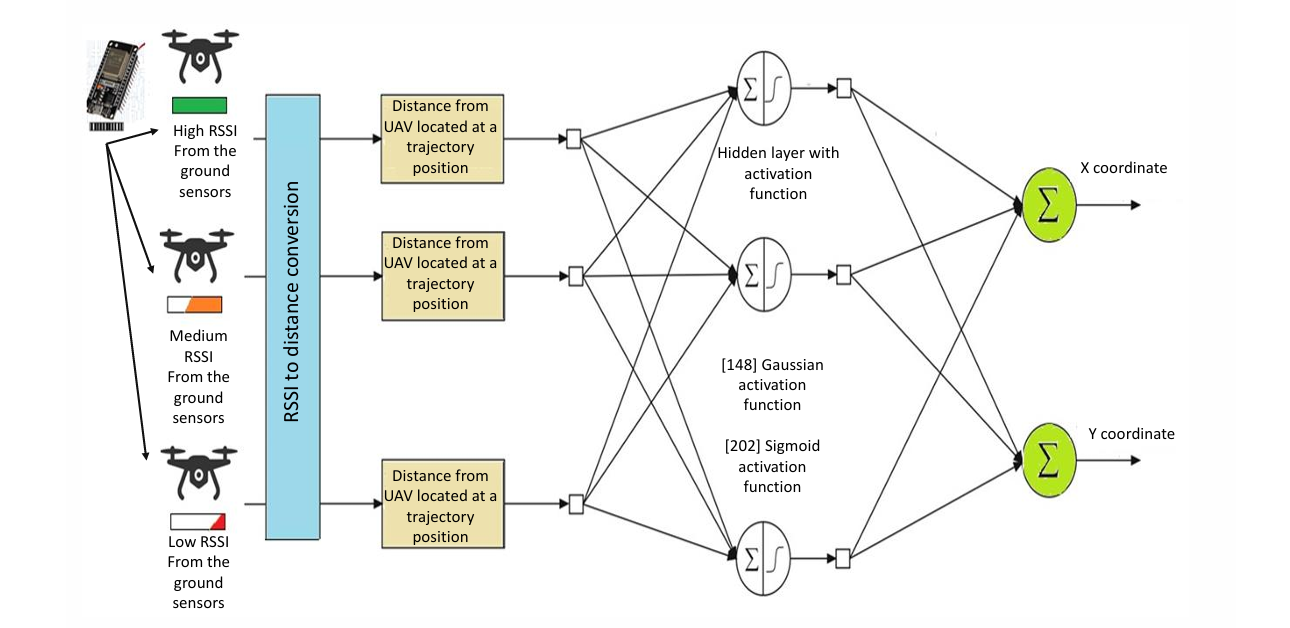
\includegraphics[width=0.7\textwidth]{Figures/Chapter2/Section1/1.png}
\caption{The MLP for UAV-based localization of a WSN node using the Gaussian activation function \cite{annepu2020uav} and the RBF model
 using the Sigmoid activation function \cite{annepu2021radial}}
\label{fig:mlp-uav-localization}
\end{figure}


In UAV-aided image analysis, challenges like camera pose variations, shadows, and illumination changes often stem from noise or acquisition issues. Autoencoders address these by clustering image features based on similarity, with the encoder network learning to distinguish dynamic changes through training and reduces the required number of training images.




%%%%%%%%%%%%%%%%%%%%%%%%%%%%%%%%%%%%%%%%%%%%%%%%%%%%%%%%%%%%%%%%%%%%%%

\subsubsection{ Semi-supervised Learning for UAV Trajectory Opti
mization}



A Generative Adversarial LSTM (GA-LSTM) network can be used to optimize resource allocation in UAV-assisted machine-to-machine wireless communications. This architecture combines the capabilities of Generative Adversarial Networks (GANs) and Long Short-Term Memory (LSTM) networks to jointly optimize transmit power, communication mode, frequency channel selection, and UAV selection and trajectory within a partially observable multi-agent environment. The LSTM component enables the tracking of UAV movements and supports reward evaluation. Numerical evaluations show that this integrated model achieves higher sum rates compared to standalone LSTM or Deep Q-Network (DQN) methods.

In cellular networks that include both UAV-based aerial base stations (BSs) and ground BSs, a Gaussian Mixture Model (GMM) with weighted expectation-maximization can be employed to represent the spatial traffic distribution and guide base station deployment, including UAV positioning. This technique allows for traffic congestion prediction and determines the optimal placement of UAVs to reduce energy costs related to both communication and relocation. Simulation results highlight energy savings of up to 20\% for communication and 80\% for relocation when compared to heuristic approaches.




%%%%%%%%%%%%%%%%%%%%%%%%%%%%%%%%%%%%%%%%%%%%%%%%%%%%%%%%%%%%%%%%%%%%%%

\subsubsection{Reinforcement Learning for Joint Trajectory Plan
ning and Mission Scheduling}


Deep Reinforcement Learning (DRL) techniques offer innovative approaches for planning UAV trajectories in dynamic environments.


\paragraph{Deep Q-Network with Trajectory Discretization}




In UAV-assisted communications, reinforcement learning approaches like Q-learning face challenges with large state/action spaces, prompting the use of Deep Q-Networks (DQNs) which leverage neural networks to handle extended spaces. DQNs have been particularly effective for Age of Information optimization, where they balance energy efficiency with data freshness while using autoencoders with LSTM to manage large state spaces through spatiotemporal feature extraction ~\cite{abedin2020data,ferdowsi2021neural}.


\begin{figure}[H]
\centering
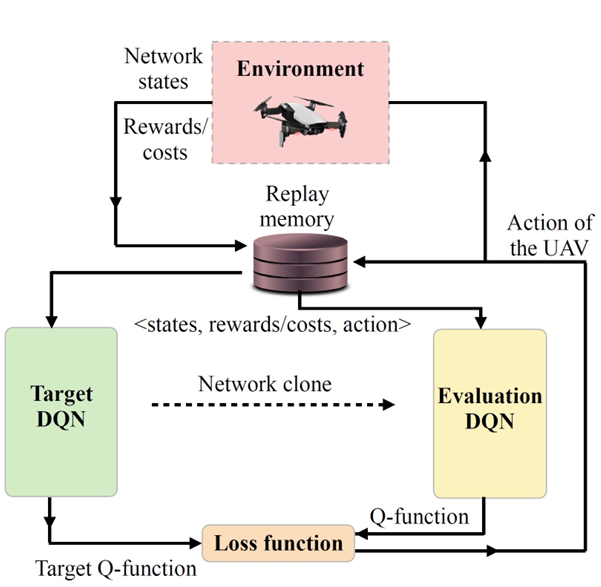
\includegraphics[width=0.7\textwidth]{Figures/Chapter2/Section1/2.png}
\caption{ Schematic overview of a DQN-based framework for UAV trajectory and mission planning. The model is deployed onboard the UAV and trained to generate optimal policies for both path planning and radio resource allocation. \cite{kurunathan2022machine}}
\label{fig:dqn_trajectory_planning}
\end{figure}



For throughput and energy optimization, deep Q-networks (DQNs) are used to jointly optimize UAV trajectories and bandwidth allocation. These methods take into account node states and data volume to enhance overall network performance. Packet loss issues are mitigated by adjusting UAV velocity and scheduling communications based on real-time data, including battery levels, queue statuses, and channel conditions.

In coverage-oriented applications, DQNs are applied to maintain robust network connectivity. They dynamically adapt to changes in topology and optimize UAV paths to balance coverage fairness and energy consumption. Advanced versions such as dueling DQNs are employed for scenarios requiring optimized flight paths for uplink throughput. These approaches also integrate obstacle avoidance and prioritize data with latency sensitivity.

In UAV-assisted Mobile Edge Computing (MEC) systems, double DQNs support effective task offloading decisions. This improves throughput while managing energy limitations and addressing data security challenges like eavesdropping. Wireless power transfer systems benefit from DQN-based optimization techniques as well, especially for planning UAV trajectories and selecting energy-harvesting nodes. These strategies are sometimes enhanced using probabilistic algorithms such as Naive Bayes for estimating node locations.

Although these techniques have broad applicability, their reliance on discrete action spaces poses a limitation. This constraint reduces their suitability for continuous control problems, such as fine-tuned UAV cruise control, highlighting the need for alternative or hybrid approaches in such contexts.




%%%%%%%%%%%%%%%%%%%%%%%%%%%%%%%%%%%%%%%%%%%%%%%%%%%%%%%%%%%5

\paragraph{Online Trajectory Planning With Deep Deterministic
 Policy Gradient}



The Deep Deterministic Policy Gradient (DDPG) algorithm effectively combines value iteration and policy iteration approaches, offering a robust framework for deep reinforcement learning in continuous state and action spaces. Unlike Deep Q-Networks (DQN), which predict Q-values for discrete state-action pairs, DDPG employs a dual-network structure: a critic network that estimates Q-values and an actor network that determines optimal actions. This architecture allows DDPG to manage continuous control problems more efficiently than traditional DQN methods.

\begin{enumerate}

\item \textbf{Cruise Control:} DDPG demonstrates strong capabilities in UAV cruise control by learning optimal headings and velocities to minimize network costs in continuous action spaces. Its experience replay mechanism improves training stability by reusing past learning samples. Applications include autonomous landing on dynamic platforms, air combat maneuvering through precise trajectory control, and urban navigation that integrates obstacle avoidance with energy-efficient route planning.

\item \textbf{Age of Information (AoI):} DDPG is effective in minimizing the Age of Information by adapting to dynamic traffic and environmental conditions. Advanced variants like twin delayed DDPG (TD3) improve energy efficiency while maintaining low AoI in IoT networks. Multi-agent extensions enhance trajectory learning, and policy-based enhancements enable optimization of flight altitude and transmission scheduling.

\item \textbf{UAV-assisted MEC:} In Mobile Edge Computing scenarios, DDPG handles complex action spaces, making it suitable for joint optimization of content caching, delivery, and power control. It plays a key role in vehicular networks, managing spectrum and computing resource allocation and addressing the multifaceted challenges of UAV-assisted MEC environments.

\item \textbf{Other Applications:}
\begin{itemize}
    \item Deep reinforcement learning-based frameworks have achieved improved fairness and energy efficiency in coverage and resource allocation.
    \item Game-theoretic approaches combined with DDPG enable optimal UAV deployment and trajectory planning while ensuring obstacle avoidance.
    \item Hybrid systems integrating DDPG with LSTM networks facilitate dynamic spectrum sharing through intelligent timeslot allocation.
    \item Enhanced Q-network variants have been applied to outage minimization and integrated navigation with radio environment mapping.
\end{itemize}

\end{enumerate}





\begin{figure}[ht]
\centering
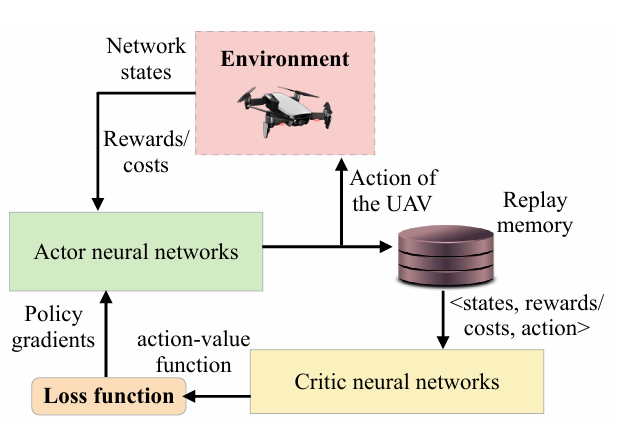
\includegraphics[width=0.7\textwidth]{Figures/Chapter2/Section1/4.png}
\caption{DDPG Architecture Overview with Actor-Critic Networks and Experience Replay for UAV Control \cite{kurunathan2022machine}}
\label{fig:ddpg_uav_control}
\end{figure}


%%%%%%%%%%%%%%%%%%%%%%%%%%%%%%%%%%%%%%%%%%%%%%%%%%%%%%%%%%%

\paragraph{Multi-agent DRL for Multi-UAV Cooperation}

The multi-agent DQN framework has been successfully implemented for cooperative UAV systems, where the network state incorporates ground nodes' battery levels, data queue statuses, and all UAV waypoints~\cite{dqn_multi_115}. This approach enables intelligent scheduling of ground node transmissions while dynamically adapting to changing data and energy arrival patterns.

Building upon this foundation, researchers have enhanced the multi-agent DQN framework to incorporate velocity adjustment capabilities at waypoints, while maintaining optimal ground node selection for data transmission. This extension provides more refined control over UAV movements during mission execution.

For cellular network applications, multi-agent DQN can effectively address the complex joint optimization of UAV trajectories and communication scheduling. The solution coordinates data transmissions from cellular tower ground nodes based on relative positions between UAVs and ground stations.

In energy conservation scenarios, a non-cooperative game formulation with periodic UAV beaconing establishes optimal beaconing equilibrium durations without requiring knowledge of other UAVs' transmission schedules.

Security applications have leveraged multi-agent DDPG approaches, where UAV jammers are coordinated to enhance secure channel capacity. The framework simultaneously optimizes jammer trajectories, jamming power levels, and legitimate UAV transmission power.

For MEC systems, a multi-agent DDPG model improves resource allocation fairness while optimizing UAV trajectories and computation offloading decisions to boost MEC device energy efficiency.

Further advancing MEC applications, a comprehensive multi-agent DDPG framework for vehicular networks treats the MEC server as an intelligent agent coordinating UAV and ground vehicle scheduling, along with computational resource allocation. Integration with federated learning significantly improves task offloading performance from vehicles to UAVs.

\begin{figure}[h!]
\centering
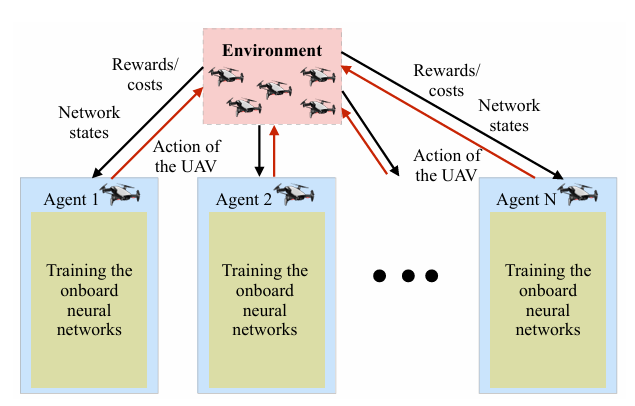
\includegraphics[width=0.8\textwidth]{Figures/Chapter2/Section1/5.png}
\caption{A multi-agent DRL structure where each UAV trains an onboard neural network to determine the optimal joint actions~\cite{kurunathan2022machine}}
\label{multi_agent_drl_structure}
\end{figure}

\textbf{Note:} The selection between multi-agent DQN and DDPG implementations depends on the action space characteristics of the target application. DQN is preferred for discrete decision spaces (e.g., UAV clustering), while DDPG excels in continuous control scenarios (e.g., precise trajectory planning). Complementary techniques like autoencoding further enhance these frameworks through efficient feature extraction and supervised learning components.







%%%%%%%%%%%%%%%%%%%%%%%%%%%%%%%%%%%%%%%%%%%%%%%%%%%%%%%%%%%%%%%%%%%%%%

\subsection{Machine Learning for UAV Perception and Feature Extraction}


Feature extraction is a technique for reducing dimensionality. It typically begins with a set of real-time data collected through the UAV's camera, followed by the creation of derived values (such as edges, shapes, and object recognition) that carry meaningful information. This derived learning is non-redundant and supports subsequent learning to enhance feature extraction. Unlike traditional imaging platforms, UAVs offer a unique vantage point, providing an expansive view of the area of interest. Additionally, the mobility of UAVs allows them to cover a larger geographical area compared to stationary imaging systems. In the following sections, we explore key machine learning techniques applied to UAV-assisted imaging.


\subsubsection{Supervised Learning-based UAV Operations}



Supervised machine learning techniques, like MLP, are capable of processing information through multiple layers, assisting in the interpretation of images captured by the UAV. Approaches such as CNN can segment and link the layers of an image, facilitating feature extraction.

\begin{enumerate}
    \item \textbf{Multilayer Perceptron for Image Processing}

    UAVs have gained significant traction in precision agriculture, particularly in crop disease analysis and vegetation management, where MLP models demonstrate notable effectiveness. In \cite{Abdulridha2020}, a UAV equipped with hyperspectral cameras captures hyperspectral images of a tomato field to facilitate early disease detection caused by fungus and bacteria. An MLP neural network classifies the images, achieving an impressive accuracy rate of 99\%. In an other approach a quadcopter UAV, outfitted with a Raspberry Pi single-board computer and an onboard camera module, is employed for vegetation mapping in tomato crops. MLP is used to segment the crop images, outperforming the support vector machine (SVM) alternative in terms of precision and recall.

    The utility of MLP in aerial image analysis extends beyond agriculture to environmental management, such as weed eradication \cite{Tamouridou2017}. In this study, a multi-spectral camera is mounted on an eBee fixed-wing UAV to capture high-resolution images of a field. An MLP with automatic relevance detection (MLP-ARD) is used to detect the weed species *Silybum marianum* among various types of vegetation. The MLP, featuring one hidden layer and one output unit, is regulated through Bayesian regularization to prevent overfitting and is trained on spectral and textural input data to classify the weed effectively. MLP has also been applied to flood management, with UAVs capturing aerial images of flooded areas in Houston, Texas. In this case, an MLP is used for semantic analysis following the use of a densely connected CNN and RNN to process the images.
    
    Furthermore, MLP models have proven useful in UAV route planning and agricultural harvesting. In \cite{annepu2020uav}, UAVs assist in route planning and harvest volume estimation for unmanned agricultural harvesting systems, addressing the challenge of harvest losses due to untimely collection. The UAV, equipped with multi-spectral cameras, captures images that are analyzed using various neural networks, including MLP. The MLP, with three neurons in the hidden layer, provides optimal performance compared to other tested models, such as generalized regression networks and radial basis function networks.
    

    
    \item \textbf{Convolutional Neural Network for Image Processing}

    CNN is widely utilized for classifying and segmenting remotely sensed imagery due to its ability to extract detailed features. In UAV forest imagery, CNN can effectively identify features such as vegetation and dry areas. It is also employed in multi-object tracking for real-time applications, where it associates objects efficiently. Challenges arise from poor radio connections between the UAV and the base, which can degrade the quality of transmitted images, leading to packet loss and bandwidth wastage. A solution for this issue involves an Optimal Strategy Library (OSL) for video encoding, which adapts to the packet loss rate and bandwidth, ensuring improved video sequence encoding and recovery of partially corrupted videos \cite{kurunathan2022machine}.
    
    CNN-based approaches have shown high precision and accuracy (around 90\%) in detecting slope failures from UAV remote sensing imagery. Similar performance is observed in several other image classification applications, where CNN achieves over 90\% accuracy. In high-throughput phenotyping using high-resolution multispectral imaging, CNN classification and segmentation techniques provide nearly 99\% accuracy. For search and rescue operations, UAVs with video cameras can analyze avalanche debris, and CNN can identify features indicative of survivors. Additionally, a linear Support Vector Machine (SVM) can be used in conjunction with CNN to enhance object detection.
    
    CNN excels in imaging applications such as localization, object detection, and segmentation. Despite its strengths, one limitation is the time, energy, and resources required for segmentation tasks. To address this, techniques like recurrent CNN (R-CNN) have been developed to streamline the processing. In certain UAV imagery applications, R-CNN improves detection accuracy and resolves issues related to image resolution. Lightweight CNN architectures have also been proposed for efficient execution on embedded processors, providing a balance between performance and resource consumption. Energy-aware designs have been suggested to minimize power consumption in UAV tracking and landing tasks, with CNN's Quality of Service (QoS) level adjusting to save energy.
    
    Although CNN is highly effective, it does not encode object position and orientation, and its detailed segmentation process can be resource-intensive. The layers closer to the CNN input focus on simple features such as edges, corners, and endpoints, but deeper layers, which offer more complex feature extraction, require longer training times. To mitigate this, lightweight CNN models have been introduced to reduce the need for powerful GPUs. Additionally, integrating Recurrent Neural Networks (RNN) with CNNs has shown promise in improving image processing, where dense connections enhance information flow and gradient propagation, thus improving training efficiency and reducing overfitting. This integration has achieved impressive results, with reported accuracy rates of 96\% on real-world datasets.
    

    \begin{figure}[H]
        \centering
        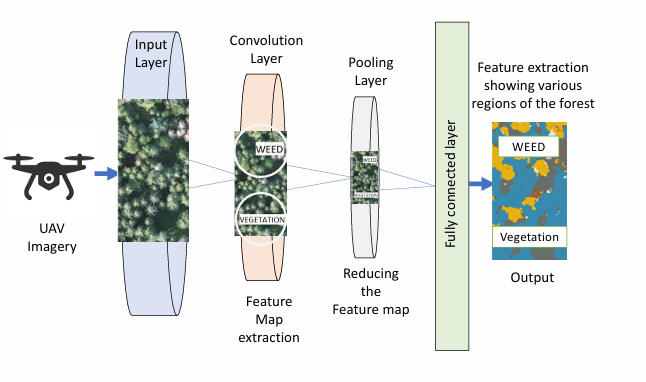
\includegraphics[width=0.7\textwidth]{Figures/Chapter2/Section1/6.png}
        \caption{Convolutional Neural Networks in Image Processing~\cite{kurunathan2022machine}}
        \label{cnn_image_processing}
    \end{figure}

\end{enumerate}



\subsubsection{Unsupervised Learning-based Approaches}
    
    Novel unsupervised learning techniques, such as spiking neural networks (SNN), have energy-efficient and high-processing capabilities, making them suitable for faster and more energy-efficient control decisions in UAV operations. Neuromorphic SNNs utilize temporal difference learning to predict both rewards and temporal sequences in physical time. Temporal difference learning can be achieved by analyzing the temporal distance between neighboring events that vary in decay time constant. Neuromorphic SNNs replicate the functionality of a central nervous system, and typically operate at orders of magnitude lower power than traditional computing systems. This low-power capability is due to the event-driven, massively parallel nature of SNNs, where only a small portion of the system is active at any given time while the rest remains idle. This makes them suitable for applications such as edge computing, where strict energy constraints exist \cite{kurunathan2022machine}. 


    \begin{figure}[H]
        \centering
        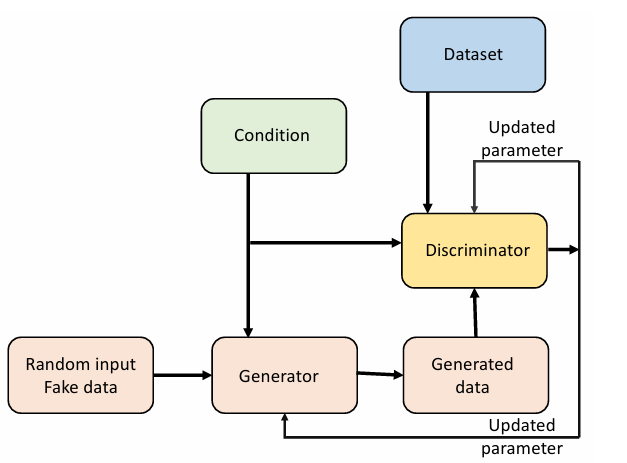
\includegraphics[width=0.7\textwidth]{Figures/Chapter2/Section1/7.png}
        \caption{Generative Adversarial Network Framework for UAVs~\cite{kurunathan2022machine}}
        \label{GAN_UAV}
    \end{figure}
    To leverage the ultra-low-power capabilities of neuromorphic processors (on the order of several milliwatts), a neuromorphic SNN model has been studied for onboard deployment in UAVs to control their movements for obstacle avoidance. Differential evolution and Bayesian optimization are used to obtain the optimal configuration for the SNN. An SNN-based proportional-integral-derivative (PID) controller has been integrated with UAV motor control to ensure ultra-low power consumption while maintaining a high processing rate. In this architecture, each spiking neuron carries sensor measurements and control information, firing a spike when thresholds or biases are reached.
    
    SNNs are also studied to control a hexacopter UAV in six degrees of freedom: yaw, roll, pitch, height, position, and angular velocity. A recurrent spiking controller is proposed to solve nonlinear control problems in continuous domains using a topology evolution algorithm as the learning mechanism. The results suggest that SNNs can solve ongoing control problems by maintaining sufficient spike activities and decoding from weighted spike frequencies. Additionally, an unsupervised Spike Time Dependent Plasticity (STDP) approach has been developed to detect UAVs in images. This asynchronous system, utilizing event-based camera features, is both low in power consumption and computational overhead.
    
    A decision-making model for UAV flight control uses an SNN to simulate brain zone functions, determining control actions based on the relative positions of obstacles and the UAV. A system has been developed where spiking neurons detect and locate obstacles by partitioning the onboard camera image and mapping it for navigation. One SNN model, the liquid state machine, can track network states over time and predict data feature distributions. Liquid state machines have also been applied to resource allocation in cache-enabled UAVs, learning the data request distribution from ground nodes and determining data caching policies for the UAV.
    
    % \textbf{Remark:} Due to their ability to process data recurrently and constantly learn from the environment, methods like RNNs are well-suited for UAV control. Techniques like SNNs bring the advantage of energy efficiency to UAV operations. Machine learning (ML) methods are also used for real-time waypoint setting and smart trajectory planning for applications such as data collection and sensing.
    
    
%%%%%%%%%%%%%%%%%%%%%%%%%%%%%%%%%%%%%%%%%%%%%%%%%%%%%%%%%%%%%%%%%%%%%%

\subsection{Machine Learning for Feature Interpretation and Regeneration}


Feature extraction is a form of dimensionality reduction. Feature extraction, pattern recognition, and image processing usually start from an actual set of measured data (taken through the camera of the UAV). It builds derived values (features such as edges, shapes, object recognition) that are informative. This derived learning is non-redundant and facilitates subsequent learning to obtain better feature extraction. UAVs can provide an eagle-eyed view of the region of interest compared to their counterparts, i.e., the non-UAV imaging platforms. The mobility of UAVs can also provide the capability to cover a larger geographical area than their stationary counterparts \cite{244}. In what follows, we discuss important ML techniques used in UAV-assisted imaging.


\subsubsection{Feature interpretation by Linear Regression}



The use of UAVs for environmental observation and agricultural monitoring has been growing steadily. These aerial platforms collect various types of sensory data through onboard instruments like cameras and infrared sensors. One of the most widely adopted techniques for analyzing such data is linear regression (LR), along with its different extensions.

Linear regression, a core technique in supervised machine learning, is employed to model the relationship between a set of input features and a continuous target output. This approach provides numerical insight into how features influence the target variable, offering a way to explain and quantify feature importance.

In one application, LR was used to evaluate how the spatial placement of sensors affects air pollution measurements in a UAV-based system \cite{villa2016uav}. This study also proposed design guidelines for UAV systems tasked with locating emission sources.

In the field of precision agriculture, LR helped establish a correlation between the crop coefficient and the normalized difference vegetation index to estimate evapotranspiration \cite{niu2020estimating}. A deep stochastic configuration network was also utilized to complement the LR model and enhance predictive performance.

Other research combined plant height and vegetation indices derived from UAV imagery to estimate biomass using a multiple LR model. Additionally, structure-from-motion (SfM) techniques were applied to generate 3D point clouds from overlapping aerial images. These were used to evaluate the health of wetland vegetation by linking them to vegetation indices through LR models.

In bathymetric mapping, LR’s limitations were addressed by introducing a geographically weighted regression (GWR) model, which improved accuracy and reduced the spatial biases often present in standard multiple regression approaches .

For soil salinity mapping, advanced regression techniques such as random forest models were applied on data collected from electromagnetic induction sensors and hyperspectral cameras.

Although LR is easy to implement and interpret, it assumes a linear relationship between inputs and outputs. This assumption can lead to poor model performance when the actual relationship is more complex. Furthermore, LR is sensitive to noise and prone to overfitting, especially when the number of input features exceeds the number of available observations.



\subsubsection{Classification by K-Means Clustering}

K-means clustering has been effectively applied in path planning for multi-UAV systems, particularly when coordinating multiple tasks within a designated area. Given the geographic distribution of tasks, K-means is used to group them into several clusters. Each cluster can then be assigned to a UAV, and route optimization techniques—such as simulated annealing or genetic algorithms—are employed to determine efficient paths within those clusters.

In addition to task allocation, K-means plays a role in guiding UAV movement for coverage-related objectives. For instance, in scenarios where UAVs are deployed to deliver cellular connectivity, the approach dynamically groups users based on their spatial positions. UAVs are then directed to the centroids of these groups to ensure adequate coverage and maintain service quality. This method has demonstrated convergence toward locally optimal deployments. Similar strategies have also been implemented in aerial surveillance tasks to ensure efficient area monitoring using multiple UAVs.







    \begin{figure}[H]
        \centering
        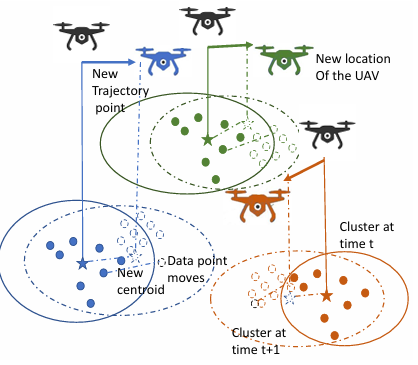
\includegraphics[width=0.7\textwidth]{Figures/Chapter2/Section1/8.png}
        \caption{Centroid-Based Coordination in Multi-UAV Surveillance Using K-Means Clustering~\cite{huang2021navigating}}
        \label{centroid_kmeans_uav}
    \end{figure}








\subsubsection{Environment Modeling Using Gaussian Mixture Models}


GMM (Gaussian Mixture Model) is applied to model static, complex-shaped, two-dimensional obstacles, aiding in the prevention of UAV collisions. Given prior probabilistic knowledge about obstacles, GMM is generated to form the potential field of the target area. The parameters of the GMM are iteratively estimated using the Expectation-Maximization (EM) method, allowing the model to approach the true distribution of the obstacles. By taking derivatives over the GMM, the potential field is created, and UAV flight paths are determined by following the field directions. A trajectory prediction model based on GMM clusters trajectory data into distinct components and applies Gaussian process regression to predict possible future trajectories. Additionally, GMM is utilized to create heatmaps of object detection probabilities in a designated area. For instance, a UAV can be used to maximize the probability of locating a specific object by planning an efficient flight path, taking into account environmental factors like foliage coverage, shadowing, and illumination. The spatial distribution of detection probabilities is modeled using GMM, which aids in creating a hierarchical search plan for a mission. 


    \begin{figure}[H]
        \centering
        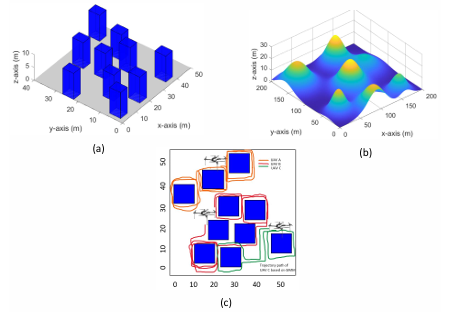
\includegraphics[width=0.7\textwidth]{Figures/Chapter2/Section1/9.png}
        \caption{Trajectory Planning for UAVs Using GMM-Based Environment Modeling~\cite{huang2021navigating}}
        \label{trajectory-planning-gmm}
    \end{figure}





Furthermore, GMM is integrated with horizon control techniques to optimize the trajectories of multiple UAVs tasked with searching a complex environment. In these setups, receding horizon control (model predictive control, MPC) is used for dynamic path planning to optimize search efforts, avoid collisions, and ensure simultaneous arrival at a target. Cooperation among UAVs is facilitated by regular flight path broadcast messages. GMM is also used to model the distribution of radio traffic in cellular networks involving UAV-based base stations (BSs), which helps in optimizing UAV placement. By utilizing a weighted EM algorithm, GMM can predict traffic congestion and reduce UAVs' energy consumption for communication and mobility. Simulations indicate a reduction of 20\% in communication energy use and 80\% in mobility energy compared to heuristic methods.

In conclusion, techniques such as K-means clustering and linear regression are effective in feature interpretation and environmental data analysis, while probabilistic models like GMM excel at spatial distribution modeling and feature classification. These methods prove highly accurate when sufficient prior data is available, enabling complex applications like UAV control.




%%%%%%%%%%%%%%%%%%%%%%%%%%%%%%%%%%%%%%%%%%%%%%%%%%%%%%%%%%%%%%%%%%%%%%
%%%%%%%%%%%%%%%%%%%%%%%%%%%%%%%%%%%%%%%%%%%%%%%%%%%%%%%%%%%%%%%%%%%%%%
%%%%%%%%%%%%%%%%%%%%%%%%%%%%%%%%%%%%%%%%%%%%%%%%%%%%%%%%%%%%%%%%%%%%%%

\section{Security in UAVs networks}


\subsection{taxonomy of security threats based on threat vectors}

    This section introduces a structured overview of security threats in FANETs, organized according to threat vectors, as depicted in Figure~\ref{fig:FANET_threats}. These vectors include six types of connections and six distinct node categories. A total of 20 threats are analyzed and categorized based on both their impact on security requirements and their relevance to different network architectures.
    
    Utilizing the STRIDE threat modeling framework, we identify specific vulnerabilities affecting both node and connection layers (see Figure~\ref{fig:FANET_threats}). 
    
    Out of the 20 threats, 15 pertain to connection-level vulnerabilities, while the remaining five are associated with node-level issues. To address these threats, 15 mitigation strategies have been proposed. These strategies span six types of networks: 5G mobile networks, FANETs, general Ad-Hoc networks, RW, WLAN, and WSN.
    
    


    \begin{figure}[H]
        \centering
        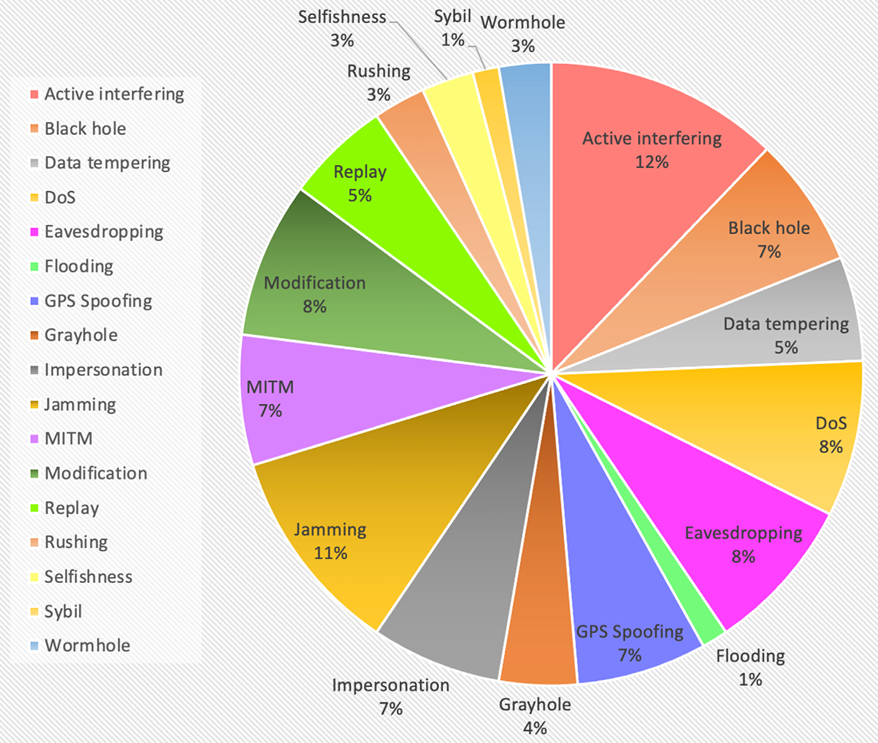
\includegraphics[width=0.7\textwidth]{Figures/Chapter2/Section2/1.png}
        \caption{Percentage of security threats in FANETs~\cite{tsao2022survey}}
        \label{fig:FANET_threats}
    \end{figure}
    

\subsubsection{Threat vectors}








The following section analyzes the primary security threats that can affect each communication link within a typical UAV ground and aerial system. These links—ranging from user interfaces to inter-UAV communication—are potential vectors for attacks targeting confidentiality, integrity, availability, or authenticity. For each connection, we identify common threats and describe them succinctly for clarity and reference.

\paragraph{C1: Client terminal to GCS.}

This connection involves the user interface where operators input commands or receive feedback. It is vulnerable to insider misuse, eavesdropping, and message replay.

\begin{itemize}
    \item \textbf{Eavesdropping:} Interception of sensitive data such as commands or credentials, which compromises confidentiality.
    \item \textbf{Insider threat:} Authorized users misusing their access to compromise the system's integrity.
    \item \textbf{Replay attack:} Reuse of captured messages to produce misleading outcomes, affecting authenticity.
\end{itemize}

\paragraph{C2: GCS to Backbone UAV.}

This link is critical for command and control and is transmitted via wireless media that differ in vulnerability. The security depends heavily on the medium used.

\begin{table}[H]
\renewcommand{\arraystretch}{1.3}
\centering
\caption{Transmission medium vulnerabilities for C2.}
\begin{tabular}{|>{\centering\arraybackslash}m{3.5cm}|
                >{\centering\arraybackslash}m{2.5cm}|
                >{\arraybackslash}m{7.5cm}|}
\hline
\textbf{Medium} & \textbf{Security Level} & \textbf{Vulnerabilities} \\
\hline
WiFi & Medium & Susceptible to interception if not strongly encrypted; can be mitigated using non-standard frequency bands. \\
\hline
RF & Low & Sensitive to interference; careful channel selection and control are needed. \\
\hline
Satellite & High & Generally more secure but expensive and less commonly used in civilian operations. \\
\hline
\end{tabular}
\label{tab:c2_mediums}
\end{table}

\vspace{1em}

The communication from GCS to UAVs is open to several attacks, particularly due to wireless exposure. The table below details key threats targeting this path.

\begin{table}[H]
\renewcommand{\arraystretch}{1.3}
\centering
\caption{Threats on the GCS–Backbone UAV connection (C2).}
\begin{tabular}{|>{\centering\arraybackslash}m{3.5cm}|
                >{\centering\arraybackslash}m{2.5cm}|
                >{\arraybackslash}m{7.5cm}|}
\hline
\textbf{Threat} & \textbf{Category} & \textbf{Description} \\
\hline
Eavesdropping & Confidentiality & Leakage of mission-critical information or positioning data. \\
\hline
Jamming & Availability & Intentional or accidental signal disruption, breaking communication. \\
\hline
Man-in-the-middle & Integrity & Interception and manipulation of exchanged messages. \\
\hline
Replay attack & Authenticity & Reusing valid packets to disrupt or trick the communication logic. \\
\hline
\end{tabular}
\label{tab:c2_threats}
\end{table}

\paragraph{C3 and C4: Backbone UAV to other UAVs.}

These connections support swarm behavior and inter-UAV coordination. Their wireless nature makes them highly sensitive to disruptions and impersonation threats.

\begin{table}[H]
\renewcommand{\arraystretch}{1.3}
\centering
\caption{Threats on Backbone-to-UAV and inter-UAV connections (C3, C4).}
\begin{tabular}{|>{\centering\arraybackslash}m{3.5cm}|
                >{\centering\arraybackslash}m{2.5cm}|
                >{\arraybackslash}m{7.5cm}|}
\hline
\textbf{Threat} & \textbf{Category} & \textbf{Description} \\
\hline
Eavesdropping & Confidentiality & Unauthorized interception of UAV status or swarm coordination commands. \\
\hline
Jamming & Availability & Signal blocking that affects the swarm’s ability to coordinate. \\
\hline
Man-in-the-middle & Integrity & Rogue UAVs impersonate legitimate ones to alter, delay, or block communication. \\
\hline
Replay attack & Authenticity & Repetition of past messages to cause confusion or misalignment in swarm behavior. \\
\hline
\end{tabular}
\label{tab:c3_c4_threats}
\end{table}






\subsubsection{Security threats on nodes}

Security threats on nodes, including client terminals, GCS, and UAVs, can disrupt FANET operations. If a node fails to forward messages, another node may take control of the mission.

\textbf{Client terminal.} Client terminals can be attacked to send malicious or fake commands, depending on their hardware and operating systems.

\textbf{GCS and backbone UAV, single point of failure (SPOF).} The reliance on a single GCS and backbone UAV is a vulnerability. Implementing multiple GCSs and UAVs enhances resilience by ensuring automatic operation in case of failure.

\textbf{UAVs.} UAVs face several major threats:

\begin{itemize}
    \item \textbf{Backdoor.} UAVs can contain backdoors that allow external control, hijacking their operation. ~\ref{fig:Maldrone_Attack} shows a Maldrone attack.

    \begin{figure}[H]
        \centering
        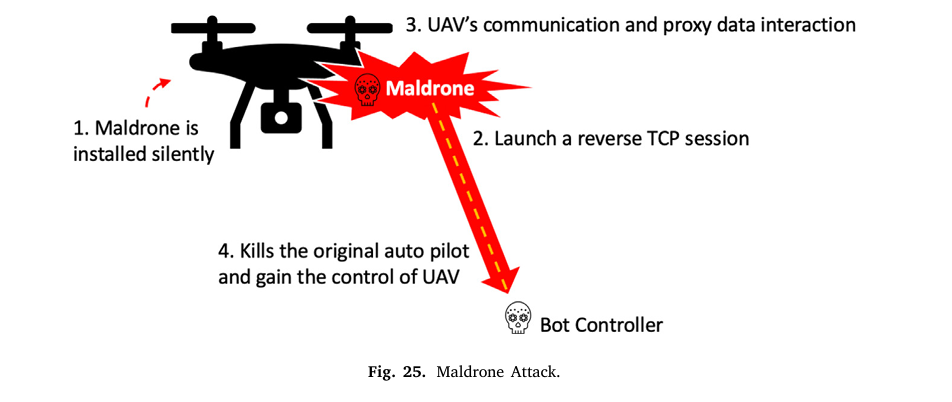
\includegraphics[width=0.7\textwidth]{Figures/Chapter2/Section2/4.png}
        \caption{ Maldrone Attack ~\cite{tsao2022survey}}
        \label{fig:Maldrone_Attack}
    \end{figure}
    
    \item \textbf{Denial of Service (DoS) attack.} Attackers can overload UAVs with fake messages, preventing new missions or disrupting flight paths. ~\ref{fig:DoS_Attack} shows a DoS attack on UAV 1.

    \begin{figure}[H]
        \centering
        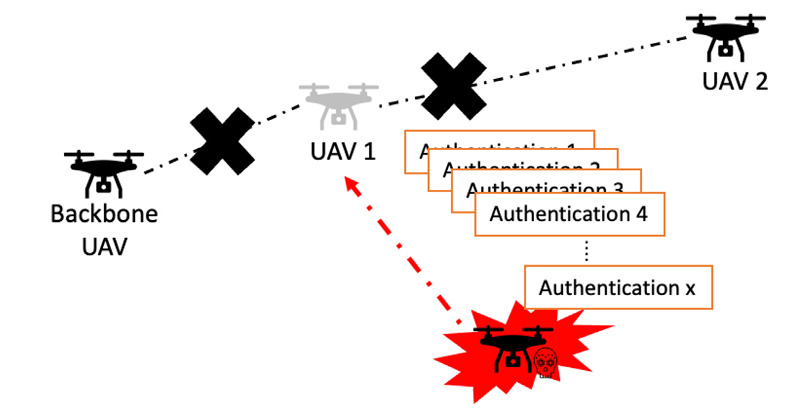
\includegraphics[width=0.7\textwidth]{Figures/Chapter2/Section2/5.png}
        \caption{  DoS Attack ~\cite{tsao2022survey}}
        \label{fig: DoS_Attack}
    \end{figure}
    
    \item \textbf{Flooding attack.} Sending large volumes of data to UAVs can deplete their resources, causing malfunctions.
    
    \item \textbf{Selfishness/selfish node.} UAVs low on energy may reduce performance by failing to forward data to others, degrading network efficiency. ~\ref{fig:IOD_system} shows an example of a selfish node

    \begin{figure}[H]
        \centering
        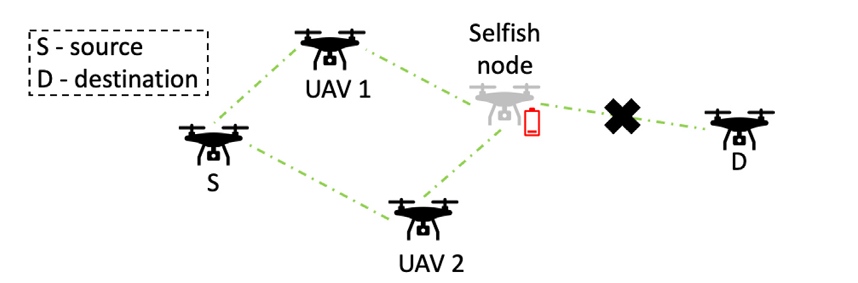
\includegraphics[width=0.7\textwidth]{Figures/Chapter2/Section2/6.png}
        \caption{  Selfish Node ~\cite{tsao2022survey}}
        \label{fig: Selfish_Node}
    \end{figure}
    
    \item \textbf{Cloud server and storage, data tampering.} Modifying stored data in cloud databases can compromise privacy or disrupt operations.
\end{itemize}



\subsubsection{Security threats on the IoD}

The Internet of Drones (IoD) faces several security and privacy challenges. Drones often lack built-in protections, making them prone to data leaks and attacks. Hardware constraints lead to reliance on lightweight encryption and processing protocols. Airspace is divided into zones connected by gates, with each zone having mapped routes and intersections. Zone Service Providers (ZSPs) deliver navigational data to assist drone operations. Figure~\ref{fig:IOD_system} illustrates the overall structure of the IoD communication system.


\subsubsection{Confidentiality}
IoD systems handle sensitive data such as locations, flight paths, and drone identities, which could be exploited for physical attacks. Systems must support drone identification when needed, while minimizing exposure. Insider threats, including personnel with privileged access, can pose significant risks.

\subsubsection{Integrity}
Limited processing power in drones and ZSPs leads to offloading tasks to cloud services. Unencrypted data is vulnerable to unauthorized access. Large datasets like video streams may be difficult to encrypt, and even when encrypted, processing limitations hinder efficient indexing and search.

\subsubsection{Availability}
ZSP-drones communication links are attractive targets for denial-of-service, spoofing, and data injection attacks. These threats may require external auditing to detect. Trusted computing platforms can help enforce system integrity, though they may introduce latency or false alarms.

    \begin{figure}[H]
        \centering
        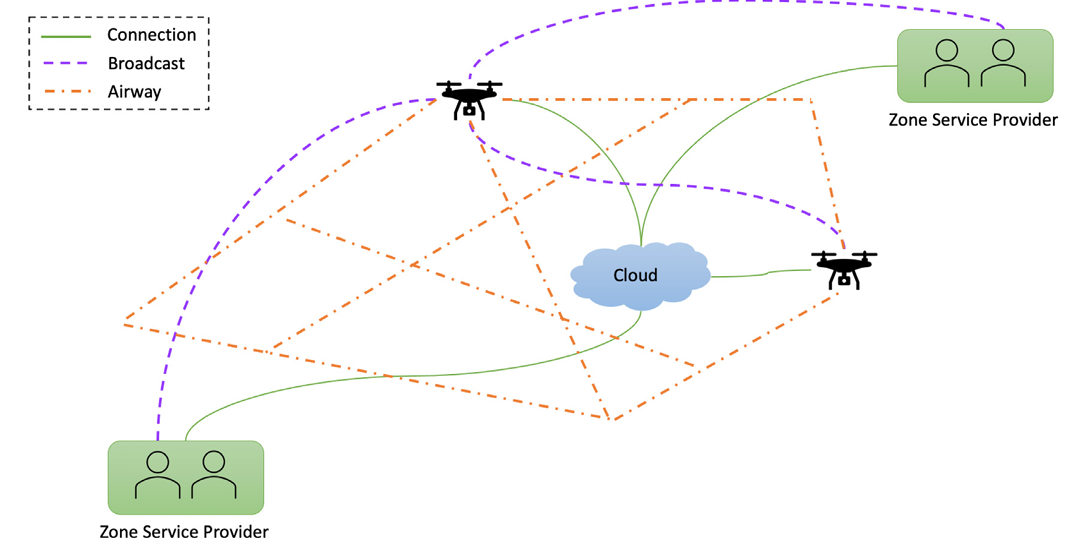
\includegraphics[width=0.7\textwidth]{Figures/Chapter2/Section2/3.png}
        \caption{ IoD Communication System Overview ~\cite{tsao2022survey}}
        \label{fig:IOD_system}
    \end{figure}

%%%%%%%%%%%%%%%%%%%%%%%%%%%%%%%%%%%%%%%%%%%%%%%%%%%%%%%%%%%%%%%%%%%%%%
\section{Security solutions and standards}

As UAVs in Flying Ad-Hoc Networks (FANETs) become more prevalent, securing their communication and operations against various threats is essential. These threats include jamming, malware, data tampering, and blackhole attacks, among others. This section examines the key security challenges in FANETs and outlines the solutions developed to address them. These solutions vary from agent-based approaches, which rely on UAV-specific agents, to agent-less methods, depending on the resources available. The section also covers essential security requirements, such as availability, confidentiality, and integrity, which are critical to ensuring the secure operation of UAV networks.

    \begin{figure}[ht]
        \centering
        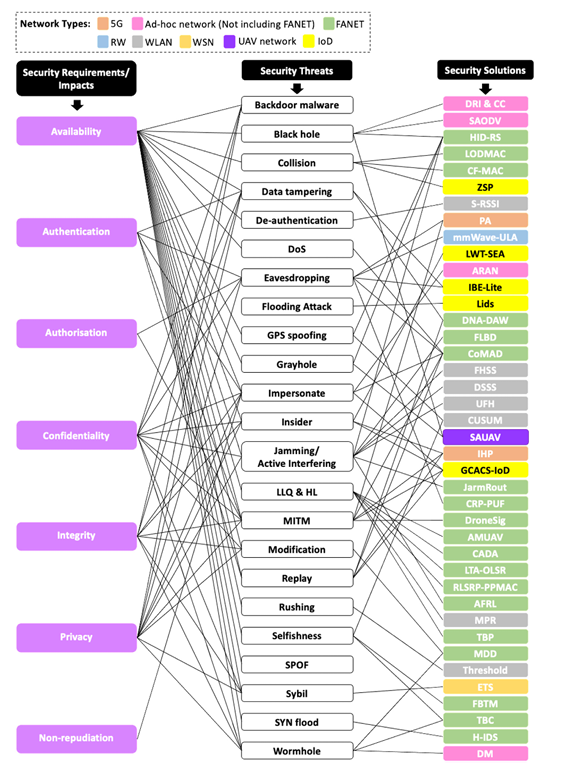
\includegraphics[width=0.7\textwidth]{Figures/Chapter2/Section2/7.png}
        \caption{ Security threats and solutions based on security requirements ~\cite{tsao2022survey}}
        \label{fig:threats_solutions}
    \end{figure}

\subsubsection{Active interfering (jamming)}

Multiple solutions have been developed to address various security threats in FANETs. These include protections against denial of service (DoS), eavesdropping, impersonation, man-in-the-middle (MITM), replay, blackhole and grayhole attacks, GPS spoofing, jamming, collisions, data tampering, and insider threats.

Security methods are generally classified as agent-based or agent-less. Agent-based solutions use device agents, often enhanced by autonomous machine learning algorithms, while agent-less solutions operate without background services. The choice depends on the UAVs’ computational power and application needs.

A security framework outlines twenty-three threats and seven main requirements: availability, confidentiality, privacy, integrity, authentication, authorization, and non-repudiation. Availability stands out as the most critical in FANET environments.

\subsubsection{Backdoormalware}

Currently, there is no specific solution addressing UAV backdoor malware that ensures the confidentiality, availability, integrity, and privacy of FANET communications. While some methods have been developed for mobile nodes in wireless sensor networks, they are not specifically designed for FANET or UAV environments. However, certain techniques involving the detection, tracking, and neutralization of infected nodes may offer potential for addressing future security challenges in UAV networks.


\subsubsection{Blackhole}

The Ad-hoc On-demand Distance Vector (AODV) protocol is vulnerable to blackhole attacks, which can disrupt network integrity. Several solutions have been proposed to enhance FANET availability and prevent packet loss by malicious nodes \cite{sen2011mechanism}.

One solution \cite{sen2011mechanism} uses a secure agent unmanned aerial vehicle (SAUAV) system based on AODV. It operates in two phases: first, identifying and removing malicious UAVs, and second, enabling UAVs to discover neighbors and share information about malicious nodes. This method effectively detects malicious nodes and ensures high packet delivery rates with minimal false positives.

% Another modification to AODV introduces Data Routing Information (DRI) tables and Cross Checking (CC). Each node tracks packet routes through its own DRI. During route discovery, the source node broadcasts a Route Request (RREQ), and an intermediate node responds with a Route Reply (RREP), allowing the source to verify the route's reliability. This helps mitigate blackhole attacks by ensuring only trusted routes are used.

A Secure AODV (SAODV) protocol targets blackhole attacks by ignoring the first reply packet from the source node, assuming malicious nodes reply first. This approach filters out malicious nodes attempting to hijack the route discovery process.

Additionally, a hierarchical detection and response system (HID-RS) uses a centralized Ground Control Station (GCS) to monitor FANET packets. UAVs send neighboring packets to the GCS, which classifies them as normal, suspect, abnormal, or malicious. The GCS then verifies if relay UAVs send packets and calculates dropped packets. A threshold is set and updated with a Support Vector Machine (SVM) to differentiate between intentional and unintentional packet drops.


\subsubsection{Collisions}

UAVs can operate in, join, or leave half-duplex FANET networks, which are characterised by high mobility levels and frequent topology changes. Therefore, the MAC layer must provide collision-free communication and enhance the availability of the FANET. The location-oriented directional MAC protocol (LODMAC) increases FANET capacity and availability by integrating neighbouring UAV locations with directional antennas, resolving issues such as collisions and deafness. A collision-free MAC protocol (CF-MAC) uses the CSMA/TDMA MAC protocol with a half-duplex radio channel and omni-directional antennas. To prevent collisions, time slots are assigned to regulate how UAVs join the network. Additionally, to maintain effective and real-time navigation, only authorised UAVs should operate in specific aerial spaces. UAVs broadcast their location to a zone service provider (ZSP), which detects, monitors, and manages UAV operations, checking for abnormal behaviour, such as denial of service (DoS), spoofing, or data tampering attacks that could disrupt normal network operation.

%%%%%%%%%%%%%%%%%%%%%%%%%%%%%%%%%%%%%%%%%%%%%%%%%%%%%%%%%%%%%%%%%%%%%%

\section{Conclusion}

AI and optimization techniques have revolutionized UAV applications, enabling smarter path planning, resource management, and autonomous decision-making. Reinforcement learning methods like DQN and DDPG have proven particularly effective in handling both discrete and continuous control tasks. However, as UAV networks expand, security threats such as data tampering and denial-of-service attacks demand stronger defenses, including protocols like SAODV and collision-free MAC layers. Future research should focus on lightweight AI models for real-time processing and resilient encryption methods to safeguard UAV communications. This chapter highlights the synergy between AI advancements and security measures, emphasizing both the progress made and the challenges that remain in UAV technology.

\chapter{Traffic monitoring methods}

%%%%%%%%%%%%%%%%%%%%%%%%%%%%% Introduction %%%%%%%%%%%%%%%%%%%%%%%%%%%%%

\section{Introduction}

Traffic monitoring is a critical component of modern urban infrastructure, enabling efficient traffic management, accident prevention, and emergency response. With the rapid growth of urbanization and the increasing complexity of road networks, traditional traffic monitoring systems often struggle to provide real-time, scalable, and cost-effective solutions. In recent years, advancements in Unmanned Aerial Vehicle (UAV) technology and wireless communication systems have opened new possibilities for innovative traffic monitoring approaches. These methods leverage the flexibility, mobility, and adaptability of UAVs to address the limitations of ground-based systems, such as fixed cameras and sensors.

\vspace{\baselineskip} % Add a line space between paragraphs

This chapter explores six distinct methods for UAV-based traffic monitoring, each offering unique solutions to specific challenges in traffic surveillance. From real-time video relay systems to collaborative hotspot selection frameworks, these methods demonstrate the potential of UAVs to enhance traffic monitoring capabilities. The chapter begins with an overview of early systems like the Airborne Traffic Surveillance System (ATSS) and progresses to more advanced approaches, such as 5G-integrated UAV systems and cooperative traffic monitoring using multiple UAVs. Each method is analyzed in terms of its architecture, operational workflow, performance, and limitations, providing a comprehensive understanding of the current state of UAV-based traffic monitoring technologies.

\vspace{\baselineskip} % Add a line space between paragraphs

By examining these methods, this chapter highlights the transformative potential of UAVs in traffic management while also addressing the technical, regulatory, and environmental challenges that must be overcome for widespread adoption. The following sections delve into the details of each method, offering insights into their design, implementation, and real-world applicability.


%%%%%%%%%%%%%%%%%%%%%%%%%%%%% Method 1 %%%%%%%%%%%%%%%%%%%%%%%%%%%%%
\newpage

\section{Method 1: Airborne Traffic Surveillance System (ATSS)}
\label{sec:method1}

In \cite{srinivasan2004atss}, the University of Florida (UFL) research team, in collaboration with the Florida Department of Transportation (FDOT), developed the \textbf{Airborne Traffic Surveillance System (ATSS)}. This innovative system leverages \textbf{Unmanned Aerial Vehicles (UAVs)} and \textbf{microwave IP networks} to transmit highway surveillance data to a \textbf{Base Station (BS)}. The UAV captures video footage of traffic and transmits it in real-time. Two computers located in towers function as video encoders, while another computer at the State Emergency Operations Center receives and displays the strongest video signal. Figure \ref{fig:Methode_1_1} illustrates the system framework.

\begin{figure}[H]  
    \centering
    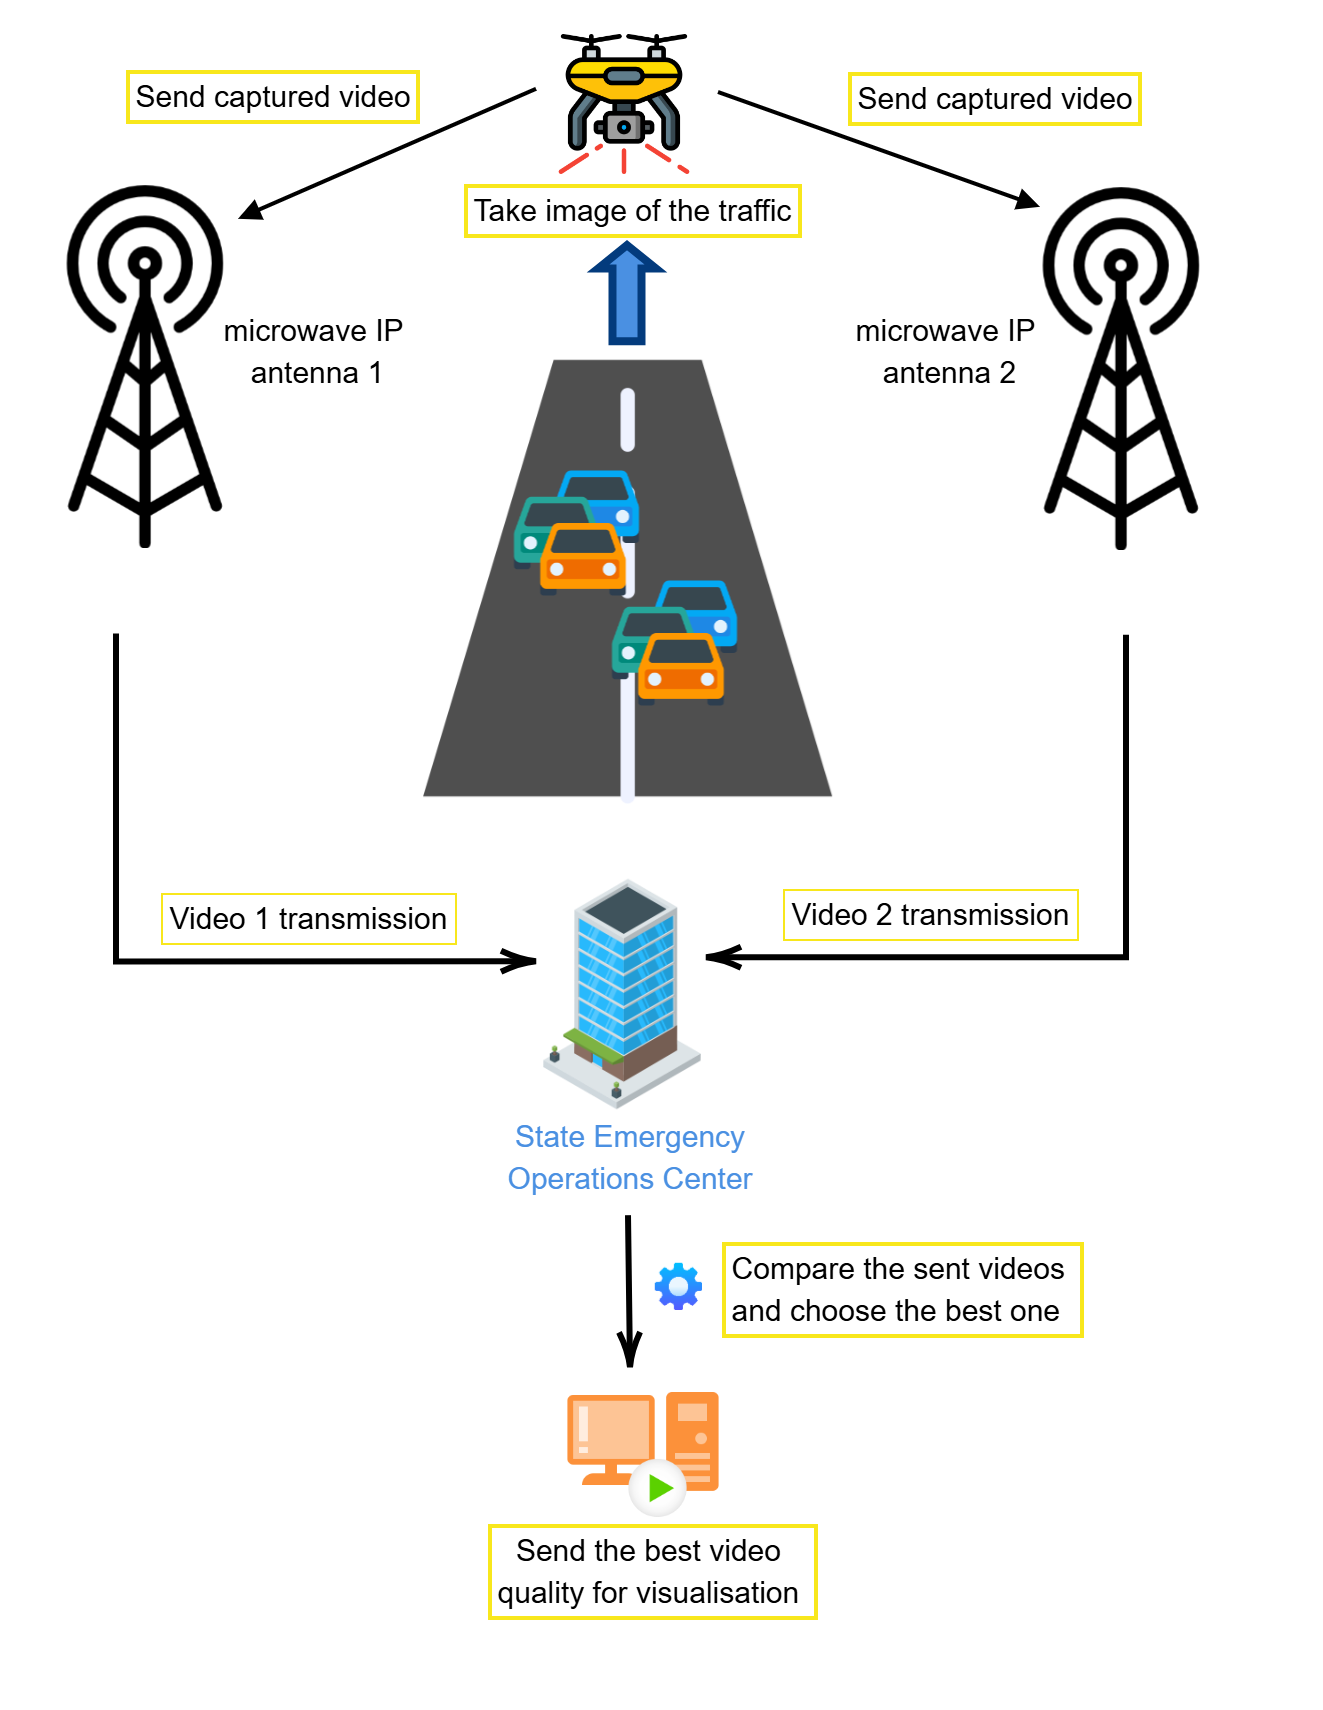
\includegraphics[width=0.7\textwidth]{Figures/Chapter3/Method1/1.png} % Adjust width as needed
    \caption{Airborne Traffic Surveillance System (ATSS) Architecture}
    \label{fig:Methode_1_1} % Reference label
\end{figure}

\subsection{Key Features of ATSS}
The ATSS represents a significant advancement in traffic monitoring, offering the following capabilities:
\begin{itemize}
    \item Real-time video capture and transmission of traffic conditions.
    \item Utilization of UAVs for flexible and scalable surveillance.
    \item Integration with microwave IP networks for data transmission.
    \item Centralized monitoring at the State Emergency Operations Center.
\end{itemize}

\subsection{Limitations of ATSS}
Despite its innovative approach, the ATSS faces several challenges that impact its effectiveness and scalability:
\begin{itemize}
    \item \textbf{Regulatory Constraints:} Federal Aviation Administration (FAA) restrictions limit UAV operations, requiring specific approvals and slowing deployment.
    \item \textbf{Communication Challenges:} Bandwidth limitations, signal reliability issues, and potential interference, especially in adverse weather conditions.
    \item \textbf{Energy and Flight Duration:} Limited battery life necessitates frequent landings and recharging, reducing operational efficiency.
    \item \textbf{Environmental Factors:} Strong winds, rain, and fog degrade video quality and affect UAV stability.
    \item \textbf{Real-Time Video Transmission:} Requires efficient data compression and robust network infrastructure to minimize delays and ensure reliability.
    \item \textbf{Operational Costs:} While more cost-effective than manned aircraft, UAV deployment involves expenses for equipment, trained personnel, and maintenance.
    \item \textbf{Privacy and Security Concerns:} Raises ethical and legal issues, necessitating strict regulations for data collection and surveillance.
\end{itemize}

\subsection{Future Potential}
Despite these limitations, UAV-based traffic monitoring holds significant promise. Future advancements, such as \textbf{AI-driven analysis}, \textbf{improved communication technologies (e.g., 5G)}, and \textbf{autonomous UAV operations}, could enhance its feasibility for large-scale implementation. These developments may address current challenges and unlock new possibilities for real-time traffic management.

\subsection{Conclusion}
The Airborne Traffic Surveillance System (ATSS) represents a pioneering approach to UAV-based traffic monitoring, offering real-time video capture and transmission through microwave IP networks. Despite its innovative design, the system faces challenges such as regulatory constraints, communication limitations, energy inefficiencies, and environmental sensitivities. However, future advancements in AI-driven analytics, 5G communication, and autonomous UAV operations hold the potential to address these limitations, making the ATSS a promising foundation for scalable and efficient traffic surveillance systems.

%%%%%%%%%%%%%%%%%%%%%%%%%%%%% Method 2 %%%%%%%%%%%%%%%%%%%%%%%%%%%%%

\section{Method 2: Video Relay Model Using Public Networks}
\label{sec:method2}

A comparable surveillance method was proposed in \cite{chen2007realtime}, where researchers developed a \textbf{video relay model} using existing public networks. This approach addresses the limitations of traditional traffic surveillance systems, such as the high cost and time-consuming installation of cameras on microwave towers along highways \cite{srinivasan2004atss}. Instead, this method leverages \textbf{mobile broadband connections} to transmit video footage directly to a ground base station (BS) located near the UAV. The efficiency of this method depends on the proximity of ground stations and the availability of a stable broadband network.

\vspace{\baselineskip} % Add a line space between paragraphs

\subsection{Ground Control Station and Network Setup}
A distinctive aspect of this project is the strategic placement of the ground control station near the highway, allowing seamless access to a roadside communication tower. This setup enables the use of the existing mobile broadband network to transmit surveillance video efficiently. The primary goal of video relaying is to send video signals from the UAV ground station in the field to control office computers. Since most of these computers are connected to the Internet, using the public Internet as the main network for video transmission simplifies the setup and reduces system requirements for end-user computers. Figure \ref{fig:method2_architecture} illustrates the proposed architecture.

\vspace{\baselineskip} % Add a line space between paragraphs

\begin{figure}[h]  % 'h' means place the figure "here" if possible
    \centering
    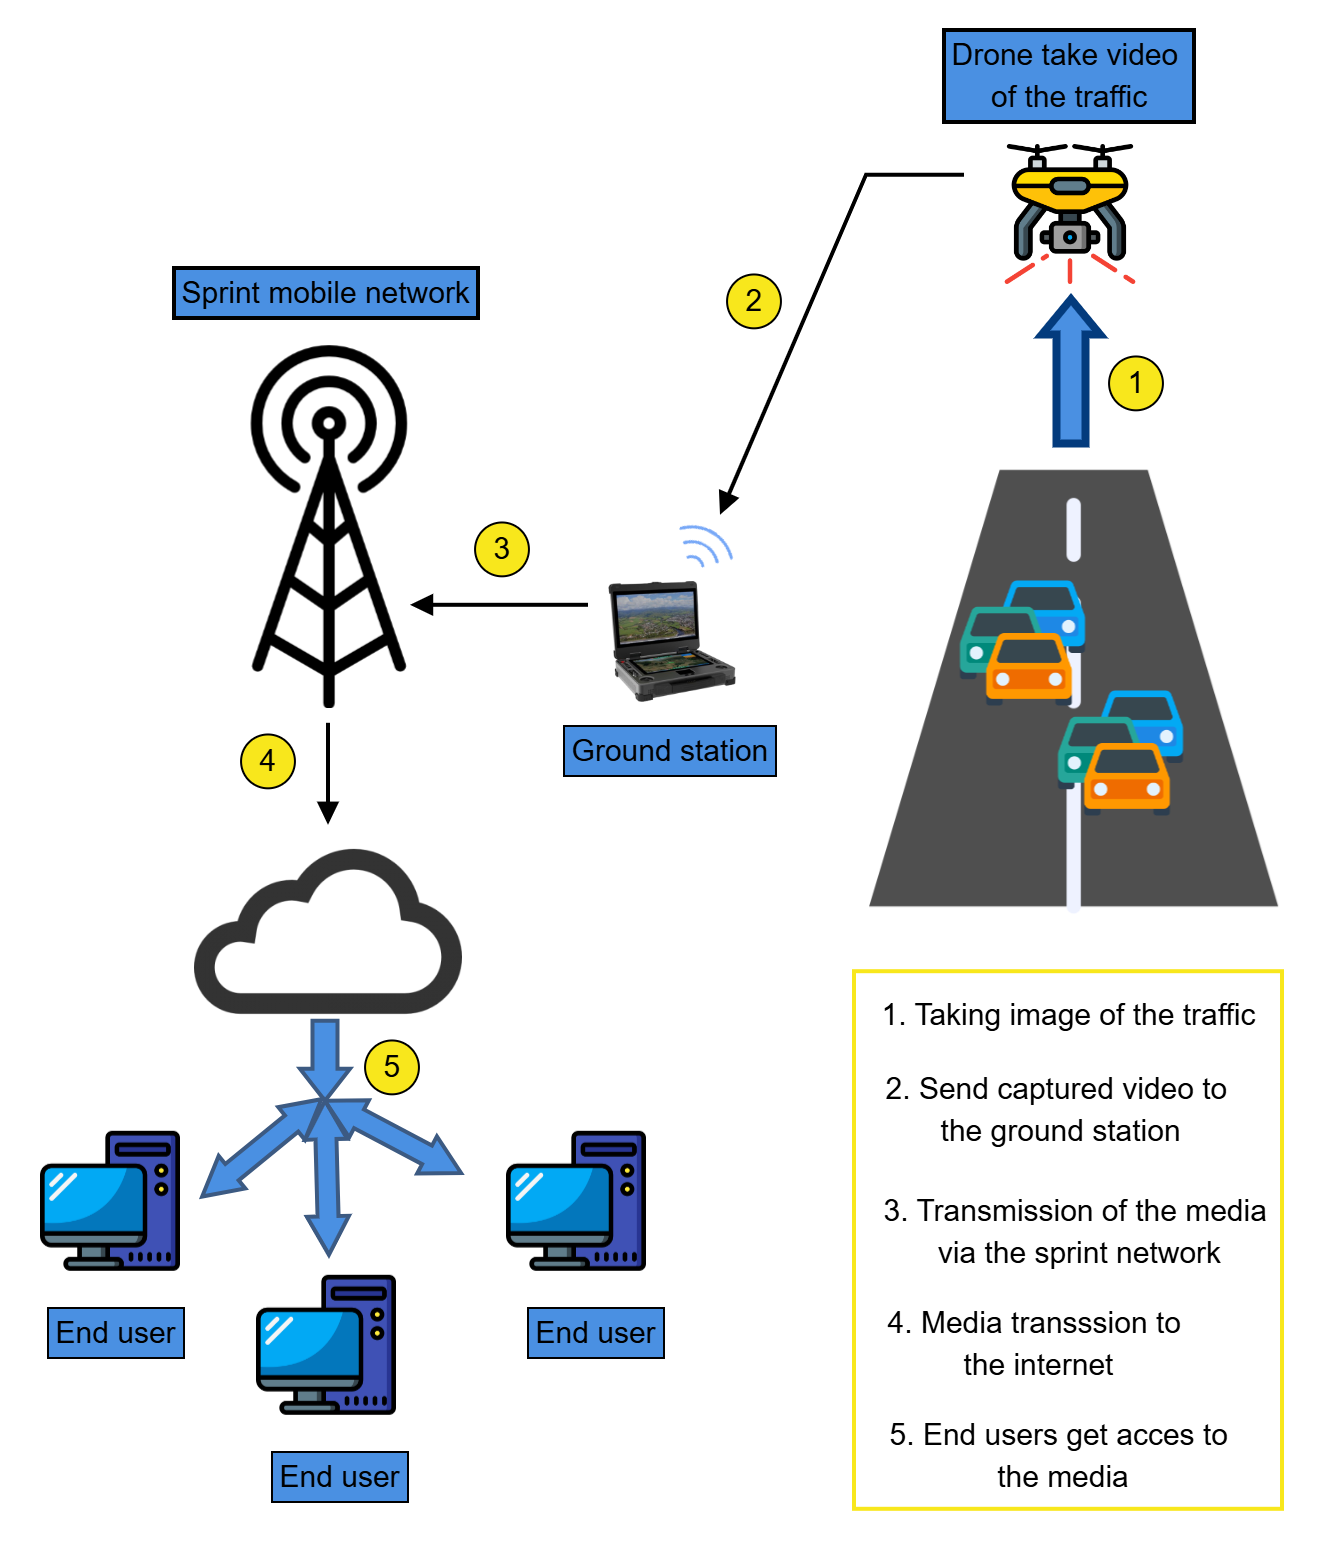
\includegraphics[width=0.7\textwidth]{Figures/Chapter3/Method2/1.png} % Adjust width as needed
    \caption{Proposed Architecture of the Video Relay Model}
    \label{fig:method2_architecture} % Reference label
\end{figure}

\vspace{\baselineskip} % Add a line space between paragraphs

\subsection{Operational Workflow}
The ground station, which consists of a laptop equipped with an antenna, is placed in the field to ensure that the UAV has a suitable flying range covering a section of the Interstate Highway. The best location for the ground station may not always have a wired Internet connection. However, since it is usually set up near the highway, it can take advantage of nearby cellular towers for communication. To send video over the Internet, the UAV ground station uses the nationwide \textbf{Sprint mobile broadband network}. The laptop at the ground station connects to this network using a wireless PC card, which acts as a bridge to the Internet. Once online, the transmitted video is received by the mobile base station through the Internet.

\vspace{\baselineskip} % Add a line space between paragraphs

One drawback of this approach is that the wireless connection in the Sprint mobile broadband network can slow down data transmission. In other words, the system's performance is limited by the available bandwidth in the wireless network. To address this limitation, researchers developed two methods for transmitting the video over the Internet.

\vspace{\baselineskip} % Add a line space between paragraphs

\subsection{Direct IP Address Sharing}
In the first method (see Figure \ref{fig:method2_architecture}), the UAV ground control laptop shares its IP address with end users, who can then use a media player to stream the video from that address. However, the Sprint mobile broadband service assigns a new IP address each time a connection is established. As a result, the IP address changes every time the ground control laptop reconnects to the Sprint network. This requires the ground crew to update and inform end users of the new IP address for each session, creating operational inefficiencies.

\vspace{\baselineskip} % Add a line space between paragraphs

\subsection{Server-Based Video Relay}
An improvement to the system involves using an additional server to manage the data connection. This server has a \textbf{fixed IP address}, which is known in advance by both the UAV ground control laptop and the end-user computers. The UAV ground control laptop streams the video to the server using this fixed IP address, and end users access the video from the same server. Besides real-time streaming, the server can also save the received video for later analysis. Additionally, it hosts the project website, which includes a page displaying the live video feed from the UAV camera. To handle both website hosting and incoming video streams, the server has multiple open network ports. However, using a server may introduce some delays in processing and could be affected by firewall restrictions.

\vspace{\baselineskip} % Add a line space between paragraphs

In this second method, the UAV ground control laptop transmits the video to the server through the mobile broadband network. The server then forwards the video to end-user computers using a wired Internet connection. The number of users who can watch the video at the same time depends on the server's wired connection speed, which is significantly higher than that of the wireless network. As a result, more users can access the video stream simultaneously with a stable data rate. This approach overcomes the limitations of the wireless connection, which is the main bottleneck for video transmission.

\vspace{\baselineskip} % Add a line space between paragraphs

\subsection{Limitations of the Method}
Despite its innovative approach, the video relay model using public networks has several limitations that need to be addressed for practical deployment:

\begin{itemize}
    \item \textbf{Bandwidth Constraints}: The system's performance is heavily dependent on the available bandwidth of the mobile broadband network. In areas with poor network coverage or high congestion, video transmission may suffer from delays or interruptions.
    
    \item \textbf{Operational Inefficiencies}: The direct IP address sharing method requires manual updates to inform end users of new IP addresses, leading to operational inefficiencies and potential delays in accessing video feeds.
    
    \item \textbf{Server Dependency}: The server-based relay method introduces additional complexity and cost. Delays in processing and potential firewall restrictions can impact the system's real-time performance.
    
    \item \textbf{Energy Consumption}: UAVs and ground stations rely on battery power, which limits their operational duration. Frequent recharging or battery replacement may be required, especially in large-scale deployments.
    
    \item \textbf{Environmental Factors}: Adverse weather conditions, such as heavy rain or strong winds, can affect UAV stability and the quality of video footage, reducing the system's reliability.
    
    \item \textbf{Scalability Issues}: While the system performs well in small-scale deployments, scaling it to cover larger areas or higher traffic volumes may introduce challenges in network organization and resource allocation.
\end{itemize}

\vspace{\baselineskip} % Add a line space between paragraphs

\subsection{Conclusion}
In conclusion, the video relay model using public networks represents a \textbf{cost-effective and scalable solution} for UAV-based traffic monitoring. While challenges such as bandwidth limitations and operational inefficiencies persist, the integration of server-based relay systems significantly enhances the method's feasibility and performance.


%%%%%%%%%%%%%%%%%%%%%%%%%%%%% Method 3 %%%%%%%%%%%%%%%%%%%%%%%%%%%%%


\section{Method 3: UAV-Based Traffic Surveillance with 5G Integration}
\label{sec:method3}

In \cite{khan2024smarttraffic}, researchers proposed a novel solution to address the weaknesses of SAHER, an automated traffic enforcement system used in Saudi Arabia. SAHER relies on cameras and radar technology to detect traffic violations such as speeding, running red lights, and lane violations. While effective, the system has several limitations:

\begin{itemize}
    \item Drivers often hide their license plates to avoid detection.
    \item Drivers warn others when they spot a speed camera.
    \item Drivers adhere to speed limits only in areas monitored by SAHER cameras.
    \item Drivers slow down near speed cameras but speed up afterward.
\end{itemize}

To overcome these challenges, the researchers proposed an \textbf{airborne traffic surveillance system} using drones (UAVs) and 5G technology. This system is structured into three layers, each serving a distinct purpose.

\vspace{\baselineskip} % Add a line space between paragraphs

\subsection{System Architecture}
The proposed system consists of three layers:

\begin{itemize}
    \item \textbf{Layer 1}: UAVs fly over highways, capturing video footage and GPS data, which are transmitted to a mobile police base station.
    \item \textbf{Layer 2}: 5G technology ensures a fast and stable connection between the UAVs and the police station.
    \item \textbf{Layer 3}: The system facilitates efficient highway traffic management.
\end{itemize}

\begin{figure}[H]  % 'h' means place the figure "here" if possible
    \centering
    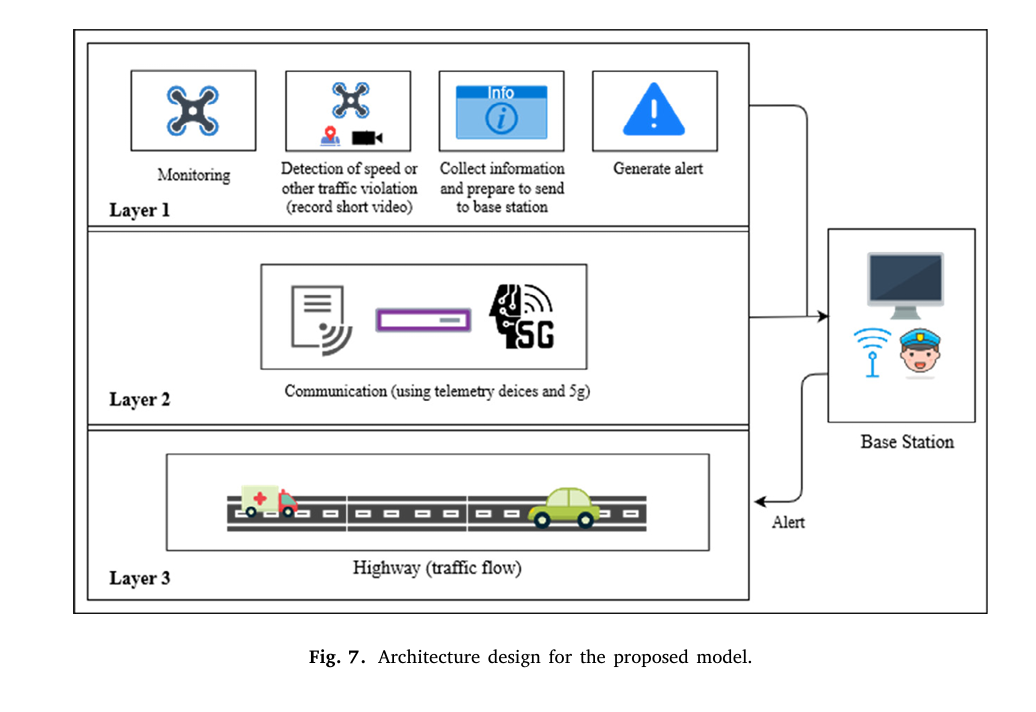
\includegraphics[width=0.7\textwidth]{Figures/Chapter3/Method3/1.png} % Adjust width as needed
    \caption{Proposed Architecture of the UAV-Based Traffic Surveillance System (Source: \cite{khan2024smarttraffic})}
    \label{fig:method3_architecture} % Reference label
\end{figure}

\vspace{\baselineskip} % Add a line space between paragraphs

\subsection{Traffic Monitoring and Violation Detection}
The UAV monitors highway traffic, detects violations, and ensures road safety. When a violation occurs, the system follows a two-step enforcement approach:

\begin{itemize}
    \item \textbf{First Violation}: The UAV issues a warning to the driver through an integrated communication system.
    \item \textbf{Repeated Violation}: If the driver commits the same offense again, the UAV records the details, issues a ticket using License Plate Recognition (LPR), and sends the information to the nearest base station for legal action.
\end{itemize}

\vspace{\baselineskip} % Add a line space between paragraphs

\subsection{Layer 1: UAV-Based Traffic Monitoring}
A UAV is deployed to monitor highways, equipped with an advanced camera and GPS tracking system. It continuously scans traffic for speeding and other infractions, recording real-time violations. When a violation is detected, the UAV captures a short video and logs the GPS coordinates. If it’s the driver’s first offense, the system issues a warning via an integrated module in the vehicle. The collected data is transmitted to the base station for further action. To counteract license plate tampering (e.g., covering plates with tape to evade detection), the base station maintains vehicle records and can take legal action when the vehicle reaches a designated checkpoint.

\vspace{\baselineskip} % Add a line space between paragraphs

\subsection{Layer 2: Communication Network}
This layer facilitates data transmission between the UAV and the base station using telemetry or modern communication technologies. With advancements in communication, \textbf{5G} is the preferred choice due to its high speed, broad coverage, and low latency. The system relies on 5G for seamless and real-time data exchange, ensuring efficient monitoring and response.

\vspace{\baselineskip} % Add a line space between paragraphs

\subsection{Layer 3: Highway Traffic Management}
This layer focuses on optimizing vehicle flow in the monitored areas. By integrating the UAV’s data with traffic control systems, authorities can make informed decisions to improve road safety and efficiency.

\vspace{\baselineskip} % Add a line space between paragraphs

\subsection{Algorithm for Traffic Monitoring}
The following algorithm, adapted from \cite{khan2024smarttraffic}, outlines the process of traffic monitoring and violation detection:




\begin{algorithm}[H]
    \caption{Traffic Monitoring and Rule Violation Detection (Source: \cite{khan2024smarttraffic})}
    \label{alg:traffic_monitoring}
    \textbf{Step 1:} Initialize\;
    
    \textbf{Step 2:} Start monitoring traffic\;
    
    \textbf{Step 3:} Detect speed and other traffic rule violations\;
    
    \textbf{Step 4:} \If{Rule violation found and first time}{
        \textbf{4.1} Generate warning and alert the driver\;
        \textbf{4.2} Record a short video and GPS coordinates\;
        \textbf{4.3} Send video and associated data to ground control station\;
    }
    
    \textbf{Step 5:} \ElseIf{Rule violation found}{
        \textbf{5.1} Record a short video and GPS coordinates\;
        \textbf{5.2} Send video and associated data to ground control station\;
        \textbf{5.3} Ground control station will process data and send to authorities\;
        \textbf{5.4} Go to Step 3\;
    }
    
    \textbf{Step 6:} \If{Flight time ended}{
        \textbf{6.1} Go to Step 8\;
    }
    \Else{
        \textbf{7.1} Go to Step 2\;
    }
    
    \textbf{Step 8:} Go to ground control station\;
    
    \textbf{Step 9:} Exit\;
\end{algorithm}

% \begin{algorithm}[H]
%     \caption{Traffic Monitoring and Rule Violation Detection (Source: \cite{khan2024smarttraffic})}
%     \label{alg:traffic_monitoring}
%     \textbf{Step 1:} Initialize\;
    
%     \textbf{Step 2:} Start monitoring traffic\;
    
%     \textbf{Step 3:} Detect speed and other traffic rule violations\;
    
%     \textbf{Step 4:} \If{Rule violation found and first time}{
%         \textbf{4.1} Generate warning and alert the driver\;
%         \textbf{4.2} Record a short video and GPS coordinates\;
%         \textbf{4.3} Send video and associated data to ground control station\;
%     }
    
%     \textbf{Step 5:} \ElseIf{Rule violation found}{
%         \textbf{5.1} Record a short video and GPS coordinates\;
%         \textbf{5.2} Send video and associated data to ground control station\;
%         \textbf{5.3} Ground control station will process data and send to authorities\;
%         \textbf{5.4} Go to Step 3\;
%     }
    
%     \textbf{Step 6:} \If{Flight time ended}{
%         \textbf{6.1} Go to Step 8\;
%     }
%     \Else{
%         \textbf{7.1} Go to Step 2\;
%     }
    
%     \textbf{Step 8:} Go to ground control station\;
    
%     \textbf{Step 9:} Exit\;
% \end{algorithm}

\vspace{\baselineskip} % Add a line space between paragraphs

\subsection{Limitations of the Proposed System}
Despite its innovative approach, the proposed UAV-based system faces several challenges:

\begin{itemize}
    \item \textbf{Higher Mobility}: The movement of UAVs can cause instability in the communication link, as the network must continuously adjust to their changing positions.
    \item \textbf{Line-of-Sight Interference}: UAVs rely on clear line-of-sight communication, and obstacles like buildings or terrain can block or degrade the signal.
    \item \textbf{Energy Constraints}: The limited battery life of UAVs restricts their ability to operate over long periods, especially in large or remote areas where frequent recharging or battery swaps are required.
\end{itemize}

These factors contribute to the complexity of cellular network planning and make the implementation of this system challenging.

\vspace{\baselineskip} % Add a line space between paragraphs

\subsection{Conclusion}
The proposed UAV-based traffic surveillance system with 5G integration represents a significant advancement in traffic monitoring and enforcement. While challenges such as mobility, line-of-sight interference, and energy constraints persist, the system's potential for real-time monitoring and efficient traffic management makes it a promising solution for future implementation.
    

%%%%%%%%%%%%%%%%%%%%%%%%%%%%% Method 4 %%%%%%%%%%%%%%%%%%%%%%%%%%%%%
 
    
\section{Method 4: Cooperative Traffic Monitoring Using Multiple UAVs}
\label{sec:method4}

In \cite{elloumi2018monitoring}, researchers introduced a cooperative traffic monitoring system using multiple UAVs. This system incorporates two distinct approaches: one focused on maximizing vehicle coverage and the other on detecting various traffic events, such as vehicle positions and speeds. While the first approach dynamically adjusts UAV trajectories based on the movement of targeted vehicle groups, the second relies on predefined vehicle mobility models to determine UAV paths. However, this multi-UAV system lacks real-time capabilities for identifying and reporting speed violations to the mobile police base station.

\vspace{\baselineskip} % Add a line space between paragraphs

\begin{comment}
    

\subsection{System Overview}
The objective of this solution is to track vehicles moving through urban roads, treating them as targets that require continuous monitoring. To design an effective UAV-based system, it is essential to:
\begin{itemize}
    \item Determine a suitable approach for gathering vehicle data.
    \item Strategically position UAVs across the designated area.
    \item Design optimized flight paths to maximize target coverage.
\end{itemize}

The primary challenge lies in determining the number of UAVs required to cover a city, assuming static UAV placement. Since deploying an unlimited number of UAVs is impractical, each UAV must cover multiple targets. One way to reduce the number of UAVs is by clustering targets and assigning one UAV to each cluster. This approach is similar to techniques used in sensor networks or Vehicular Ad-Hoc Networks (VANETs). Key parameters for clustering include target distances, velocities, and movement directions. A group is more stable if its members have similar velocities and move in the same direction.


\end{comment}



\vspace{\baselineskip} % Add a line space between paragraphs

\subsection{Key Components of the System}
The system is constracted through three main steps:

\subsubsection{Collecting Information About Vehicles}
Various parameters can be monitored and measured based on the devices deployed over the coverage area, including:
\begin{itemize}
    \item Vehicle position, speed, and direction.
    \item The number of vehicles in an area.
    \item The number of vehicles passing through specific points, such as intersections or crossings.
\end{itemize}

Specific events, such as speeding or traffic jams, are identified by changes in these parameters. For example:
\begin{itemize}
    \item Speeding is detected when a vehicle exceeds a set speed limit.
    \item Traffic jams are identified when the speed of multiple vehicles drops below a certain threshold.
\end{itemize}

In this research, \cite{elloumi2018monitoring} consider multiple UAVs equipped with image-processing capabilities that enable them to accurately measure these parameters. The UAVs are assumed to:
\begin{itemize}
    \item Always detect targets within their field of view, with no obstacles obstructing their line of sight.
    \item Temporarily adjust their altitude to avoid collisions.
    \item Exchange information about the vehicles they are tracking, including identifiers and positions.
\end{itemize}

\vspace{\baselineskip} % Add a line space between paragraphs

\subsubsection{Deploying UAVs Over Coverage Areas}
The key challenge is determining the number of UAVs required to effectively cover a city area. Since deploying an unlimited number of UAVs is impractical, each UAV must monitor multiple targets. To minimize the required number of UAVs, targets are grouped into clusters, with each UAV assigned to a specific cluster. The clustering process considers factors such as:
\begin{itemize}
    \item Distance between targets.
    \item Velocities of targets.
    \item Movement directions of targets.
\end{itemize}

An off-line algorithm (Algorithm 1) is proposed for this clustering, allowing system operators to estimate the UAV count. The algorithm inputs are shown in Table \ref{tab:clustering_inputs}. Three criteria are used for clustering:
\begin{itemize}
    \item Distance between the central target and potential group members (mandatory).
    \item Speed difference between targets (optional).
    \item Direction of movement (optional).
\end{itemize}

\begin{table}[H]
    \centering
    \begin{tabular}{|l|l|}
    \hline
    \textbf{Abbreviation} & \textbf{Description} \\ \hline
    Tnb & Targets numbers \\ \hline
    G & Groups members \\ \hline
    D & Max distance value \\ \hline
    V & Max speed difference \\ \hline
    Pt & Target position \\ \hline
    Mt & Target direction \\ \hline
    Vt & Target velocity \\ \hline
    compt & Covered targets \\ \hline
    Ttag & Target tag \\ \hline
    Tid & Target id \\ \hline
    Cid & Central target id \\ \hline
    Pc & Central target position \\ \hline
    Mc & Central target direction \\ \hline
    Ctag & Central target tag \\ \hline
    Vc & Central target speed \\ \hline
    \end{tabular}
    \caption{Input Parameters for Clustering Algorithm (Source: \cite{elloumi2018monitoring})}
\end{table}


\vspace{\baselineskip} % Add a line space between paragraphs

\begin{algorithm}[H]
    \caption{Clustering Algorithm}
    \label{alg:uniform_method}
    
    \textbf{Step 1:} Initialize $j \gets 1$, $\text{compt} \gets 0$\;
    
    \textbf{Step 2:} \While{$\text{compt} < T_{\text{nb}}$}{
        \textbf{2.1} \While{$C_{\text{tag}}(j) = 1$}{
            \textbf{2.1.1} Sample $P_c(j) \sim \text{Uniform}(P_t)$\;
            
            \textbf{2.1.2} Set $C_{\text{tag}}(j) \gets 1$\;
            
            \textbf{2.1.3} Set $G(j, j) \gets C_{\text{id}}(j)$\;
            
            \textbf{2.1.4} Increment $\text{compt} \gets \text{compt} + 1$\;
            
            \textbf{2.1.5} \For{$i = 1$ \KwTo $T_{\text{nb}}$}{
                \textbf{2.1.5.1} \If{$(T_{\text{tag}}(i) = 0) \land (i \neq j)$}{
                    \textbf{2.1.5.1.1} \If{$M_t(i) = M_c(j)$}{
                        \textbf{2.1.5.1.1.1} \If{$|V_t(i) - V_c(j)| < V$}{
                            \textbf{2.1.5.1.1.1.1} \If{$|P_t(i) - P_c(j)| < D$}{
                                \textbf{2.1.5.1.1.1.1.1} Set $G(j, i) \gets T_{\text{id}}(i)$\;
                                
                                \textbf{2.1.5.1.1.1.1.2} Increment $\text{compt} \gets \text{compt} + 1$\;
                                
                                \textbf{2.1.5.1.1.1.1.3} Set $T_{\text{tag}}(i) \gets 1$\;
                            }
                        }
                    }
                }
            }
            
            \textbf{2.1.6} Increment $j \gets j + 1$\;
        }
    }
    
    \textbf{Step 3:} End\;
\end{algorithm}

    

% \begin{algorithm}[H]
% \caption{Clustering Algorithm (Source: \cite{elloumi2018monitoring})}
% \label{alg:uniform_method}
% \begin{algorithmic}[1]
% \State $j = 1$; $\text{compt} = 0$;
% \While{$\text{compt} < T_{\text{nb}}$}
%     \While{$C_{\text{tag}}(j) == 1$}
%         \State $\bigcup\limits_{c(j)} P_c(j) = \text{Uniform } (P_t)$;
%         \State $C_{\text{tag}}(j) = 1$; $G(j, j) = C_{\text{id}}(j)$;
%         \State $\text{compt} = \text{compt} + 1$;
%         \For{$i = 1$ to $T_{\text{nb}}$}
%             \If{$(T_{\text{tag}}(i) == 0) \& (i \neq j)$}
%                 \If{$(M_t(i) == M_c(j))$}
%                     \If{$|V_t(i) - V_c(j)| < V$}
%                         \If{$|P_t(i) - P_c(j)| < D$}
%                             \State $G(j, i) = T_{\text{id}}(i)$;
%                             \State $\text{compt} = \text{compt} + 1$;
%                             \State $T_{\text{tag}}(i) = 1$;
%                         \EndIf
%                     \EndIf
%                 \EndIf
%             \EndIf
%         \EndFor
%         \State $j = j + 1$;
%     \EndWhile
% \EndWhile
% \end{algorithmic}
% \end{algorithm}


\subsubsection{Designing UAV Trajectories}
Once the number of UAVs is estimated, the next step is to design their trajectories. Three different approaches are explored:

\begin{itemize}
    \item \textbf{Fixed Trajectory Approach} This method relies on predetermined UAV paths guided by fixed Points of Interest (POIs), such as busy intersections or high-traffic zones. A single UAV is used to monitor these areas.
    \item \textbf{Mobile POI Approach} This method incorporates multiple cooperative UAVs. Each UAV detects targets within its field of view (FoV), estimates their positions and speeds, and shares this data with other UAVs and a central system. Unlike the fixed trajectory approach, both UAV trajectories and POIs are dynamic. The objective is to maximize the number of targets in a UAV's FoV for the longest possible duration.
    \item \textbf{Vehicular Mobility-Based Approach} This method leverages vehicular mobility models to determine UAV trajectories. Multiple UAVs are deployed, following the Shortest Path Map-Based Movement model, which aligns their paths with road networks to enhance observation opportunities. UAV speeds are adjusted to match those of the observed vehicles.
\end{itemize}



\begin{figure}[H]
    \centering
    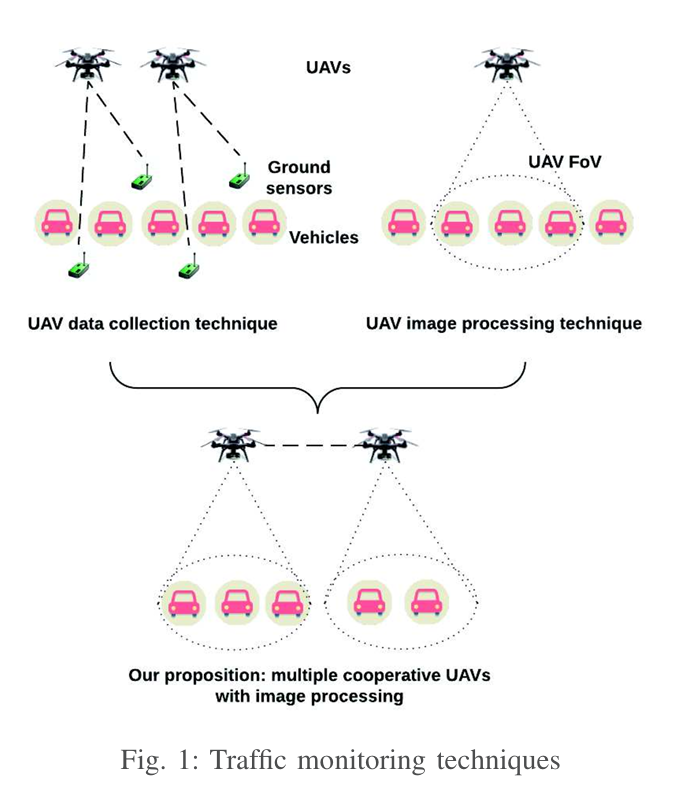
\includegraphics[width=0.7\textwidth]{Figures/Chapter3/Method4/3.png}
    \caption{Traffic monitoring techniques (Source: \cite{elloumi2018monitoring})}
    \label{fig:vehicular_mobility}
\end{figure}

\vspace{\baselineskip} % Add a line space between paragraphs

\subsection{Simulation and Results}
The study evaluates UAV-based road traffic monitoring (RTM) through simulations. Real-world taxi mobility datasets from Rome and San Francisco were initially considered but deemed unsuitable due to sparse vehicle distribution. Instead, the Opportunistic Network Environment (ONE) simulator was used to generate vehicle movement patterns based on real maps, applying Dijkstra’s shortest path algorithm. The research tested different UAV clustering methods based on distance, velocity, and direction to optimize monitoring. Simulations examined UAV coverage efficiency, event detection (speeding, congestion), and tracking methods.

\subsubsection{Key Findings}
\begin{itemize}
    \item \textbf{Fixed POI Method with Random UAV Movement}: The detection rate of speeding vehicles increases from 32\% (5 POIs) to 80.87\% (50 POIs). However, as the number of POIs increases, the time UAVs spend over a given area decreases, leading to shorter detected event durations.
    \item \textbf{Mobile Trajectory Methods}: These methods perform better, achieving up to 28.62\% coverage (Mobile POI with 50 UAVs) and a 30.09\% speeding violation detection rate (Vehicular Mobility-Based Method with 50 UAVs). Since UAVs follow mobile trajectories rather than fixed points, they can track events more accurately over time.
    \item \textbf{Impact of UAV Numbers}: For a small number of UAVs, all methods perform similarly. However, from 25 UAVs onward, the proposed methods show significant improvement. The initial estimate was that 25 UAVs would cover 10\% of targets, but with the proposed methods, the coverage rate reaches 17\%.
\end{itemize}

This table compares three UAV trajectory methods: the \textbf{Fixed Trajectory Approach}, the \textbf{Mobile POI Method}, and the \textbf{Vehicular Mobility-Based Method}. It highlights key differences in target tracking, adaptation, application domains, and UAV speed, showcasing how each approach is suited for specific monitoring tasks such as traffic surveillance, crowd tracking, or animal monitoring.

\begin{table}[H]
    \centering
    \begin{tabular}{|p{3cm}|p{4cm}|p{4cm}|p{4cm}|}
        \toprule
        \textbf{Criterion} & \textbf{Fixed Trajectory} & \textbf{Mobile POI} & \textbf{Vehicular Mobility} \\
        & \textbf{Approach} & \textbf{Method} & \textbf{Based Method} \\
        \midrule
        \textbf{Target Tracking} & Fixed Points of Interest (POIs) & Center of gravity of target groups & Pre-calculated trajectories on roads \\
        \midrule
        \textbf{Adaptation} & Static, predefined paths & Dynamic, based on target movements & Static, follows pre-generated points \\
        \midrule
        \textbf{Application Domain} & High-traffic zones (e.g., intersections) & Crowd monitoring, animal tracking, etc. & Traffic monitoring \\
        \midrule
        \textbf{UAV Speed} & Fixed & Variable, depending on group movements & Adjusted to match vehicle speeds \\
        \bottomrule
    \end{tabular}
    \caption{Comparison of Fixed Trajectory, Mobile POI, and Vehicular Mobility Based Methods}
    \label{tab:comparison_uav}
\end{table}

\vspace{\baselineskip} % Add a line space between paragraphs

\subsection{Limitations of the Method}
Despite its innovative approach, the proposed cooperative traffic monitoring system using multiple UAVs has several limitations:

\begin{itemize}
    \item \textbf{Real-Time Reporting}: The system lacks real-time capabilities for identifying and reporting speed violations to the mobile police base station. This limits its effectiveness in enforcing traffic regulations promptly.
    \item \textbf{Energy Constraints}: UAVs have limited battery life, which restricts their operational duration and requires frequent recharging or battery swaps, especially in large or remote areas.
    \item \textbf{Communication Challenges}: Maintaining stable communication links between UAVs and the ground station can be difficult, particularly in urban environments with obstacles that block or degrade signals.
    \item \textbf{Scalability Issues}: While the system performs well with a moderate number of UAVs, scaling it up to cover larger areas or more targets may require significant computational and logistical resources.
    \item \textbf{Environmental Factors}: Adverse weather conditions, such as strong winds or heavy rain, can affect UAV stability and the quality of video footage, reducing the system's reliability.
\end{itemize}

\vspace{\baselineskip} % Add a line space between paragraphs

\subsection{Conclusion}
The proposed cooperative traffic monitoring system using multiple UAVs demonstrates significant potential for urban traffic management. While challenges such as real-time speed violation reporting, energy constraints, and scalability persist, the integration of dynamic trajectory planning and clustering techniques enhances the system's effectiveness. Future work could focus on improving real-time capabilities, extending UAV battery life, and addressing communication challenges to enable large-scale implementation.

    

%%%%%%%%%%%%%%%%%%%%%%%%%%%%% Method 5 %%%%%%%%%%%%%%%%%%%%%%%%%%%%%


\section{Method 5: UAV-Assisted Emergency Vehicle Routing}
\label{sec:method5}

In a distinct approach, \cite{oubbati2019leveraging} proposed a UAV-based system specifically designed to assist emergency vehicles, such as ambulances, in identifying the optimal route through traffic to reach incident sites. The system is structured into four primary components:
\begin{itemize}
    \item \textbf{Weighting of Road Segments}: Based on traffic fluidity.
    \item \textbf{Network Organization}: Establishing a robust and energy-efficient backbone among UAVs.
    \item \textbf{Reactive Routing}: Deploying communication between the Area of Interest (AoI) and relevant services.
    \item \textbf{Path Calculation}: Determining the near-optimal path in terms of travel time to the AoI.
\end{itemize}

\vspace{\baselineskip} % Add a line space between paragraphs

\subsection{System Overview}
The proposed system enables UAVs to analyze nearby road segments and track changes in traffic conditions. UAVs communicate and collaborate by:
\begin{itemize}
    \item Exchanging messages to organize their network.
    \item Overseeing road activity to detect incidents.
    \item Promptly notifying appropriate services to support intervention.
\end{itemize}

\vspace{\baselineskip} % Add a line space between paragraphs

\subsection{System Composition}
The system is composed of \( n \) UAVs distributed across a three-dimensional (3D) space, moving randomly above various road segments. Key features of the UAVs include:
\begin{itemize}
    \item \textbf{Initial State}: Each UAV starts with a fully charged battery.
    \item \textbf{Movement Parameters}: UAVs have access to their position, speed, direction, and information about nearby UAVs.
\end{itemize}

\vspace{\baselineskip} % Add a line space between paragraphs

\subsection{UAV States and Communication}
UAVs operate in one of two states:
\begin{itemize}
    \item \textbf{Normal UAV}: Performs standard monitoring tasks.
    \item \textbf{Backbone UAV}: Acts as a communication relay for the network.
\end{itemize}

Communication between UAVs and ground vehicles is facilitated using the \textbf{IEEE 802.11p} wireless standard. To address energy constraints, the authors define three distinct levels of remaining battery capacity:
\begin{itemize}
    \item \textbf{High}: 66–100\% remaining energy.
    \item \textbf{Medium}: 33–66\% remaining energy.
    \item \textbf{Low}: 0–33\% remaining energy.
\end{itemize}

\vspace{\baselineskip} % Add a line space between paragraphs

\subsection{Operational Constraints}
Each UAV has the following operational constraints:
\begin{itemize}
    \item \textbf{Line-of-Sight (LoS) Range}: Up to 300 meters.
    \item \textbf{Altitude}: Operates at low altitudes, remaining below 300 meters.
    \item \textbf{Incident Detection}: Under clear weather conditions, UAVs can detect road incidents using image processing techniques. However, the specifics of image analysis fall outside the scope of this work.
\end{itemize}

\vspace{\baselineskip} % Add a line space between paragraphs

\subsection{Weight Calculation}
To determine the weight of a road segment, the hovering UAV collects Hello packets that are periodically exchanged between vehicles. Each intercepted Hello packet contains movement information, including the vehicle's position and speed. Regardless of its energy level or state, the UAV maintains a monitoring table to track traffic density, updating it as it receives Hello packets from vehicles traveling on a given road segment.

As illustrated in Table~\ref{tab:monitoring_table}, four UAVs (\( u_1, u_2, u_3, u_4 \)) monitor Hello packet exchanges from vehicles on four distinct road segments, each divided into three fixed zones. For instance, the monitoring table of UAV \( u_3 \) (Table~\ref{tab:monitoring_table}) is used to compute key parameters required to determine the weight of the road segment between intersections \( I_X \) and \( I_Z \).

\begin{table}[H]
    \centering
    \caption{Monitoring table of UAV \( u_3 \) (adapted from \cite{oubbati2019leveraging})}
    \label{tab:monitoring_table}
    \begin{tabular}{|c|c|c|}
        \hline
        \textbf{Zone} & \textbf{Vehicle (Position (x,y))} & \textbf{Speed (m/s)} \\
        \hline
        Zone 1 & \( v_1 \) (100.00, 5.00) & 10 \\
        \hline
        Zone 2 & \( v_2 \) (90.00, 305.00) & 8 \\
               & \( v_3 \) (90.00, 405.00) & 8 \\
        \hline
        Zone 3 & \( v_4 \) (90.00, 505.00) & 8 \\
               & \( v_5 \) (100.00, 610.00) & 14 \\
        \hline
    \end{tabular}
\end{table}

The total number of vehicles on segment \( S_{I_X I_Z} \) is given by:
\begin{equation}
    T_{S_{I_X I_Z}} = 5, \quad SP_{av} = 96 \text{ m/s}
\end{equation}

The traffic density regulation is assessed by computing the standard deviation, which reflects how vehicles are distributed across a given road segment:
\begin{equation}
    \sigma_{S_{I_i I_j}} = \sqrt{\frac{1}{S_{I_i I_j}} \sum_{i=1}^{S_{I_i I_j}} T_{Zone_i}^2 }
\end{equation}
where:
\begin{itemize}
    \item \( T_{S_{I_i I_j}} \) is the total number of vehicles in the road segment \( S_{I_i I_j} \) between intersections \( I_i \) and \( I_j \).
    \item \( \overline{T_{Zone}} \) is the average number of vehicles per zone.
    \item \( T_{Zone_i} \) is the number of vehicles in zone \( Zone_i \).
    \item \( S_{I_i I_j} \) is the number of fixed zones in the road segment \( S_{I_i I_j} \).
\end{itemize}

If \( \sigma = 0 \), vehicles are evenly distributed, implying free traffic flow. Otherwise, if \( \sigma > 0 \), vehicles tend to cluster, often due to traffic lights or congestion.

The weight of a segment \( S_{I_i I_j} \) is calculated as:
\begin{equation}
    \text{Weight} = \frac{T_{S_{I_i I_j}} +1}{d_{I_i I_j}} \times \frac{1}{SP_{av} +1}
\end{equation}
where \( d_{I_i I_j} \) is the segment length. The weight is directly proportional to \( T_{S_{I_i I_j}} \) and \( d_{I_i I_j} \). The computed weight is always non-negative and provides an indicator of traffic conditions: lower weight values correspond to better road segments.

Table~\ref{tab:weight_calculation} presents the computed weight values for different segments.

\begin{table}[H]
    \centering
    \caption{Weight Calculation Scenario (adapted from \cite{oubbati2019leveraging})}
    \label{tab:weight_calculation}
    \begin{tabular}{|c|c|c|c|c|}
        \hline
        \textbf{Segment} & \( d_{I_i I_j} \) (m) & \( T_{S_{I_i I_j}} \) & \( SP_{av} \) (m/s) & \textbf{Weight} \\
        \hline
        \( S_{I_X I_Z} \) & 1500 & 5 & 10 & 463.82 \\
        \( S_{I_Z I_Y} \) & 1500 & 0 & 0 & 0.00 \\
        \( S_{I_Y I_W} \) & 1500 & 2 & 14 & 136.05 \\
        \( S_{I_W I_X} \) & 1500 & 12 & 0 & 7468.87 \\
        \hline
    \end{tabular}
\end{table}

The segment \( S_{I_Z I_Y} \) has the lowest weight and is thus the most suitable for emergency vehicle traversal.

\vspace{\baselineskip} % Add a line space between paragraphs

\subsection{Organization and Data Routing}
To address the complexity of making a stable and reliable data transmission for alert messages, a stable backbone network is established by considering both UAV connectivity and their remaining energy levels. Graph-based modeling simplifies backbone construction by leveraging established graph theory algorithms. In this approach, UAVs and target services are represented as an undirected graph \( G(V,E) \), where \( V \) denotes vertices (UAVs and services), and \( E \) represents bidirectional links between them at a given time \( t \).

\vspace{\baselineskip} % Add a line space between paragraphs

\begin{figure}[H]
    \centering
    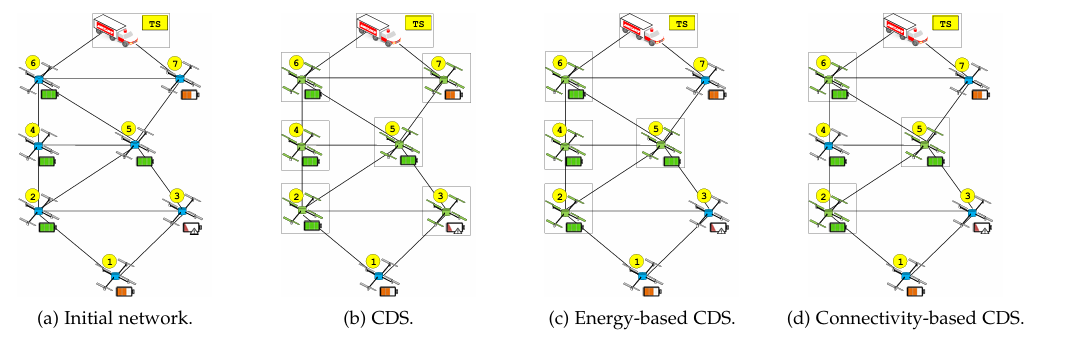
\includegraphics[width=0.7\textwidth]{Figures/Chapter3/Method5/1.png}
    \caption{Connected dominating set (CDS) formation (Source: \cite{oubbati2019leveraging})}
    \label{fig:CDS}
\end{figure}




\subsection{Connected Dominating Set (CDS) Formation}
A Connected Dominating Set (CDS) is a subset \( D \) of vertices where each non-member is connected to at least one node in \( D \), and all members of \( D \) are interconnected. Figure~\ref{fig:CDS} illustrates this process. UAVs periodically exchange Hello packets (Fig.~\ref{fig:Hello_packet_format}), which contain their ID, remaining energy (RE), mobility data (position, speed, velocity), and neighboring nodes. These details help calculate link connectivity lifetime and define network segments. A flag in the packet indicates whether a UAV belongs to the backbone (1) or not (0).

To construct the CDS, a marking process is applied:
\begin{itemize}
    \item All UAVs are initially unmarked, except the Target Service (TS), which is permanently marked.
    \item Each UAV shares its neighbor list.
    \item UAVs with two unconnected neighbors are marked.
\end{itemize}

This results in a subgraph \( M \), where \( M = G[D] \), ensuring two key properties:
\begin{itemize}
    \item \textbf{Property 1}: \( D \) forms a dominating set in \( G \).
    \item \textbf{Property 2}: \( M \) remains a connected subgraph.
\end{itemize}

Since minimizing a CDS is NP-complete, we refine \( D \) using two rules:
\begin{itemize}
    \item \textbf{Rule 1}: If a UAV \( u_i \) has a subset of its neighbors covered by another UAV \( u_j \) and \( RE_{u_i} < RE_{u_j} \), then \( u_i \) is removed from \( M \).
    \item \textbf{Rule 2}: If \( u_i \) has a lower average connectivity lifetime (ACL) than \( u_j \), it is removed. ACL is calculated using the estimated connectivity duration between UAVs.
\end{itemize}

Applying these rules optimizes the CDS, ensuring long-term connectivity while maintaining a stable backbone. The CDS updates continuously through Hello packet exchanges, providing robust network reliability.

\begin{figure}[H]
    \centering
    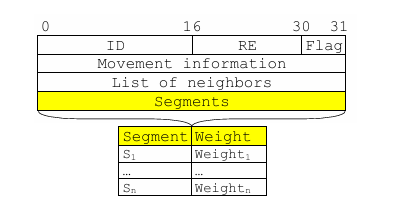
\includegraphics[width=0.7\textwidth]{Figures/Chapter3/Method5/2.png}
    \caption{Hello packet format (Source: \cite{oubbati2019leveraging})}
    \label{fig:Hello_packet_format}
\end{figure}

\vspace{\baselineskip} % Add a line space between paragraphs

\subsection{Routing}
Once the CDS is defined, an innovative routing strategy is implemented to ensure communication between the UAVs and the relevant services. This reactive approach considers two essential aspects:
\begin{itemize}
    \item Excluding UAVs with low energy levels to preserve their autonomy.
    \item Selecting routes based on link stability.
\end{itemize}

\subsubsection{Packet Format}
The RREQ (Route Request) packet contains several fields:
\begin{itemize}
    \item Transmission ID: identifier of the discovery process.
    \item NS: number of segments traversed.
    \item DelayP: transmission delay to the target service (TS).
    \item Source / TS: identifiers of the communicating nodes.
    \item Movement information: used to estimate the connection duration between UAVs.
    \item CLP (connectivity lifetime path): minimum connection duration between the UAVs in the path.
    \item REP (residual energy path): minimum energy level of the UAVs in the path.
    \item Distance: total number of UAVs traversed.
\end{itemize}

The RREP (Route Reply) packet includes these fields to inform the source about the status of the selected path. Once the RREP is received, alert transmission can begin.

\subsubsection{Routing Process}
Consider the example of an accident detected on a road. The nearest UAV immediately sends an alert to a backbone UAV, \( u_1 \). This alert contains a unique identifier, location (AoI), and the nature of the incident. Initially, only the road segments detected by the source UAV are recorded.

The UAV \( u_1 \) then broadcasts an RREQ packet to find a path to TS (hospital). At each step, information about link stability and residual UAV energy is collected. To avoid redundancies, an RREQ that has already been received with the same Transmission ID is ignored.

As soon as the first RREQ reaches TS, a short delay allows the accumulation of all available responses before selecting the optimal route. The path is chosen based on a multi-criteria score considering available energy (REP), connection duration (CLP), and number of segments traversed (NS), according to the following equation:

\[
Score = \frac{REP \times NS}{Distance} \times \frac{CLP}{DelayP}
\]

A high score indicates a reliable and stable route. Path1 (\( u_1 \rightarrow u_2 \rightarrow u_4 \rightarrow u_5 \rightarrow TS \)) is selected as it offers the best performance.


\begin{figure}[H]
    \centering
    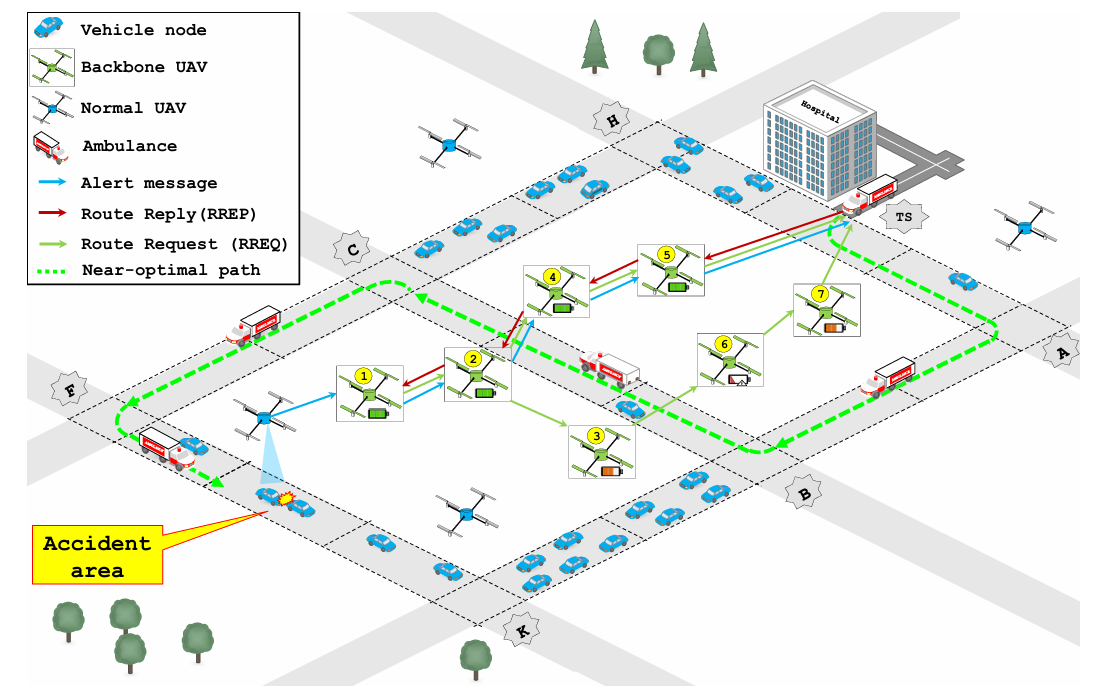
\includegraphics[width=0.7\textwidth]{Figures/Chapter3/Method5/4.png}
    \caption{alert model functioning (Source: \cite{oubbati2019leveraging})}
    \label{fig:Hello_packet_format}
\end{figure}

\subsubsection{Optimal Path Calculation to the Incident}
Once the alert is transmitted to TS, it has precise information about the incident and surrounding traffic density. Based on the weights assigned to road segments, TS calculates the best ground route to reach the AoI, ensuring a rapid emergency response.

\vspace{\baselineskip} % Add a line space between paragraphs

\subsection{Performance Evaluation}
The performance of the proposed application is evaluated through a series of experiments using NS-2, SUMO, and MobiSim for mobility generation. A test urban area of \(3 \times 3 \, \text{km}^2\) is imported from OpenStreetMap, with relevant road segments and intersections marked for simulation. Key simulation parameters are summarized in Table~\ref{tab:sim_params}.

\begin{table}[H]
    \centering
    \caption{Simulation Parameters}
    \label{tab:sim_params}
    \begin{tabular}{|l|l|}
        \hline
        \textbf{Parameter} & \textbf{Value} \\
        \hline
        Frequency Band & 5.9 GHz \\
        Transmit Power & 21.5 dBm \\
        Sensitivity & -81.5 dBm \\
        MAC Layer & IEEE 802.11p \\
        Data Rate & 1 Mbit/s \\
        Area Size & \(3 \times 3 \, \text{km}^2\) \\
        Simulation Time & 300 s \\
        Number of UAVs & [10, 100] \\
        Number of Vehicles & 100 \\
        UAV Altitude & 300 m \\
        Communication Range & 300 m \\
        Hello Interval & 0.1 s \\
        Initial Energy of UAVs & 2000 J \\
        \hline
    \end{tabular}
\end{table}

\subsubsection{Routing Performance}
Three metrics are evaluated: Packet Delivery Ratio (PDR), End-to-End Delay (EED), and Overhead (OH). The proposed routing protocol is compared with LAROD and MPGR. Results show that:
\begin{itemize}
    \item \textbf{PDR}: The proposed protocol outperforms others, increasing PDR by more than 20\% due to efficient backbone utilization.
    \item \textbf{EED}: The average delay is minimized as UAV density increases, thanks to energy-rich and well-connected routing paths.
    \item \textbf{OH}: Control overhead decreases with higher UAV density, as fewer route discoveries are needed.
\end{itemize}

\subsubsection{Energy Consumption Performance}
The remaining energy levels of 50 UAVs are analyzed. The proposed protocol demonstrates well-regulated energy consumption, as it relies on backbone UAVs with high energy levels. In contrast, LAROD and MPGR show unbalanced energy consumption, with some UAVs consuming up to 60\% more energy.

\subsubsection{Application Performance}
Experiments focus on road segment coverage, backbone UAVs, and ambulance travel time:
\begin{itemize}
    \item \textbf{Coverage}: Full road segment coverage is achieved with approximately 70 UAVs.
    \item \textbf{Backbone UAVs}: The number of backbone UAVs increases uniformly with UAV density.
    \item \textbf{Travel Time}: The proposed application provides less crowded paths, significantly reducing ambulance travel time compared to the shortest path.
\end{itemize}

\vspace{\baselineskip} % Add a line space between paragraphs

\subsection{Limitations of the Method}
Despite its innovative approach and promising results, the proposed method has several limitations that need to be addressed for practical deployment:
\begin{itemize}
    \item \textbf{Energy Constraints}: UAVs have limited battery life, which restricts their operational duration. Frequent recharging or battery replacement is required, especially in large-scale deployments.
    \item \textbf{Communication Reliability}: The system relies on IEEE 802.11p for communication, which is susceptible to interference and signal degradation in urban environments with obstacles like buildings and trees.
    \item \textbf{Line-of-Sight Dependency}: UAVs require a clear line of sight for effective communication and monitoring. This limits their effectiveness in densely built urban areas or during adverse weather conditions.
    \item \textbf{Scalability Issues}: While the system performs well with up to 100 UAVs, scaling to larger areas or higher UAV densities may introduce challenges in network organization and backbone maintenance.
    \item \textbf{Real-Time Processing}: The system assumes real-time processing of traffic data and incident detection. However, delays in data transmission or processing could impact the timeliness of emergency responses.
    \item \textbf{Regulatory Restrictions}: UAV operations are subject to strict regulations, including altitude limits, no-fly zones, and licensing requirements. These constraints could hinder widespread adoption.
    \item \textbf{Environmental Sensitivity}: The system's performance may degrade in extreme weather conditions, such as heavy rain, fog, or strong winds, which can affect UAV stability and communication.
\end{itemize}

\vspace{\baselineskip} % Add a line space between paragraphs

\subsection{Conclusion}
The proposed UAV-assisted emergency vehicle routing system demonstrates significant potential for improving emergency response times in urban environments. By leveraging UAVs for real-time traffic monitoring and dynamic route optimization, the system provides a robust solution for navigating congested road networks. However, addressing the limitations related to energy, communication, scalability, and regulatory compliance will be critical for its successful deployment and adoption.


%%%%%%%%%%%%%%%%%%%%%%%%%%%%% Method 6 %%%%%%%%%%%%%%%%%%%%%%%%%%%%%
   
    
\section{Method 6: Collaborative Hotspot Selection (CHS) for UAV-Based Traffic Surveillance}
\label{sec:method6}

In \cite{bashir2022closed}, the authors proposed a Collaborative Hotspot Selection (CHS) framework, which leverages a closed-loop control system to dynamically adjust UAV operations based on feedback from a Wireless Sensor Network (WSN). Unlike traditional open-loop systems, where UAVs follow fixed paths or remain stationary, the CHS system adapts to real-time traffic conditions, optimizing the detection of overspeeding incidents. This section provides an overview of the CHS architecture, its probabilistic model for UAV trajectory control, and its performance evaluation through simulations.

\vspace{\baselineskip} % Add a line space between paragraphs

\subsection{System Overview}
The CHS framework integrates UAVs and a WSN to monitor traffic violations, particularly overspeeding, in real-time. The system operates as follows:
\begin{itemize}
    \item \textbf{Wireless Sensor Network (WSN):} The WSN consists of Reporting Nodes (RNs) equipped with speed sensors and Helping Nodes (HNs) that facilitate communication. RNs detect overspeeding vehicles by analyzing disturbances in the Earth's magnetic field, while HNs ensure seamless data transmission between RNs, UAVs, and the Mobile Base Station (MBS).
    \item \textbf{UAV Trajectory Control:} The UAV dynamically adjusts its position based on overspeeding data collected by RNs. A probabilistic model determines the optimal hotspot for the UAV to monitor, ensuring maximum detection efficiency.
    \item \textbf{Closed-Loop Feedback:} The system continuously compares actual overspeeding incidents detected by the UAV with expected incidents reported by the WSN, enabling real-time adjustments to UAV operations.
\end{itemize}

Figure~\ref{fig:chs_architecture} illustrates the overall architecture of the CHS system.

\begin{figure}[h]
    \centering
    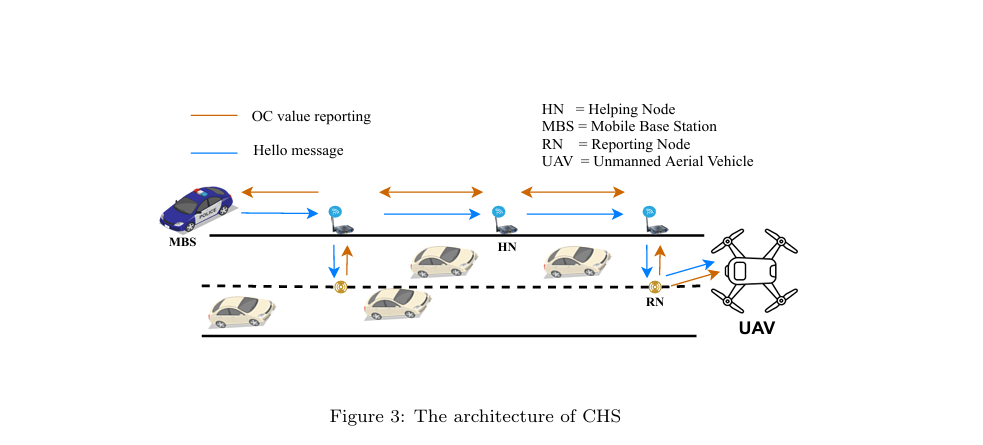
\includegraphics[width=0.7\textwidth]{Figures/Chapter3/Method6/1.png}
    \caption{CHS System Architecture (Source: \cite{bashir2022closed})}
    \label{fig:chs_architecture}
\end{figure}

\vspace{\baselineskip} % Add a line space between paragraphs

\subsection{Probabilistic Model for UAV Trajectory Control}
The CHS system employs a probabilistic approach to manage the UAV’s flight trajectory. Overspeeding incidents are modeled as a Poisson process, where the Overspeeding Count (OC) represents the average rate of violations over a given time period. The Poisson distribution function for a random variable \( Y \) is given by:

\begin{equation}
P(Y = y) = \frac{\lambda^y e^{-\lambda}}{y!}
\label{eq:poisson}
\end{equation}

where:
\begin{itemize}
    \item \( \lambda \) is the mean success rate (average OC value).
    \item \( e \) is Euler’s number.
    \item \( y \) is the actual number of overspeeding incidents in a defined time frame.
\end{itemize}

The UAV calculates the probability of detecting overspeeding incidents at each RN using the following steps:
\begin{enumerate}
    \item \textbf{Probability of Fewer Incidents:} The probability of an RN detecting fewer than \( OC_{max} \) overspeeding vehicles is calculated as:
    \begin{equation}
    Pr(Y < OC_{max}) = \sum_{y=0}^{OC_{max}-1} \frac{(OC_{rtn-1})^y e^{-OC_{rtn-1}}}{y!}
    \label{eq:prob_less}
    \end{equation}

    \item \textbf{Probability of More Incidents:} The probability of an RN detecting at least \( OC_{max} \) overspeeding vehicles is:
    \begin{equation}
    Pr(Y \geq OC_{max}) = 1 - Pr(Y < OC_{max})
    \label{eq:prob_more}
    \end{equation}

    \item \textbf{Travel Time Adjustment:} The UAV adjusts its trajectory based on the travel time between RNs, calculated as:
    \begin{equation}
    t_{r,x} = \frac{d_{r,x}}{v}
    \label{eq:travel_time}
    \end{equation}
    where \( d_{r,x} \) is the distance between RNs \( r \) and \( x \), and \( v \) is the UAV’s speed.
\end{enumerate}

The UAV uses these probabilities to determine its next position, prioritizing RNs with the highest likelihood of overspeeding incidents. Figure~\ref{fig:uav_movement} illustrates the UAV’s movement based on probabilistic calculations.

\begin{figure}[h]
    \centering
    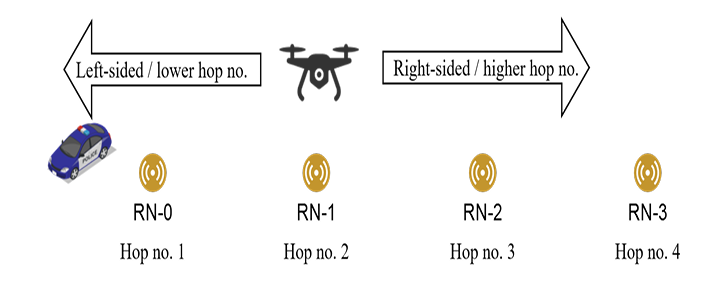
\includegraphics[width=0.7\textwidth]{Figures/Chapter3/Method6/2.png}
    \caption{Movement Control Algorithm and Hop Count Assignment (Source: \cite{bashir2022closed})}
    \label{fig:hop_numbers}
\end{figure}

\vspace{\baselineskip} % Add a line space between paragraphs

\subsection{Hop Number Allocation and Instant Reporting}
The Mobile Base Station (MBS) broadcasts hello messages to assign hop numbers to UAVs and wireless nodes. This process ensures efficient data routing and communication within the network. Key features include:
\begin{itemize}
    \item \textbf{Hop Number Assignment:} Each node updates its hop number based on the received hello message and rebroadcasts it with an incremented hop count.
    \item \textbf{Instant Reporting:} Severe speed violations are reported immediately to the MBS, while less critical violations are transmitted when the UAV is near the MBS.
\end{itemize}

Figure~\ref{fig:hop_numbers} illustrates the hop number assignment procedure.

\vspace{\baselineskip} % Add a line space between paragraphs

\subsection{Performance Evaluation}
The performance of the CHS system was evaluated through simulations using Network Simulator-2 (NS-2). Four traffic scenarios were tested to assess the system’s ability to minimize UAV movements while maximizing overspeeding detection. The results were compared with two existing methods:
\begin{itemize}
    \item \textbf{Static:} The UAV remains stationary at a fixed hotspot.
    \item \textbf{Stepwise:} The UAV follows a predefined trajectory without adapting to real-time data.
\end{itemize}

\subsubsection{Key Metrics}
The evaluation focused on three metrics:
\begin{enumerate}
    \item \textbf{Detection Rate:} The number of overspeeding incidents detected by the UAV.
    \item \textbf{Response Time:} The delay in reporting critical violations to the MBS.
    \item \textbf{Energy Efficiency:} The UAV’s energy consumption during surveillance.
\end{enumerate}

\subsubsection{Simulation Results}
\begin{itemize}
    \item \textbf{Simulation-I:} When RN-2.0 was the dominant hotspot, the Static-2.0 scheme detected the most violations. However, the CHS system performed similarly by dynamically adjusting to the hotspot.
    \item \textbf{Simulation-II:} When RN-3.9 became the dominant hotspot, Static-3.9 outperformed other static schemes, while CHS adapted effectively by relocating the UAV to RN-3.9.
    \item \textbf{Simulation-III:} With RN-5.3 as the dominant hotspot, Static-5.3 detected the most violations, while CHS maintained high detection rates by balancing movement and monitoring.
    \item \textbf{Simulation-IV:} In a dynamic scenario with shifting hotspots, CHS outperformed all static and stepwise schemes by continuously adapting to real-time data.
\end{itemize}

\begin{table}[h]
    \centering
    \caption{Simulation Parameters}
    \label{tab:simulation_params}
    \begin{tabular}{|l|c|}
        \hline
        \textbf{Parameter} & \textbf{Value} \\
        \hline
        Network size & 10 m \(\times\) 10000 m \\
        UAV speed & 15 m/s \\
        Transmission range & 100 m \\
        Number of wireless nodes & 78 \\
        Number of vehicles & 200–300 \\
        Vehicle speed range & 13–27 m/s \\
        OC reporting interval & 100 s \\
        Simulation time & 0–2500 s \\
        \hline
    \end{tabular}
\end{table}

\vspace{\baselineskip} % Add a line space between paragraphs

\subsection{Limitations and Challenges}
While the CHS system demonstrates significant potential, it faces several limitations:
\begin{itemize}
    \item \textbf{Energy Constraints:} UAVs have limited battery life, which restricts their operational duration. Frequent recharging or battery replacement is required, especially in large-scale deployments.
    \item \textbf{Communication Reliability:} The system relies on IEEE 802.11p for communication, which is susceptible to interference and signal degradation in urban environments.
    \item \textbf{Environmental Sensitivity:} Adverse weather conditions, such as heavy rain or strong winds, can affect UAV stability and communication.
    \item \textbf{Real-Time Processing:} The system assumes real-time processing of traffic data, but delays in data transmission or processing could impact its responsiveness.
    \item \textbf{Regulatory Restrictions:} UAV operations are subject to strict regulations, including altitude limits and no-fly zones, which could hinder widespread adoption.
\end{itemize}

\vspace{\baselineskip} % Add a line space between paragraphs


%%%%%%%%%%%%%%%%%%%%%%%%%%%%% Conclusion %%%%%%%%%%%%%%%%%%%%%%%%%%%%%


\section{Conclusion}

The six methods discussed in this chapter illustrate the diverse and innovative approaches to UAV-based traffic monitoring, each addressing specific challenges in traffic surveillance and management. From early systems like the Airborne Traffic Surveillance System (ATSS) to advanced frameworks such as Collaborative Hotspot Selection (CHS), these methods demonstrate the potential of UAVs to revolutionize traffic monitoring by providing real-time, adaptive, and scalable solutions. Key advancements include the integration of 5G technology for high-speed communication, probabilistic models for dynamic UAV trajectory control, and cooperative systems that leverage multiple UAVs for comprehensive coverage.

\vspace{\baselineskip} % Add a line space between paragraphs

Despite their promise, these methods face several challenges that must be addressed for practical deployment. Energy constraints, communication reliability, and regulatory restrictions remain significant barriers to the widespread adoption of UAV-based traffic monitoring systems. Additionally, environmental factors such as adverse weather conditions and line-of-sight limitations can impact system performance. However, ongoing advancements in UAV technology, artificial intelligence, and wireless communication networks offer promising avenues for overcoming these challenges.

\vspace{\baselineskip} % Add a line space between paragraphs

In conclusion, UAV-based traffic monitoring systems represent a significant leap forward in traffic management, offering unparalleled flexibility, efficiency, and adaptability. By addressing the limitations of traditional systems and leveraging the unique capabilities of UAVs, these methods pave the way for smarter, safer, and more efficient urban transportation networks. As research and development in this field continue, the integration of UAVs into traffic monitoring systems is expected to play a pivotal role in shaping the future of intelligent transportation systems.

\chapter*{Syntheses}

The rapid evolution of UAV technology presents unprecedented opportunities for transforming traffic surveillance and management systems. Across the three chapters, we observe how foundational advancements in UAV architectures and communication protocols enable increasingly sophisticated applications. The development of specialized communication standards and decentralized network architectures has addressed critical challenges in reliability and scalability for UAV operations. These technical foundations support the integration of AI-driven optimization techniques that enhance autonomous decision-making while maintaining robust security against emerging cyber threats.

\vspace{0.5cm}

Practical implementations demonstrate the versatility of UAV systems in traffic monitoring applications, from basic surveillance to complex cooperative frameworks. The successful deployment of 5G-enabled systems and probabilistic control models shows particular promise for real-time traffic management. However, these technological achievements must be balanced against persistent limitations in operational endurance, communication stability, and regulatory frameworks. Addressing these constraints through continued innovation in energy systems, network protocols, and policy development will determine the pace of UAV adoption in transportation infrastructure.

\vspace{0.5cm}

Looking ahead, the convergence of these technical domains - communication systems, artificial intelligence, and practical applications - points toward a future where UAV networks become integral components of smart city ecosystems. The research presented in these chapters establishes both the current state of the art and critical pathways for future development in this dynamic field. As these technologies mature, they will enable more responsive, efficient, and intelligent transportation networks capable of meeting the growing demands of urban mobility.

% Print the bibliography
\printbibliography[heading=bibintoc, title=References]  % This adds to TOC automatically

\end{document}